\documentclass[12pt]{report}
\usepackage{suthesis}
%\documentstyle[12pt,suthesis]{report}

% -- Imports --
% (general libraries)
\usepackage{times,latexsym,amsfonts,amssymb,amsmath,graphicx,bbm,rotating}
\usepackage{enumitem,multirow,hhline,stmaryrd,bussproofs,mathtools,siunitx,arydshln}
\usepackage{booktabs,xcolor,csquotes}
% (custom libraries)
\usepackage{fitch}
% (inline references)
\usepackage[square,sort,comma,numbers]{natbib}
% (tikz)
\usepackage{tikz}
\usetikzlibrary{shapes.arrows,chains,positioning,automata,trees,calc}
\usetikzlibrary{patterns}
\usetikzlibrary{decorations.pathmorphing,decorations.markings}
% (tikz dependency tree)
\usepackage{tikz-dependency,pifont}
% (print algorithms)
\usepackage[ruled,lined,linesnumbered]{algorithm2e}
% (custom)
\input std-macros.tex
\input macros.tex	
% (paper compilation hacks)
\def\newcite#1{\citet{#1}}
\definecolor{darkblue}{rgb}{0.0,0.0,0.4}

%% Thang
\usepackage{epigraph}
\renewcommand{\epigraphsize}{\small}
\setlength{\epigraphwidth}{0.8\textwidth}
\usepackage{pstricks} % for overlay latex on top of images

% to split on hyphens for long urls
\usepackage{url}
\makeatletter
\g@addto@macro{\UrlBreaks}{\UrlOrds}
\makeatother
% the below works for pdflatex
%\usepackage[hyphens]{url} 
\usepackage{hyperref}


\definecolor{lightgreen}{HTML}{44B178}
\definecolor{lightblue}{HTML}{3B8CDA}
\newcommand{\error}[1]{{\color{red} #1}}
\newcommand{\ngram}{$n$-gram}
\newcommand{\word}[1]{``#1''}
\newcommand{\bfit}[1]{\textbf{\textit{#1}}}
\newcommand{\unk}{$<$\texttt{unk}$>$}
\newcommand{\sos}{$<$\texttt{sos}$>$}
\newcommand{\eos}{$<$\texttt{eos}$>$}
\newcommand{\eq}[1]{Eq.~(\ref{#1})}
\newcommand{\lemmaref}[1]{Lemma~\ref{#1}}
\newcommand{\figref}[1]{Figure~\ref{#1}}
\newcommand{\nlmtext}{neural probabilistic language models}
\newcommand{\nlm}{NPLM}
\newcommand{\nlms}{NPLMs}
\newcommand{\secref}[1]{Section~(\ref{#1})}
\newcommand{\algo}[1]{Algorithm~\ref{#1}}

% math operators
%\DeclareMathOperator*{\argmax}{\arg\,\max}
%\DeclareMathOperator{\diag}{diag}
\DeclareMathOperator{\e}{e}
\DeclareMathOperator{\trace}{Tr}
\DeclareMathOperator{\sigm}{sigm}
\DeclareMathOperator{\sigmoid}{sigmoid}
\DeclareMathOperator{\softmax}{softmax}
\DeclareMathOperator{\Index}{Index}

% math
\newcommand{\MB}[1]{\mbox{\boldmath{$#1$}}} % boldface for matrix and vectors
% derivative fractions
\newcommand{\parfrac}[1]{\frac{\partial}{\partial #1}} 
% fraction derivatives
\newcommand{\fracder}[2]{\frac{\partial #1}{\partial #2}}
% sum and product
\newcommand{\sumkn}{\sum_{k=1}^{n}} %I use this when deriving backprop eqns. n is the LSTM block size and k is a better choice than i because it won't get confused with the input gate
% plus equal
\newcommand{\pluseq}{\mathrel{+}=}
% transpose
\newcommand{\tp}[1]{#1^\top}
% round bracket
\newcommand{\open}[1]{\left(#1\right)}
\newcommand{\paren}[1]{\left(#1\right)}
% norm
\newcommand{\norm}[1]{\left\lVert#1\right\rVert}
% grad
\newcommand{\grad}[1]{\nabla #1}

%%% math commands %%%
% variables 
\usepackage{bm}
\newcommand{\x}[1]{\bm{x}_{#1}}
\newcommand{\y}[1]{\bm{y}_{#1}}
\newcommand{\z}[1]{\bm{z}_{#1}}
\newcommand{\s}[1]{\bm{s}_{#1}}
\newcommand{\prob}[1]{\bm{p}_{#1}}
\newcommand{\der}[1]{d\bm{#1}}
\newcommand{\W}[1]{\bm{W}_{#1}}
\newcommand{\inR}[1]{\in \mathbb{R}^{#1}}
\newcommand{\yrange}[2]{y_{\overline{#1,#2}}}
\newcommand{\ytop}[1]{y^{(#1)}}
\newcommand{\thetav}{\bm{\theta}}

\newcommand{\edot}{\circ}
% lstm
\newcommand{\mem}[1]{\bm{c}_{#1}}
\newcommand{\ig}{\bm{i}_{t}}
\newcommand{\fg}{\bm{f}_{t}}
\newcommand{\og}{\bm{o}_{t}}
\newcommand{\hg}{\MB{\hat{h}_t}}
%\newcommand{\iparam}{\MB{T}_{\text{i}}} % input params 
%\newcommand{\fparam}{\MB{T}_{\text{f}}} % forget params 
%\newcommand{\oparam}{\MB{T}_{\text{o}}} % output params 
\newcommand{\hparam}{\MB{T}_{\text{h}}} % hidden params 
\newcommand{\xparam}{\MB{T}_{\text{x}}} % hidden params 
\newcommand{\ut}{\bm{u}_t}

% NMT
\newcommand{\tgt}[1]{y_{#1}} % target word
\newcommand{\src}[1]{x_{#1}} % source word
\newcommand{\al}{\MB{a}_{t}} % align
\newcommand{\hid}[1]{\bm{h}_{#1}}
\newcommand{\his}{\MB{\bar{h}}_{s}} % hidden top source
\newcommand{\hs}{\MB{\tilde{h}}_{t}} %h softmax
\newcommand{\hd}[1]{\MB{h}_{#1}} % hidden target 
\newcommand{\hb}[1]{\MB{\bar{h}}_{#1}} % hidden source
%\newcommand{\rnn}{\MB{T}_{d \times 2d}} % RNN
\newcommand{\rnn}{\MB{T}_{\text{rnn}}} % RNN
% \newcommand{\lstm}{\MB{T}_{4d \times 2d}} % lstm 
\newcommand{\lstm}{\MB{T}_{\text{lstm}}} % LSTM 
\newcommand{\hi}{\MB{h}_{t}} % hidden top
\newcommand{\co}{\MB{c}_{t}} % context


%% Abi
\usepackage{amsthm} %for the proof environment
%theorem environments
\newtheorem{theorem}{Theorem}
\newtheorem{lemma}{Lemma}
\newtheorem{definition}{Definition}
\newtheorem{claim}{Claim}
\newtheorem{corollary}{Corollary}

%% Chapter 3
\newcommand{\unkword}[1]{{\bf {\it {\underline{#1}}}}}
\newcommand{\unksym}{{\it \texttt{\underline{unk}}}}
\newcommand{\eossym}{$<$\texttt{eos}$>$}
\newcommand{\unkcopy}[1]{{\bf {\it {\texttt{\underline{unk}$_{#1}$ }}}}}
\newcommand{\unknull}{{\bf {\it {\texttt{\underline{unk}$_{\emptyset}$}}}}}
\newcommand{\unktext}[1]{{\bf {\it \texttt{\underline{unk}}$_{#1}$}}}
\newcommand{\pos}[1]{{\bf {\it {\texttt{p$_{#1}$}}}}}
\newcommand{\posnull}{{\bf {\it {\texttt{p$_{\emptyset}$}}}}}
\newcommand{\postext}[1]{{\bf {\it \texttt{p}$_{#1}$}}}
\newcommand{\unkpos}[1]{{\bf {\it {\texttt{\underline{unkpos}$_{#1}$}}}}}
\newcommand{\unkpostext}[1]{{\bf {\it \texttt{unkpos}$_{#1}$}}}

% experiment results
\newcommand{\bestbleu}{35.6}
\newcommand{\bestbleuunk}{37.5} % after unk translation
\newcommand{\bestbleuunkwmt}{36.6} % after unk translation
\newcommand{\bestunkimp}{2.8} % best of (bleuunk - bleu)
\newcommand{\unkimp}{1.9} % bestbleuunk - bestbleu
\newcommand{\unkimpilya}{2.7} % compare with ilya best system 34.8
\newcommand{\imprare}{4.8} % compare the last group of 500 sentences with the most rare words before and after unk translations (in Rarity Analysis)

%% Chapter 4
\newcommand{\correct}[1]{\textit{\color{blue} #1}}
\newcommand{\wrong}[1]{\textbf{\color{red} #1}}
\newcommand{\pt}{p_{t}} % context
\newcommand{\sotaold}{23.0} % WMT'14 English-German
\newcommand{\sotanew}{25.9} % WMT'15 English-German
\newcommand{\attngain}{5.0} % max improvement when using attention 
\newcommand{\localm}{local-m} % max improvement when using attention 
\newcommand{\localp}{local-p} % max improvement when using attention 
\DeclareMathOperator{\alignf}{align}
\DeclareMathOperator{\score}{score}

%% Chapter 5
\newcommand{\hide}[1]{}
\newcommand{\source}[1]{\bi{#1}}
\newcommand{\close}[1]{\underline{\color{brown} #1}}
% char
\newcommand{\Ww}{\MB{W}} % W_h 
\newcommand{\Wc}{\MB{\breve{W}}} % W_c
\newcommand{\hc}{\MB{\breve{h}}_{t}} %h softmax char

\newcommand{\hybrid}{hybrid-NMT}
\newcommand{\rare}{$<${\it rare}$>$}

% best models
\newcommand{\modelword}{{\it (d)}}
\newcommand{\modelchar}{{\it (g)}}
\newcommand{\modelsmall}{{\it (k)}}
\newcommand{\model}{{\it (l)}}
\newcommand{\ensbleu}{20.7}
\newcommand{\gain}{2.1{-}11.4}
\newcommand{\chr}{chrF$_3$}




% -- Document --
\begin{document}

% Title
\title{Neural Machine Translation}
\author{Minh-Thang Luong}
\principaladviser{Christopher D. Manning}
\firstreader{Dan Jurafsky}
\secondreader{Andrew Ng}
\thirdreader{Quoc V. Le}

% Preface
\beforepreface
%\input preface.tex
%\input ack.tex
\afterpreface


% -- Sections --
\chapter{Introduction}
\label{c:intro}
\epigraph{The Babel fish is small, yellow, leech-like, and probably the oddest
thing in the universe. It feeds on brainwave energy  ...
%absorbing all unconscious
%frequencies and then excreting telepathically a matrix formed from the conscious
%frequencies and nerve signals picked up from the speech centres of the brain,
%the practical upshot of which is that 
if you stick a Babel fish in your ear, you can
instantly understand anything in any form of language.}{{\it The Hitchhiker's
Guide to the Galaxy}. Douglas Adams.}
Human languages are diverse %and rich in categories 
with about 6000 to 7000
languages spoken worldwide \cite{languages}.
As civilization advances, the need for seamless communication and understanding across
languages becomes more and more crucial. Machine translation (MT), the
task of teaching machines to learn to translate automatically across languages, as
a result, is an important research area.
MT has a long history \cite{hutchins07} from the original
phiosophical ideas of universal languages in the $17^{\text{th}}$ century to
%first practical instances of MT in the twentieth century, e.g., one proposal by \newcite{weaver49}. 
\edit{
those first practical suggestions in the 1950s, most notably an influential %important
proposal by \newcite{weaver49} which marked the beginnings of MT research in
the United States. In that memorandum, Warren Weaver touched on
the idea of using computers to translate, specifically addressing the language
ambiguity problem by combining his knowledge of statistics,
cryptography, information theory, as well as logical and linguistic universals
\cite{hutchins2000early}.
Since then, MT has gone through many
periods of great development but also encountered several stagnant phases as
illustrated in \figref{f:mt_progress}.
Despite several moments of excitement that led to hopes that MT
will be solved ``very soon'' such as the 701 translator \cite{ibm701}
developed by scientists at Georgetown and IBM in the 1950s and the popular Google Translate
%or a simple vector-space transformation
%technique \cite{vectorspace} proposed by Google researchers 
at the beginning of the $21^{\text{st}}$ century \cite{brants07},
MT remains an extremely challenging problem \cite{solvemt,winograd_mt16}.
This motivates my work in the area of machine translation; specifically,
in this thesis, the goal is to advance neural machine translation (NMT), a new
promising approach for MT developed just recently, over the past two years. The results achieved in this
thesis on NMT together with work from other researchers have eventually
 produced a significant leap in the translation quality as illustrated in
\figref{f:mt_progress}. Before delving into details of the thesis, we now walk
the audience through the background and a bit of the development history of
machine translation.
}
%To understand why MT is difficult, let us trace through one ``evolution''
%path of % development
%MT which crosses through techniques that are used extensively in
%commercial MT systems. 

\begin{figure}[tbh!]
\centering
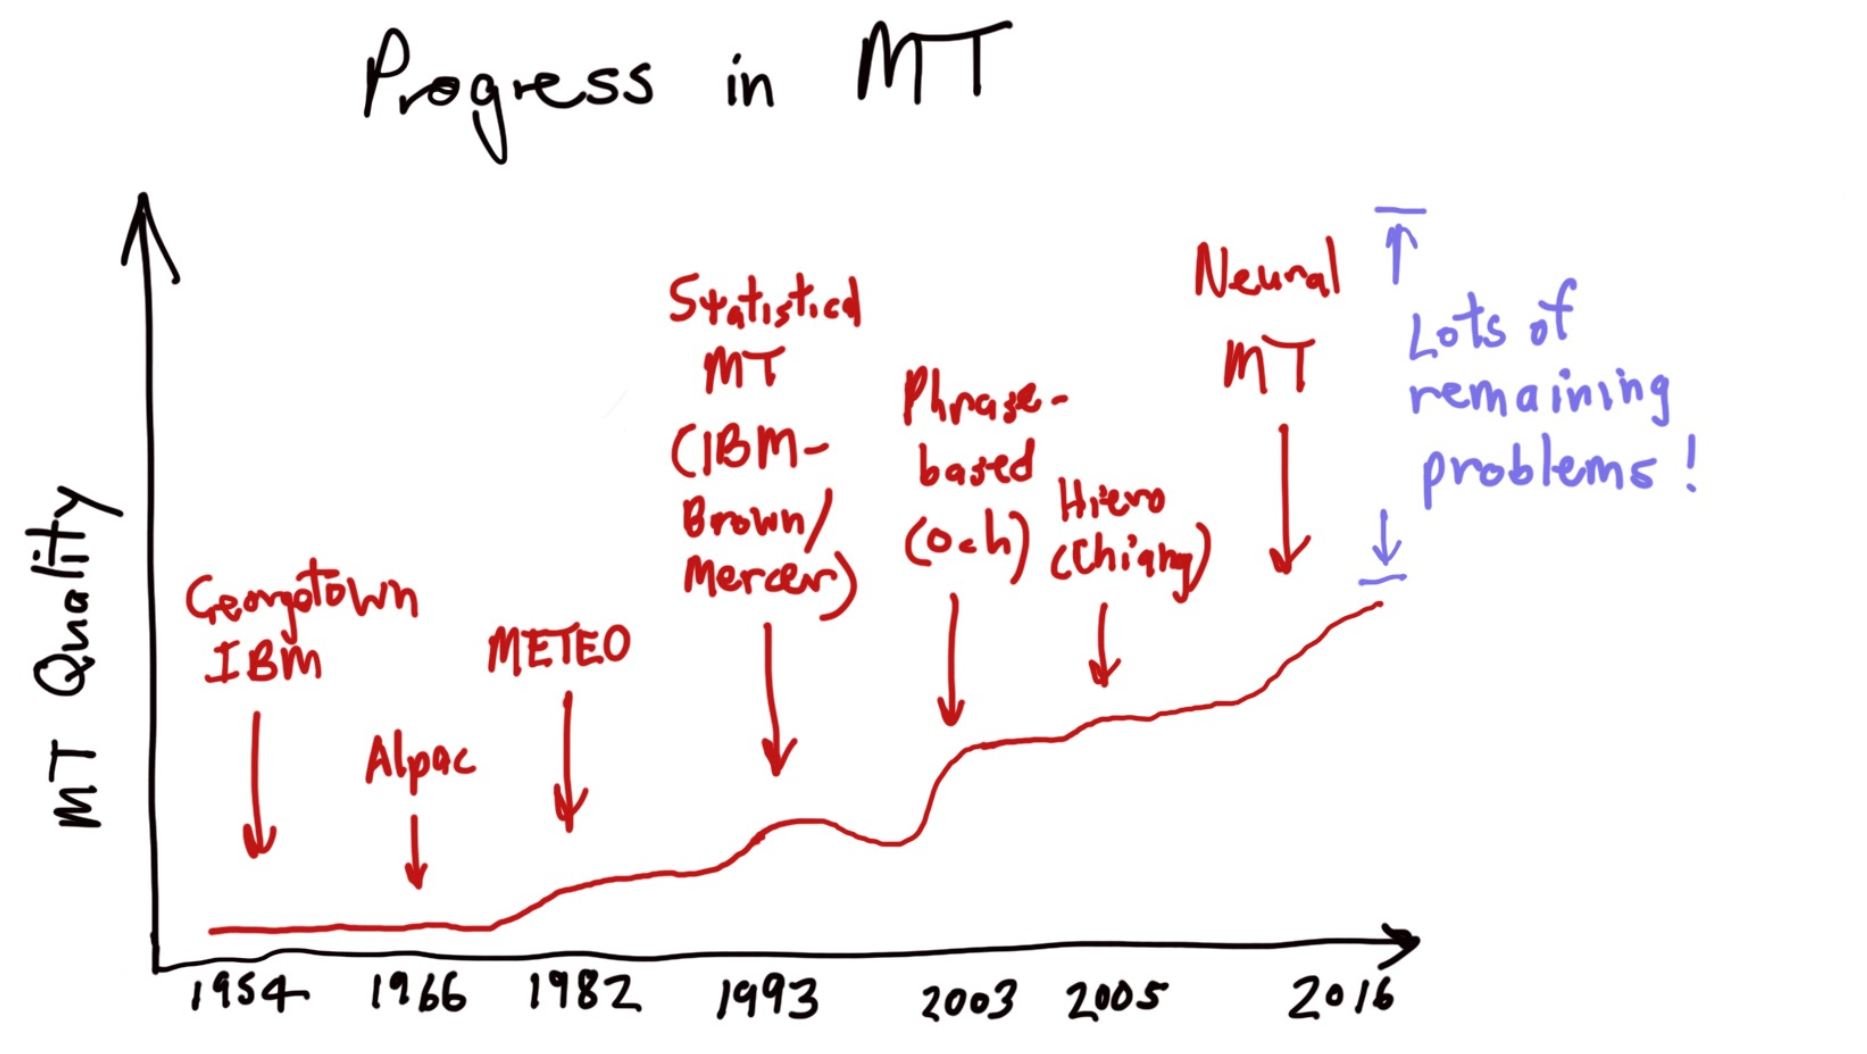
\includegraphics[width=\textwidth, clip=true, trim= 0 0 20 80]{img/MT_progress}
\caption[Machine translation progress]{{\bf Machine translation progress} --
from the 1950s, the starting of modern MT research, until the time of this
thesis, 2016, in which neural MT becomes a dominant approach. Image courtesy of
Christopher D. Manning.
} 
\label{f:mt_progress}
\end{figure}


\section{Machine Translation}
\begin{figure}
\centering
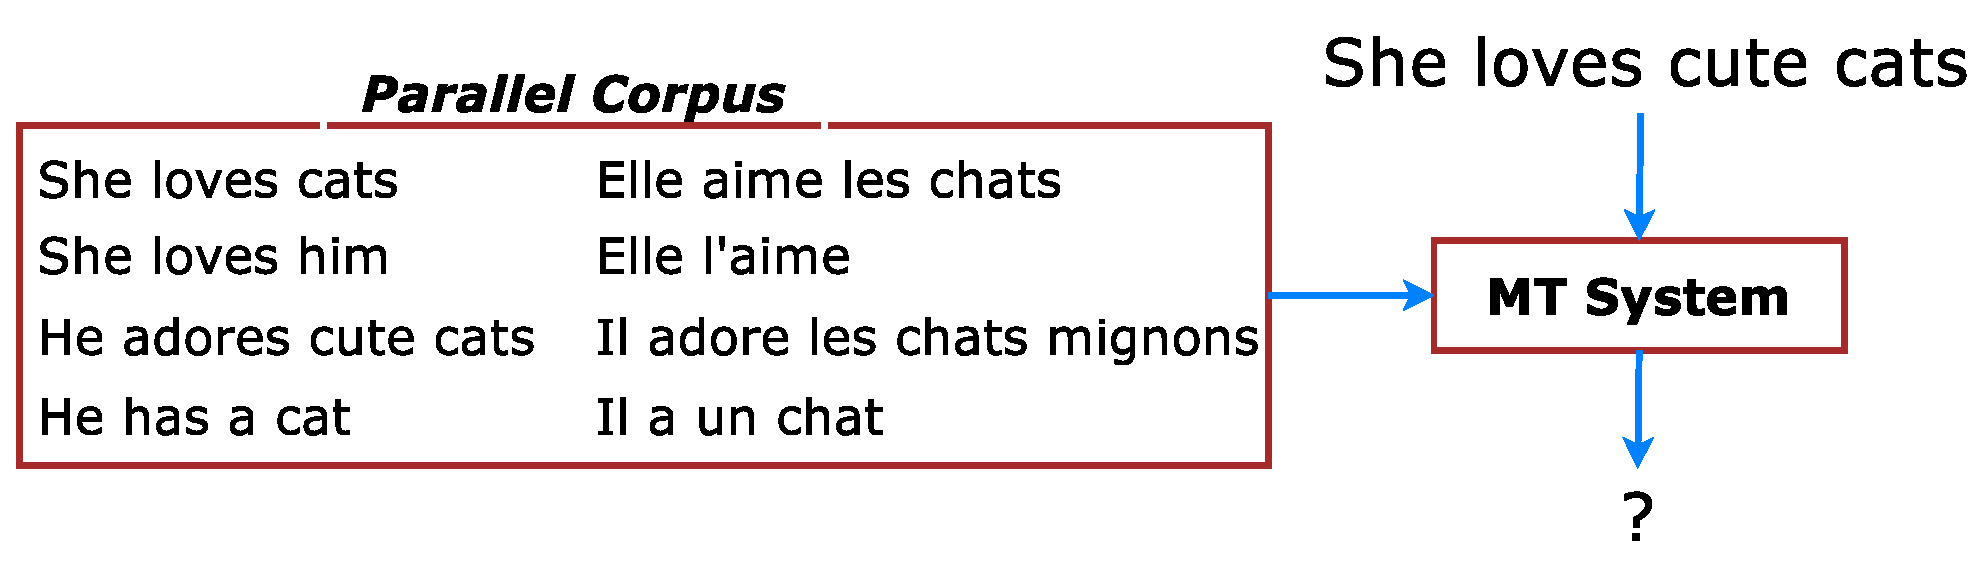
\includegraphics[width=\textwidth, clip=true, trim= 0 0 0 0]{img/mt.eps} % , angle=-90
\caption[Corpus-based approaches to machine translation]{{\bf Corpus-based approaches to
machine translation} -- a general setup in which MT systems
are built from parallel corpora of sentence pairs having the same meaning. Once
built, systems are used to translate new unseen
sentences, e.g., \word{She loves cute cats}.}
\label{f:mt}
\end{figure}

\edit{
Despite much enthusiasm, the beginning period of MT research in the 1950-60s,
was mostly about direct word-for-word replacement based on bilingual
dictionaries.\footnote{There are also proposals for ``interlingual'' and
``transfer'' approaches but these seemed to be too challenging to achieve, not
to mention limitations in hardware at that time\cite{hutchins07}.} An MT winner quickly came
right after the ALPAC report in 1966 pointing out that ``there is no immediate
or predictable prospect of useful machine translation'', which hampered MT
research for over a
decade. Fast-forwarding through the resurgence in the 1980s beginning with
Europe, Japan, and gradually the United States,
}
modern statistical MT started out with a seminal work by IBM scientists
\cite{Brown:1993:MSM}. The proposed {\it corpus-based} approaches require
minimal linguistic content and only need a {\it parallel} dataset of
sentence pairs which are translations of one
another, to train MT systems.
Such a language-independent setup is illustrated in Figure~\ref{f:mt}. 
\edit{
In more
detail, instead of hand building bilingual dictionaries which can be costly to
obtain, Brown and colleagues proposed to learn these dictionaries, or {\it
translation models}, probabilistically from parallel corpora. To accomplish
this, they propose a series of 5 algorithms of increasing complexity, often
referred as IBM Models 1-5, to learn {\it word alignment},
a mapping between source and target words in a parallel corpus, as illustrated
in \figref{f:wordalign}. The idea is
simple: the more often two words, e.g., \word{loves} and \word{aime}, occur
together in different sentence pairs, the more likely they are aligned to each
other and have equivalent meanings.
}

\begin{figure}[tbh!]
\centering
\includegraphics[width=0.35\textwidth, clip=true, trim= 0 0 0
0]{img/wordalign.eps}
\caption[Word-based alignment]{{\bf Word-based alignment} -- example of
an alignment between source and target words. In IBM
alignment models, each target word is aligned to at most one source word.
} 
\label{f:wordalign}
\end{figure}

\edit{
Once a translation model, i.e., a probabilistic bilingual dictionary, has been
learned, IBM model 1, the simplest and the most na\"{i}ve one among the five proposed
algorithms, translates a new source sentence as follows. First, it decides on
how long the translation is as well as how source words will be mapped to target
words as illustrated in Step 1 of \figref{f:wordmt_algo}. Then,
in Step 2, it produces a translation by selecting for each target position a
word that is the best translation for the aligned source word according to the
bilingual dictionary. Subsequent IBM models build on top of one another and refine the
translation story such as better modeling the reordering structure, i.e., how
word positions differ between source and target languages. We refer the audience to
the original IBM paper or Chapter 25 of \cite{Jurafsky:2009} for more details.
}
\begin{figure}[tbh!]
\centering
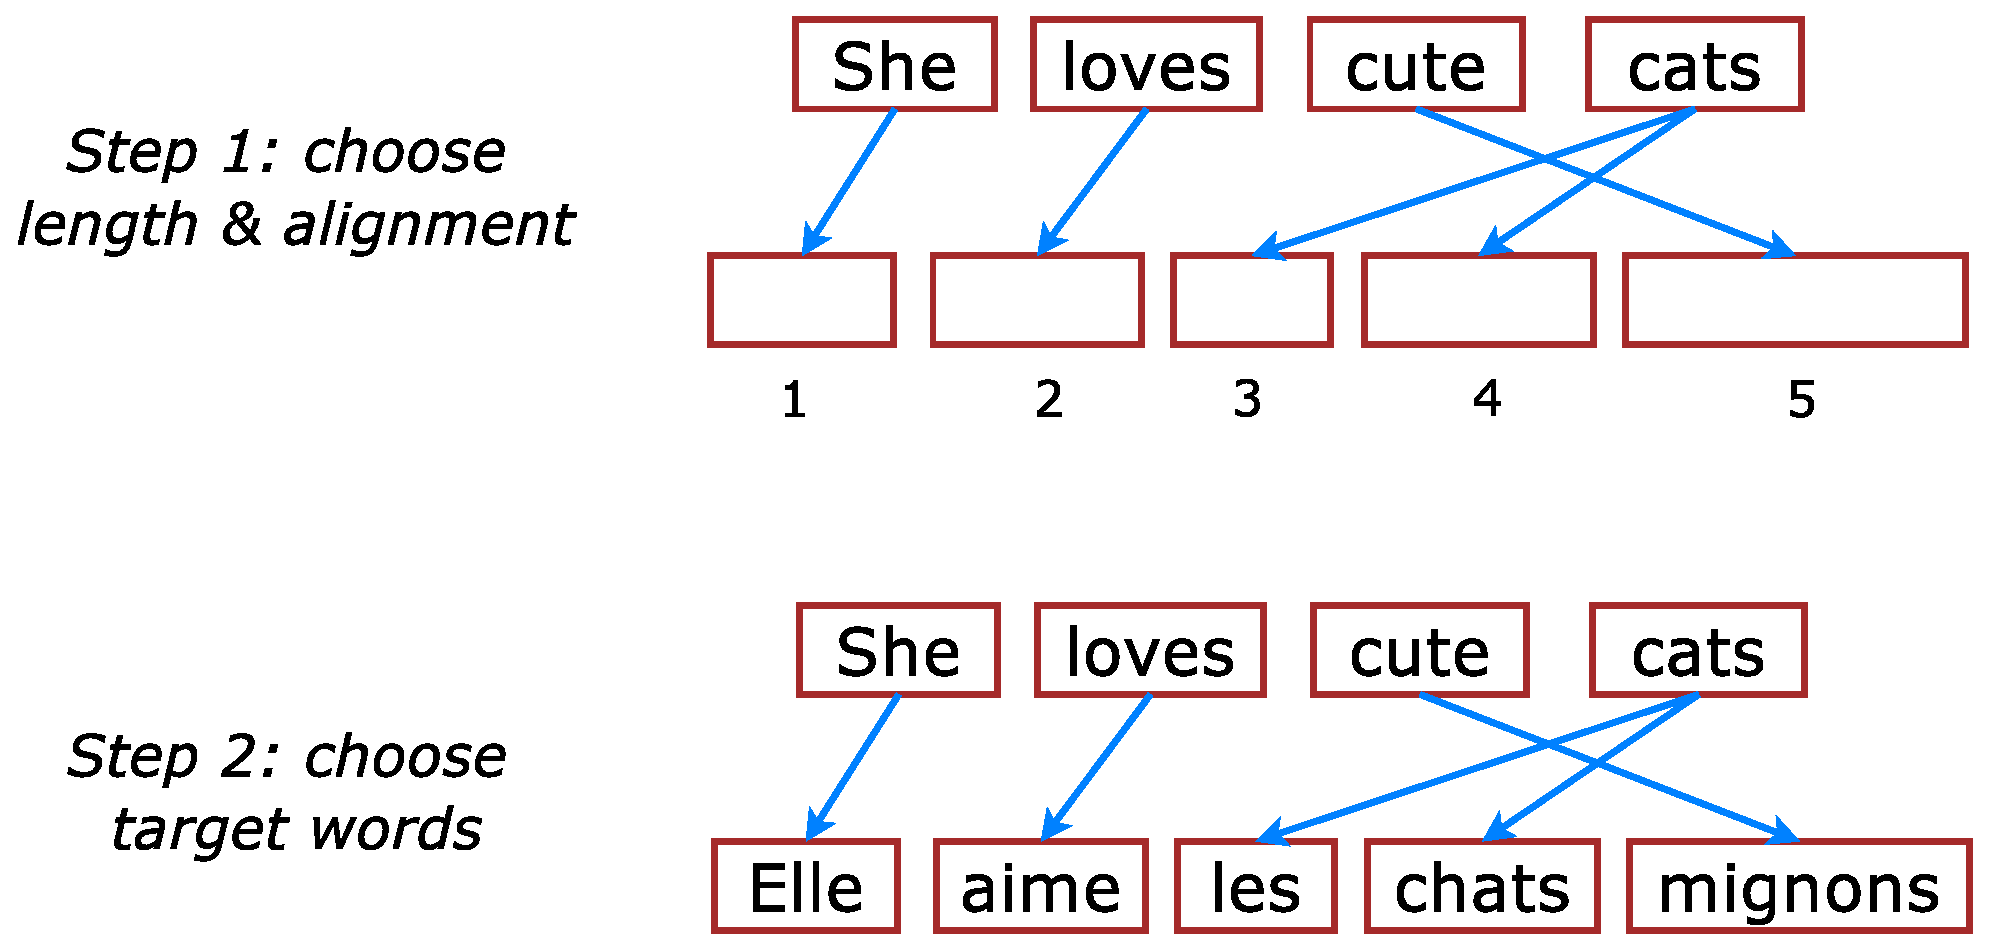
\includegraphics[width=0.8\textwidth, clip=true, trim= 0 0 0
0]{img/wordmt_algo.eps} % , angle=-90
\caption[A simple translation story]{{\bf A simple translation story} -- example of the generative story in
IBM Model 1 to produce a target translation given a source sentence and a
learned translation model.
} 
\label{f:wordmt_algo}
\end{figure}

\edit{
There are, however, two important details that we left out in the above translation story,
the {\it search} process and the {\it language modeling} component. In Step 1,
one might wonder among the exponentially many choices, how do we know what the
right translation length is and how source words should be mapped to target words? The
search procedure informally helps us ``browse'' through a manageable set of
candidates which are likely to include a good translation; whereas, the language
model will help us select the best translation among these candidates. We will
defer details of the search process to later since it is dependable on the
exact translation model being used. Language modeling, on the other hand, is an
important concept which has been studied earlier in speech recognition
\cite{katz87}. In a nutshell, a language model (LM)
learns from a corpus of monolingual text in the target language and collect
statistics on which sequence of words are likely to go with one another. When
applying to machine translation, an LM will assign high scores for coherent and
natural-sounding translations and low scores for bad ones.
For our example in the above figure, if the model happens to choose a wrong alignment, e.g.,
\word{cute} goes to position 3 while \word{cats} goes to positions 4 and 5, an
LM will alert us with a lower score given to that incorrect translation \word{Elle
aime mignons les chats} compared to the translation \word{Elle aime les chats
mignons} with a correct word ordering structure.\footnote{
\edit{
For completeness, translation and
language models are integrated together in an MT system through the {\it
Bayesian noisy channel} framework as follows:
\begin{align}
\label{e:noisy}
\hat{t} &= \argmax_t P(t|s) \approx \argmax_t P(s|t) P(t)
\end{align}
Here, we have a source sentence $s$ in which we ask our {\it decoder}, an
algorithm that implements the aforementioned search process, to find the best
translation, the $\argmax$ part. $P(s|t)$ represents the {\it translation} model, the
faithfulness of the translation in terms of meaning preservation between the source and the
target sentences; whereas $P(t)$
represents the {\it language} model, the fluency of the translated text.
}
}

While the IBM work had a huge impact on the field of statistical MT, researchers
quickly realized that word-based MT is insufficient as words
require context to properly translate, e.g., \word{bank} has two totally different
meanings when preceded by \word{financial} and \word{river}. As a result,
{\it phrase-based models}, \cite{Marcu:2002,Zens2002,Koehn:2003:SMT}, inter alia, became the de facto
standard in MT research and are still being the dominant approach in existing
commercial systems such as Google Translate until now. Much credit went to Och's
work on {\it alignment templates}, starting with his thesis in 1998 and later in
\cite{och03,och04}. The idea of alignment templates is to enable phrase-based MT
by first symmetrizing\footnote{\edit{Symmetrization is achieved by training IBM models
in both directions, source to target and vice versa, then intersecting the
alignments. There are subsequent techniques that jointly train alignments in
both directions such as \cite{liang06alignment}.}} the alignment to obtain many-to-many correspondences
between source and target words; in contrast, the original IBM models only produce
one-to-many alignments. From the symmetrized alignment, several heuristics have
been proposed to extract phrase pairs; the general idea is that phrase
pairs need to be ``consistent'' with their alignments: each word in a phrase
should not be aligned to a word outside of the other phrase. These pairs are stored
in what called a {\it phrase table} together with various scores to evaluate
phrase pairs in different aspects, e.g., how equivalent the meaning is, how good
the alignment is, etc. \figref{f:phrase_mt} gives an example of how a
phrase-based system translates.
}

\begin{figure}[tbh!]
\centering
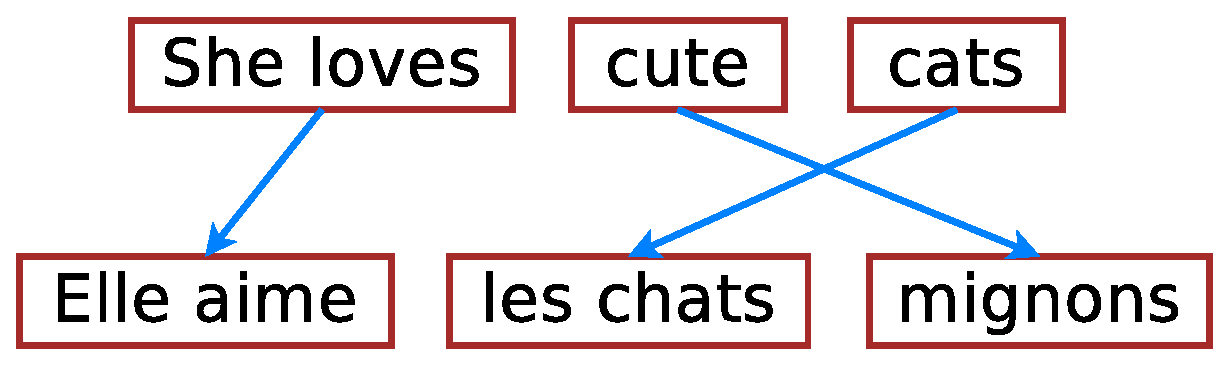
\includegraphics[width=0.45\textwidth, clip=true, trim= 0 0 0
0]{img/phrasemt.eps} % , angle=-90
\caption[Phrase-based machine translation]{{\bf Phrase-based machine translation} (MT) -- example of how phrase-based
MT systems translate a source sentence \word{She loves cute cats} into a target sentence
\word{Elle aime les chats mignons}: sentences are split into chunks and phrases
are translated.
} 
\label{f:phrase_mt}
\end{figure}

%% log-linear models %%
\edit{
State-of-the-art MT systems, in fact, contain more components than just the two
basic translation and language models. There are many knowledge
sources that can be useful to the translation task, e.g., language model,
translation model, reversed translation model, reordering model, word penalty,
phrase penalty, unknown-word penalty, etc. To incorporate all of
these features, modern MT systems use a popular approach in natural language
processing, called the {\it maximum-entropy} or
{\it log-linear} models \cite{berger96,och02}, which has as its special case the
Bayesian noisy channel model that we briefly mentioned through \eq{e:noisy}.
Training log-linear MT models can be done using the standard {\it maximum
likelihood estimation} approach. However, in practice, these models are learned
by directly optimizing translation quality metrics such as BLEU
\cite{Papineni02bleu} in a technique known as {\it minimum error rate training}
or {\it MERT} \cite{och03mert}. Here, BLEU is an inexpensive automatic way of
evaluating the translation quality; the idea is to count words and phrases that
overlap between machine and human outputs.
}


%remains to be the general approach for nowadays MT systems.
%For over twenty years since the IBM seminal paper, approaches in MT
%such as
%\cite{Koehn:2003:SMT,och03,Liang:2006:EDA,koehn2007moses,chiang07hiero,dyer10cdec,cer10phrasal},
%%inter alia, 
%are, by and large, similar according to the following two-stage
%process (see Figure~\ref{f:phrase_mt}). First, source sentences are broken into
%chunks which can be translated in isolation by looking up a ``dictionary'', or
%more formally a {\it translation model}. Translated target words and phrases
%are then put together to form coherent and natural-sounding sentences by consulting a
%{\it language model} (LM) on which sequences of words, i.e., {\it \ngram{}s}, are
%likely to go with one another.

\section{Neural Machine Translation}
%% interlingual idea, Vaquois diagram %%
%% briefly mention syntax-based %%

The aforementioned approach, while has been successfully deployed in many commercial systems,
does not work very well and suffers from the following two major drawbacks.
First, translation decisions are {\it locally determined} as we translate
phrase-by-phrase and long-distance dependencies are often ignored. Second, it is
slightly ``strange'' that language models (LMs), despite being a key component in the MT
pipeline, utilize context information that is both short, consisting of only
a handful of previous words, and target-only, never looking at the source
words. These shortcomings in LMs gives rise to a new wave of {\it hybrid} systems which
aim to empower phrase-based MT with neural network components, most notably
\nlmtext{} (\nlms{}). 

\nlms{} were first proposed by \newcite{Bengio2003}
as a way to combat the ``curse'' of dimensionality suffered by traditional LMs.
In traditional LMs, one has to explicitly store and handle 
all possible \ngram{}s occurred in a training corpus, the number of which
quickly becomes enormous. As a result, existing MT systems often limit
themselves to use only short, e.g., $5$-gram, LMs \cite{kenlm}, which capture little context
and cannot generalize well to unseen \ngram{}s. \nlms{} address these concerns by
using distributed representations of words and not having to explicitly store
all enumerations of words. As a result, many MT systems, \cite{schwenk07,vaswani13decode,luong15nlm}, inter
alia, start adopting \nlms{} alongside with traditional LMs.
To make \nlms{} even more powerful, recent work
\cite{Schwenk12continuous,Son:2012:CST,Auli13,devlin14}
propose to condition on source words beside the target context to lower
uncertainty in predicting next words (see Figure~\ref{f:nnjm}).\footnote{In
\cite{devlin14}, the authors have constructed a model that conditions on 3
target words and 11 source words, effectively building a $15$-gram LM.}
\begin{figure}[tbh!]
\centering
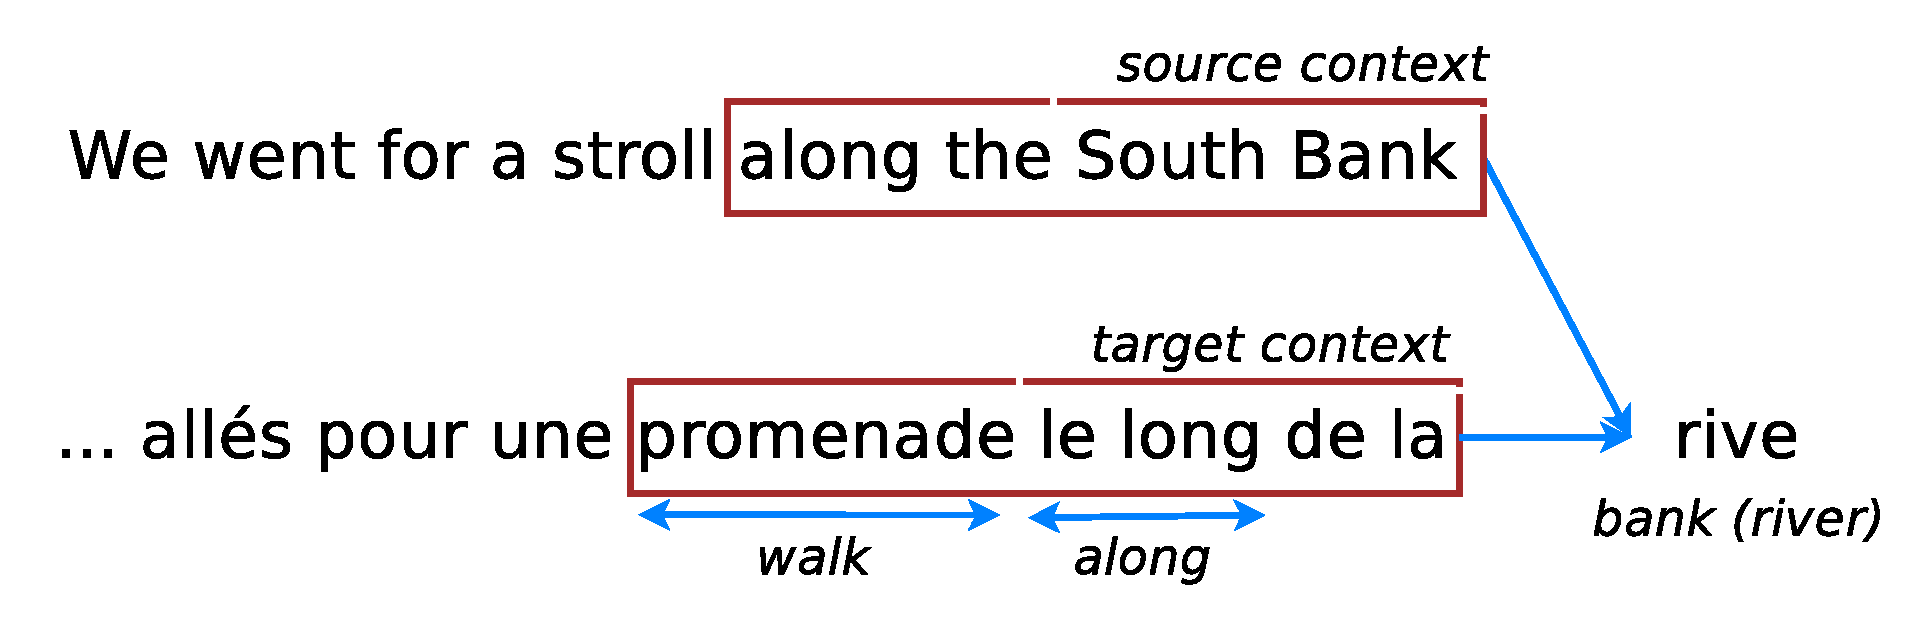
\includegraphics[width=0.7\textwidth, clip=true, trim= 0 0 0 0]{img/nnjm.eps} % , angle=-90
\caption[Source-conditioned \nlmtext{}]{{\bf Source-conditioned \nlmtext{}}
(\nlms{}) -- example of a source-conditioned
\nlm{} proposed by \newcite{devlin14}. To evaluate a how likely a next word
\word{rive} is, the model not only relies on previous target words (context)
\word{promenade le long de la} as in
traditional \nlms{} \cite{Bengio2003}, but also utilizes source context \word{along the
South Bank} to lower uncertainty in its prediction.
} 
\label{f:nnjm}
\end{figure}

These hybrid MT systems with \nlm{} components, while having addressed shortcomings
of traditional phrase-based MT,
still translate locally and fail to capture long-range dependencies. For example, in Figure~\ref{f:nnjm}, the
source-conditioned \nlm{} does not see the word \word{stroll}, or any other words
outside of its fixed context windows, which can be useful in deciding that the
next word should be \word{bank} as in \word{river bank} rather \word{financial
bank}. More problematically, the entire MT pipeline is already complex with
different components needed to be tuned separatedly, e.g., translation models,
language models, reordering models, etc.; now, it becomes even worse as
different neural components are incorporated. Neural Machine Translation to the
rescue!


Neural Machine Translation (NMT) is a new approach to translating text from one
language into another that captures long-range dependencies in sentences and
generalizes better to unseen texts. The core of NMT is a single deep neural
network with hundreds of millions of neurons that learn to directly map source
sentences to target sentences \cite{kal13,sutskever14,cho14}. 
%Despite being relatively new 
%\cite{kal13,sutskever14,cho14}, NMT has already shown promising results,
%achieving state-of-the-art performances for
%several language pairs such as
%English-French \cite{luong15}, English-German
%\cite{jean15,luong15attn,sennrich16mono}, and
%English-Czech \cite{jean15wmt,luong16}. 
This is often referred as the sequence-to-sequence or encoder-decoder
approach.\footnote{\newcite{forcada97} wrote the very first paper on sequence-to-sequence models for translation!}
NMT is appealing since it is conceptually
simple and can be trained
end-to-end. NMT translates as follows: an {\it encoder} reads through the given source
words one by one until the
end, and then, a {\it decoder} starts emitting one target
word at a time until a special end-of-sentence symbol is produced. We illustrate
this process in Figure~\ref{f:nmt}. 
% for the model described in \cite{sutskever14}.

\begin{figure}[tbh!]
\centering
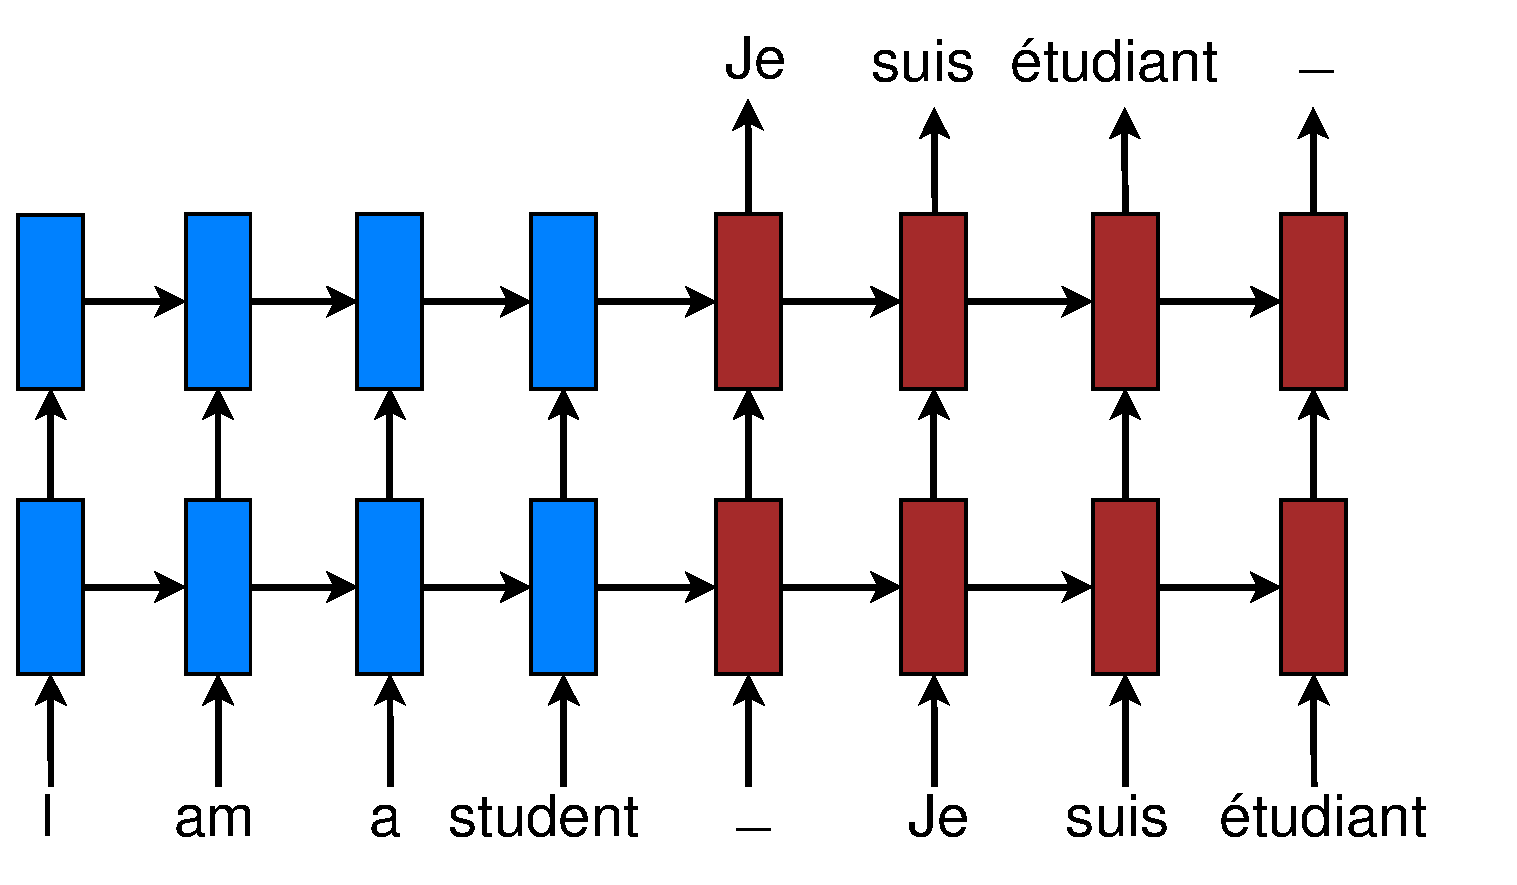
\includegraphics[width=0.6\textwidth, clip=true, trim= 0 0 0
0]{img/nmt_basic.eps} % , angle=-90
\caption[Neural machine translation]{{\bf Neural machine translation} -- example of a deep recurrent
architecture proposed by \newcite{sutskever14} for
translating a source sentence \word{I am a student} into a target sentence
\word{Je suis \'{e}tudiant}. Here, \word{\texttt{\_}} marks the end of a sentence.
} 
\label{f:nmt}
\end{figure}

Such simplicity leads to several advantages. 
NMT requires minimal domain knowledge: it only assumes access to
sequences of source and target words as training data and learns to directly
map one into another. NMT beam-search decoders that
generate words from left to right can be easily implemented, unlike the highly
intricate decoders in standard MT \cite{Koehn:2003:SMT}. Lastly, the use of
recurrent neural networks (RNNs) allow NMT to generalize well to very long word
sequences while not having to 
explicitly store any gigantic
phrase tables or language models as in the case of standard MT.

\section{Thesis Outline}
Despite all the aforementioned advantages and potentials, the early NMT architecture
\cite{sutskever14,cho14} still has many drawbacks. In this thesis, I will
highlight three problems pertaining to the existing NMT model, namely the
{\it vocabulary size}, the {\it sentence length}, and the {\it
language complexity} issues. Each chapter is devoted to solving each of these
problems in which I will describe how I have pushed the limits of NMT, making it
applicable to a wide variety of languages with state-of-the-art performance such as
English-French \cite{luong15}, English-German \cite{luong15attn,luong15iwslt}, and
English-Czech \cite{luong16}. Towards the {\it future} of
NMT, I answer two questions: (1) whether we can improve translation by jointly
learning from a wide variety of sequence-to-sequence tasks such as parsing,
image caption generation, and auto-encoders or skip-thought vectors
\cite{luong16iclr}; and (2)
whether we can compress NMT for mobile devices \cite{see16}.
In brief, this thesis is organized as follows. I start off by providing background knowledge on RNN and NMT
in Chapter~\ref{c:background}. 
The aforementioned three problems and approaches for NMT future are detailed in
Chapters~\ref{c:copy},~\ref{c:attention},~\ref{c:hybrid}, and~\ref{c:future}
respectively, which we will go through one by one next.
%My contributions are detailed in:
%Chapter~\ref{c:copy} on the rare word problem, Chapter~\ref{c:attention} on the
%sentence length problem, Chapter~\ref{c:hybrid} on the language complexity
%problem, and Chapter~\ref{c:future} on the future of NMT.
Chapter~\ref{c:conclude} wraps up and discusses remaining challenges in NMT research.

\subsubsection*{Copy Mechanisms} 
%\paragraph{Copy Mechanisms} 
A significant weakness in conventional NMT 
systems is their inability to correctly translate very rare words:  
end-to-end NMTs tend to have relatively small vocabularies with a single
\unk{} symbol that represents every possible out-of-vocabulary (OOV) word. In
Chapter~\ref{c:copy}, we propose simple and effective techniques to address this
{\it vocabulary size} problem through teaching NMT to ``copy'' words from source to
target. Specifically, we train an NMT system on data that is augmented by the output of a word 
alignment algorithm, allowing the NMT system to emit, for each OOV word
in the target sentence, the position of its corresponding word in the source sentence.
This information is later utilized in a
post-processing step that translates every OOV word using a dictionary.  Our
experiments on the WMT'14 English to French translation task show that this 
method provides a substantial improvement of up to 2.8 BLEU points over an
equivalent NMT system that does not use this technique. 
With 37.5 BLEU points, our NMT system is the first to surpass 
the best result achieved on a WMT'14 contest task.

\subsubsection{Attention Mechanisms} 
%\paragraph{Attention Mechanisms} 
While NMT can translate well for short- and medium-length sentences, it 
has a hard time dealing with long sentences.
An attentional mechanism was proposed by \newcite{bog15} to address that {\it
sentence length} problem by
selectively focusing on parts of the source sentence during translation. However,
there has been little work exploring useful architectures for attention-based
NMT. Chapter~\ref{c:attention} examines two simple and effective classes of attentional
mechanism: a {\it global} approach which always attends to all source words and
a {\it local} one that only looks at a subset of source words at a time. 
We demonstrate the effectiveness of both approaches on the WMT translation
tasks between English and German in both directions. With local
attention, we achieve a significant gain of 5.0 BLEU points over
non-attentional systems that 
already incorporate known techniques such as dropout. Our ensemble 
model using different attention architectures yields a new
state-of-the-art result in the WMT'15 English to German
translation task with 25.9 BLEU points, an improvement of 1.0 BLEU points over the existing
best system backed by NMT and an $n$-gram reranker.

\subsubsection{Hybrid Models} 
%\paragraph{Hybrid Models} 
Nearly all previous NMT work has used quite restricted
vocabularies, perhaps with a subsequent method to patch in unknown words such as
the copy mechanisms mentioned earlier. While effective, the copy mechanims cannot deal with all the
complexity of human languages such as rich morphology, neologisms, and informal
spellings.
Chapter~\ref{c:hybrid} presents a novel word-character solution to that {\it
language complexity} problem towards achieving
open vocabulary NMT.
We build hybrid systems that translate mostly at the {\it word}
level and consult the {\it character} components for rare words. 
Our character-level recurrent neural networks compute source
word representations and recover unknown target words when needed.
The twofold advantage of such a hybrid approach is that it is much faster and easier to
train than character-based ones; at the same time, it never produces unknown words as in the case of word-based models. 
On the WMT'15 English to Czech translation task, 
this hybrid approach offers an addition boost of +$2.1{-}11.4$ BLEU points over models 
that already handle unknown words. 
Our best system achieves a new state-of-the-art result with
$20.7$ BLEU score.
We demonstrate that our character models can successfully learn to not only generate well-formed words for Czech, a
highly-inflected language with a very complex vocabulary, but also build correct
representations for English source words.

\subsubsection{NMT Future} 
%\paragraph{NMT Future} 
Chapter~\ref{c:future} answers the two aforementioned questions
for the future of NMT: whether we can utilize other tasks to improve
translation and whether we can compress NMT models.
%, I answer two questions in Chapter~\ref{c:future}: (1) whether we can improve translation by jointly
%learning from a wide variety of sequence-to-sequence tasks such as parsing,
%image caption generation, and auto-encoders or skip-thought vectors; and (2)
%whether we can compress NMT for mobile devices.

For the first question, 
we examine three multi-task learning (MTL) settings for sequence to sequence
models:
(a) the {\it one-to-many} setting -- where the encoder is shared
between several tasks such as machine translation and
syntactic parsing, (b) the {\it many-to-one} setting -- useful when only the
decoder can be shared, as in the case of 
translation and image caption generation, and (c) the {\it
  many-to-many} setting -- where multiple encoders and decoders are
shared, which is the case with unsupervised objectives
and translation.  Our results show that training on a small amount of parsing and
image caption data can improve the translation quality between English and
German by up to $1.5$ BLEU
points over strong single-task baselines on the WMT benchmarks. Rather
surprisingly,
we have established a new {\it
state-of-the-art} result in constituent parsing with 93.0 F$_1$ by utilizing
translation data. Lastly, we reveal interesting properties of the two unsupervised learning
objectives, autoencoder and skip-thought, in the MTL context: autoencoder helps less in terms of
perplexities but more on BLEU scores compared to skip-thought.

%Neural Machine Translation (NMT), like many other deep learning domains, typically suffers from over-parameterization, resulting in large storage sizes.
For the second question, we examine three simple magnitude-based pruning schemes to compress NMT models, namely {\it class-blind}, {\it class-uniform}, and {\it class-distribution}, which differ in terms of how pruning thresholds are computed for the different classes of weights in the NMT architecture.
We demonstrate the efficacy of weight pruning as a compression technique for a state-of-the-art NMT system. 
We show that an NMT model with over 200 million parameters can be pruned by 40\% with very little performance loss as measured on the WMT'14 English-German translation task. 
This sheds light on the distribution of redundancy in the NMT architecture.
Our main result is that with {\it retraining}, we can recover and even surpass the original performance with an 80\%-pruned model. 


%We start off by providing background knowledge on RNN and NMT
%in Chapter~\ref{c:background}. The following chapters detail my contributions.
%Chapter~\ref{c:copy} discusses how the rare word
%problem in NMT is addressed with a mechanism to ``copy'' words from source to
%target; hence, extending the vocabulary
%coverage. Chapter~\ref{c:attention} describes
%how the attention mechanism, a way to select
%local contexts in the source sentence as we transate, can be effectively used in
%NMT to better handle long sentences. Chapter~\ref{c:hybrid} 
%proposes a novel way of dealing with language complexity (rich morphology,
%neologisms, and informal spellings) by building a hybrid word and character
%level model which can gain from the flexibility of a character-level model while
%maintaining the speed and quality of the word-level model. Towards the future of
%NMT, I answer two questions in Chapter~\ref{c:future}: (1) whether we can improve translation by jointly
%learning from a wide variety of sequence-to-sequence tasks such as parsing,
%image caption generation, and auto-encoders or skip-thought vectors; and (2)
%whether we can compress NMT for mobile devices.
%Chapter~\ref{c:conclude} wraps up and discusses remaining challenges in NMT
%research.


%Due to computational constraint, NMT has to limit its vocabulary to a fixed set
%of top frequent words, e.g., the top 50K words. As a result, all other words
%are represented by a universal symbol \unk{}.
%
%I discuss in Chapter~\ref{c:copy} discusses how the rare word
%problem in NMT is addressed with a mechanism to ``copy'' words from source to
%target; hence, extending the vocabulary
%coverage.



\chapter{Background}
\label{c:background}
\epigraph{For neural machine translation, it all started from language
modeling.}{Thang Luong.}

Language modeling plays an
indispensable role in ensuring that machine translation systems produce fluent target
sentences and has always been an active area of research.
Despite much effort in improving traditional \ngram{} language models
\cite{rosenfeld2000,srilm,teh2006,irstlm,kenlm,pauls2011,heafield13},
traditional LMs inherently can only handle short
contexts of a few words. Approaches to building \nlmtext{} (\nlms) using
feed-forward networks such as those initiated by \newcite{Bengio2003} and
enhanced by others \cite{Morin2005,Bengio08,MnihHinton2009,MnihTeh2012} have %,Mnih2007
addressed that drawback to model longer contexts.
% worked great compared to traditional \ngram{} language models. 
Still, \nlms{} can only capture fixed-length contexts and is
incapable of handling variable-length sequences, which is the case for sentences.
Recurrent neural networks (RNNs) come in handy as a powerful and expressive
architecture to handle sequential data and have successfully been applied to the
language modeling task \cite{MikolovKBCK10,MikolovKBCK11,mikolovLM}.
By viewing RNNs as generative models \cite{Sutskever11} that can produce texts 
and by pushing another step towards conditioning RNNs on source sentences, recent works
\cite{kal13,sutskever14,cho14} have started a new line of resesarch in machine translation, namely Neural
Machine Translation (NMT). NMT is technically a source-conditioned \nlm{} that
can be trained end-to-end.

%Early success of feed-forward \nlms{} has led to widespread adoption of \nlms{}
%as an additional component in the machine translation pipeline
%such as \cite{schwenk07,vaswani13decode,luong15nlm}, inter alia.
%\cite{Schwenk12continuous,Son:2012:CST,Auli13,devlin14}

%An important part in the machine translation pipeline is the ability to model language
%coherence at the target side. 
%As such, a significant amount of effort in
%improving MT has centered around enhancing language modeling -- more specifically, the need to capture long-range
%dependencies better. We start out with efforts to scale up traditional \ngram{} language models 

In this chapter, we provide background knowledge on two main topics, RNN and NMT.
We first go through the basics of RNNs, explaining how they can be used to model sentences. 
Then, we delve into details of one particular type of RNNs, the Long Short-term Memory, that makes training RNNs easier.
Given RNNs as a building block, we discuss NMT together with tips and tricks for better training and testing NMT.

\section{Recurrent Neural Network}
Recurrent Neural Network (RNNs) \cite{elman90} are models that help understand
the temporal aspect as well as build up representations for sequential data
using a dynamic memory structure. At the surface form, an RNN takes as input a sequence of vectors $\x{1},
\x{2}, \ldots, \x{n}$ and processes them one by one. For each
new input $\x{i}$, an RNN updates its memory to produce a hidden state
$\hid{i}$ which one can think of as a representation for the partial sequence
$\x{\overline{1,i}}$. %$\x{1},\ldots, \x{i}$. 
The beauty of RNNs lies in the fact that it can
capture the dynamics of an arbitrarily long sequence without having to increase its modeling
capacity unlike the case of feedforward network which can only model
relationship within a fixed-length sequence. The key secret sauce is in the
recurrence formula of an RNN that defines how its hidden state is updated. At
its simplest form, a ``vanilla'' RNN defines its recurrence function as:
\begin{align}
\hid{t} &= f\paren{\x{t}, \hid{t-1}} \label{e:abstract_rnn}
\end{align}
In the above formula, $f$ is an abstract function that computes a new hidden state given the current input $\x{t}$ and the
previous hidden state $\hid{t-1}$. The starting state $\hid{0}$ is often set to
$\bm{0}$ though it can take any value as we will see later in the context
of NMT decoders. A popular choice of $f$ is provided below with $\sigma$ being a
non-linear function such as $\sigmoid$ or $\tanh$.\footnote{There could also be
an optional bias term in \eq{e:vanilla_rnn}.}
\begin{align}
%\z{t} &= \W{xh}\x{t} + \W{hh}\hid{t-1} \label{e:vanilla_rnn} \\
\hid{t} &= \sigma(\W{xh}\x{t} + \W{hh}\hid{t-1} \label{e:vanilla_rnn}) %\z{t})
\end{align}

At each timestep $t$, an RNN can (optionally) emit an output symbol
$y_t$ which can either be discrete or real-valued. For the discrete scenario,
which is often the case for languages, a probability distribution $\bm{p}$ over a 
set of output classes $Y$ is derived as
follows\footnote{For the real-valued case, we refer readers to mixture density
models \cite{bishop94} which have been applied to RNN training, e.g., for
hand-writing synthesis \cite{graves13c}.}:
\begin{align}
\s{t} &= \W{hy}\hid{t} \label{e:score} \\
\prob{t} &= \softmax(\s{t}) \label{e:prob}
\end{align}
Here, we introduce a new set of weights $\W{hy} \inR{|Y| \times d}$, with $d$ being the dimension of the RNN hidden
state, to compute a score vector $\s{t}$, or {\it logits}, over
different individual classes. Often, with a large output set $Y$, the
matrix-vector multiplication in \eq{e:score} is a major computational
bottleneck in RNNs, which results in several challenges for neural language modeling
and machine translation that we will address in later chapters. 
The $\softmax$ function transforms the score
vector $\s{t}$ into a probability vector $\prob{t}$, which is defined for each specific
element $y \in Y$ as below.
For convenience, we overload our notations to use $\prob{t}(y)$ and $\s{t}(y)$ to refer to entries in
the vectors $\prob{t}$ and $\s{t}$ that correspond to $y$.
\begin{align}
\prob{t}(y) = \frac{\e^{\s{t}(y)}}{\sum_{y' \in Y} \e^{\s{t}(y')}}
\label{e:softmax}
\end{align}

With the above formulae, we have completely defined the RNN weight set $\thetav$
%=\!\{\W{xh}, \W{hh}, \W{hy}\}$, 
which consists of {\it input} connections $\W{xh}$, {\it
recurrent} connections $\W{hh}$, and {\it output}
connections $\W{hy}$. These weights are shared across
timesteps as illustrated in Figure~\ref{f:rnn} \error{Draw a picture on
general RNNs}, which enables
RNNs to handle arbitrarily long sequences.

\begin{figure}[tbh!]
\centering
%\psgrid
\rput(7.1,2.6){{\color{lightblue} $\MB{W_{hh}}$}}
\rput(8.6,1.0){{\color{lightgreen} $\MB{W_{xh}}$}}
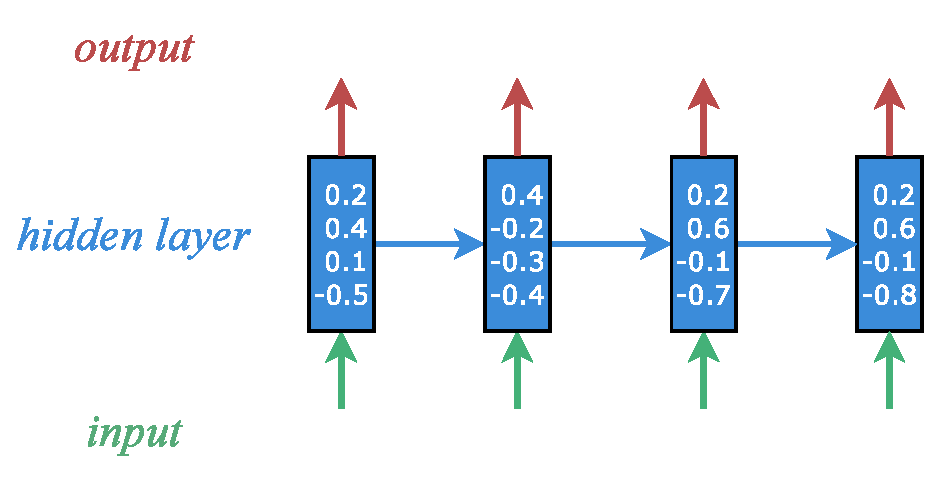
\includegraphics[width=0.6\textwidth, clip=true, trim= 0 0 0 0]{img/rnn.eps} % , angle=-90
\caption[Recurrent neural networks]{{\bf Recurrent neural networks} -- example of a recurrent
neural network that processes a sequence of input words \word{I am a student} to
build up hidden representations as input symbols are consumed. The recurrent
$\MB{W_{hh}}$ and feed-forward $\MB{W_{xh}}$ weights are shared across
timesteps.
} 
\label{f:rnn}
\end{figure}

Next, we discuss the training and testing phases of RNNs from a slightly more
focused angle, the language learning aspect. For more details on RNNs, we refer readers to the following resources
\cite{sutskever12,mikolov12,karpathy15rnn}.

\subsection{Recurrent Language Models}
To apply RNNs to sentences in languages, or generally sequences of discrete symbols, one can
consider one-hot representations $\x{i} \inR{|V|}$, with $V$ being the
vocabulary considered. However, for a large
vocabulary $V$, such a representation choice is problematic as it results in
a large weight matrix $\W{xh}$ and there is no notion of similarity between
words. In practice, low-dimensional dense representations for words, or {\it
word embeddings}, are often used to address these problems. Specifically, an
embedding matrix
$\W{e} \inR{d_e \times |V|}$ is looked up for each word $x_i$ to retrieve a
representation $\x{i} \inR{d_e}$. As a result, a simple RNN applied to language
modeling will generally have $\theta = \{\W{xh}, \W{hh}, \W{hy}, \W{e}\}$ as its
weights as illustrated in Figure~\ref{f:rlm} \error{Draw an RNN with
embedding}.

\begin{figure}[tbh!]
\centering
%\psgrid
\rput(7.1,2.6){{\color{lightblue} $\MB{W_{hh}}$}}
\rput(8.6,1.0){{\color{lightgreen} $\MB{W_{xh}}$}}
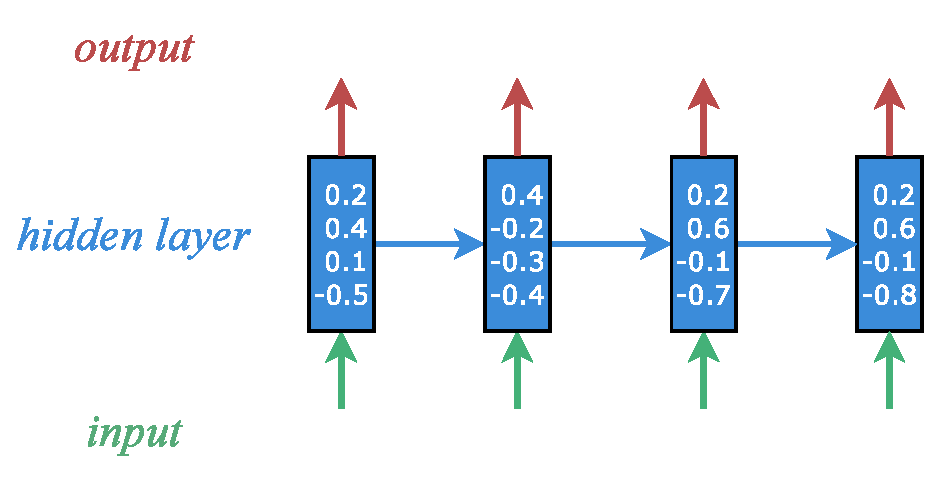
\includegraphics[width=0.6\textwidth, clip=true, trim= 0 0 0 0]{img/rnn.eps} % , angle=-90
\caption[Recurrent language models]{{\bf Recurrent language models} -- example of a recurrent
neural network that processes a sequence of input words \word{I am a student} to
build up hidden representations as input symbols are consumed. The recurrent
$\MB{W_{hh}}$ and feed-forward $\MB{W_{xh}}$ weights are shared across
timesteps.
} 
\label{f:rlm}
\end{figure}

In language modeling (LM), the task is to specify a probability distribution over
sequences of symbols (often, words) so that one can judge if a sequence of
words is more likely or ``fluent'' than another. To accomplish that, an LM decomposes the
probability of a word sequence $y = y_1, \ldots,
y_m$ as:
\begin{align}
p(y) = \prod_{i=1}^m p(y_i | y_{<i}) %\yrange{1}{i-1})
\end{align}
In the above formula, each of the
individual term $p(y_i | y_{<i})$ is the conditional probability of the current
word $y_i$ given previous words $y_{<i}$, also referred as the {\it
context} or the {\it history}. To model these conditional probabilities, traditional \ngram{}
as well as feedforward-based neural language models have to resort to the
Markovian assumption to model only a fixed window of context, i.e., $p(y_i |
y_{i-n+1}, \ldots, y_{i-1})$. An RNN-based language model naturally lends itself to model the full
history as we shall see now.

An RNN-based language model (RNNLM) is a special case of RNNs in which: (a) the input and output
are sequences of discrete words, (b) the output sequence ends %$y=\{y_1, \ldots, y_n$, \eos$\}$ 
with a special symbol \eos{} that marks the boundary, e.g., $y=\{$ ``I'', ``am'', ``a'',
``student'', \eos$\}$, and (c) the input sequence is a
shift-by-1 version of the output sequence with \sos{} as a starting symbol,
e.g., $x=\{$ \sos, ``I'', ``am'', ``a'',
``student''$\}$. We illustrate this in \figref{f:rlm}.

%i.e., $x=\{$
%\sos{}, $y_1, \dots, y_n\}$. In our example, $x=\{$ \sos, ``I'', ``am'', ``a'',
%``student''$\}$, whereas $y=\{$ ``I'', ``am'', ``a'',
%``student'', \eos$\}$
\paragraph{Training}
Given a training dataset of $N$ discrete output sequences $\ytop{1}, \ldots,
\ytop{N}$ with lengths $m_1, \ldots, m_N$ accordingly. The learning objective is
to minimize the negative log-likelihood, or the {\it cross-entropy} loss, of these training examples:
\begin{align}
J(\thetav) &= \sum_{i=1}^{N} -\log p\paren{\ytop{i}} \\ 
&= \sum_{i=1}^{N} \sum_{t=1}^{m_i} -\log p\paren{\ytop{i}_t |
\ytop{i}_{<t}}
\end{align}

RNN learning is often done using mini-batch stochastic gradient descent (SGD) algorithms in
which a small set of training examples, a {\it mini-batch}, is used to compute
the gradients and update weights one at a time. Using mini-batches has
several advantages: (a) the gradients are more reliable and consistent than the
``online'' setting which updates per example, (b) less computation is required to
update the weights unlike the case of full-batch learning which has to process
all examples before updating, and (c) with multiple examples in a mini-batch,
one can turn matrix-vector multiplications such
as those in \eq{e:vanilla_rnn} and \eq{e:score} into matrix-matrix multiplications which can be
deployed efficiently on GPUs. The simplest weight update formula with $\eta$ as
a learning rate is given below:
\begin{align}
\thetav \longleftarrow \thetav - \eta \grad{J(\thetav)} %\fracder{J(\thetav)}{\thetav}
\end{align}

\paragraph{Single-timestep Backpropagation} To compute the gradients for the loss $J(\thetav)$,
we first need to be able to derive the gradients of the per-timestep loss $l_t
=\log \prob{t}(y_t)$ with respect to both the RNN weights
$\{\W{xh}, \W{hh}, \W{hy}\}$ and the inputs $\{\x{t}, \hid{t-1}\}$. We denote
these gradients as $\{d\W{xh}, d\W{hh}, d\W{hy}, d\x{t}, d\hid{t-1}\}$
respectively and define intermediate gradients $d\s{t}, d\hid{t}$ similarly. 
Starting with the loss $l_t$, we employ backpropagation through structures
\cite{goller:ieeenn00} to derive each gradient one by one in the following
order: $l_t \rightarrow \s{t} \rightarrow \{\hid{t}, \W{hy}\} \rightarrow
\{\x{t}, \hid{t-1}, \W{xh}, \W{hh}\}$.
First, from \eq{e:softmax}, we have:
\begin{align}
d\s{t} = \fracder{\l_t}{\s{t}} = \parfrac{\s{t}} \paren{\s{t}(y_t) - \log \sum_{y'}
e^{\s{t}(y')}}
\end{align}

Computing per-coordinate gradient $\s{t}(y)$ gives:
\begin{align}
 \parfrac{\s{t}(y)} \paren{\s{t}(y_t) - \log \sum_{y'} e^{\s{t}(y')}} =
  \begin{cases}
   1 - \prob{t}(y_t) & y = y_t \\
   -\prob{t}(y) & y \neq y_t
  \end{cases}
\end{align}

The above gradients can be concisely written in vector form as:
\begin{align}
d\s{t} = \bm{1}_{y_t} - \prob{t}
\end{align}

Here, $\prob{t}$ is the probability distribution defined in \eq{e:prob} and has been calculated in the forward pass,
so we simply reuse it. $\bm{1}_{y_t}$ is a one-hot vector with 1 at position
$y_t$. 
Applying Corollary~\ref{c:chain_rule}, noting that $\s{t} = \W{hy}\hid{t}$ in \eq{e:score}, we
arrive at:
\begin{align}
% h_t
d\hid{t} &=  \tp{\W{hy}} \cdot d\s{t}\\
% W_hy
d\W{hy} &=  d\s{t} \cdot \tp{\hid{t}}
\end{align}

At this point, we have derived part of the backpropation procedure which can be
applied to any hidden unit type, e.g., the aforementioned vanilla RNN or the
LSTM unit that we will describe shortly in the next section. 

{\it Vanilla RNN Backpropagation} \indent 
%For the vanilla RNN formulation in \eq{e:vanilla_rnn}, we further backpropagate
%the loss as follows.
%For simplicity and convenience, one can set the embedding size to be equal to the
%hidden size, so $\W{xh}, \W{hh} \inR{d \times d}$. We can further 
First of all, we can simplify the notation to have $\rnn\!=\![\MB{W_{xh}}
\MB{W_{hh}}]$ and $\z{t}\!=\![\x{t};
\hid{t-1}]$, so the RNN formulation in \eq{e:vanilla_rnn} % \inR{2d}
becomes:
\begin{align}
\MB{h_t} = \sigma \paren{\rnn \z{t}}
\end{align}

Applying \lemmaref{l:chain_rule}, we have:
\begin{align}
% z_t
d\z{t} &=  \tp{\rnn} \cdot
\paren{\sigma'(\rnn \z{t}) \odot d\hid{t}} \label{e:grad_zt} \\
% T_dx2d 
d\rnn &=  \paren{\sigma'(\rnn \z{t}) \odot d\hid{t}} \cdot \tp{\z{t}} \label{e:grad_rnn}
\end{align}

This is one of the {\it tricks} that we use to better utilize GPUs by creating
larger matrices and vectors, i.e., $\rnn$ and $\z{t}$. From \eq{e:grad_zt} and
\eq{e:grad_rnn}, one can easily extract the following gradients:
(a) $d\x{t}$ -- embedding gradients which we use to sparsely update the embedding weights $\W{e}$, (b) $d\hid{t-1}$
 -- gradients of the previous hidden state, which is needed by the
 backpropagation-through-time algorithm that we will discuss next, and (c) $d\W{xh}$ as well
as $d\W{hh}$ -- the RNN input and recurrent connections.\footnote{One can also
separately derive these gradients as follows:
\begin{align*}
% x_t
d\x{t} &=  \tp{\W{xh}} \cdot \paren{\sigma'(\rnn \z{t}) \odot d\hid{t}}\\
% h_{t-1}
d\hid{t-1} &=  \tp{\W{hh}} \cdot \paren{\sigma'(\rnn \z{t}) \odot d\hid{t}}\\
% W_xh 
d\W{xh} &=  \paren{\sigma'(\rnn \z{t}) \odot d\hid{t}} \cdot \tp{\x{t}} \\
% W_hh 
d\W{hh} &=  \paren{\sigma'(\rnn \z{t}) \odot d\hid{t}} \cdot \tp{\hid{t-1}}
\end{align*}
}

\paragraph{Backpropagation Through Time (BPTT)}
Having defined a single-timestep backpropagation procedure, we are now ready to
go through the BPTT algorithm \cite{Rumelhart:1986:LPT,werbos1990}. Inspired by 
\newcite{sutskever12}, we summarize the BPTT algorithm for RNNs below with the
following remarks: (a) Lines 3, 5, 6, 7 accumulate the gradients of RNN weights
$\{\W{hy}, \W{xh}, \W{hh}, \W{e}\}$ over time; (b) In line 7, $d\x{t}$ refers to
gradients of words participating in the current mini-batch which we use to
sparsely update $\W{e}$;\footnote{In multi-layer
RNNs, $d\x{t}$ is used to send gradients down to the below layers.} and (c) Line
4 accumulates gradients for the current hidden state $\hid{t}$ by considering two paths,
a ``vertical'' one from  the current loss at time $t$ and a ``recurrent'' one from the timestep
$t+1$ which was set in Line 8 earlier.

\begin{algorithm}
\For{$t=T \rightarrow 1$}
{
\tcp{Output backprop}
% d_s
$d\s{t} \leftarrow \bm{1}_{y_t} - \prob{t}$

% W_hy
$d\W{hy} \leftarrow d\W{hy} + d\s{t} \cdot \tp{\hid{t}}$

% h_t
$d\hid{t} \leftarrow d\hid{t} + \tp{\W{hy}} \cdot d\s{t}$

\tcp{RNN backprop}
% W_xh 
$d\W{xh} \leftarrow d\W{xh} + \paren{\sigma'(\rnn \z{t}) \odot d\hid{t}} \cdot \tp{\x{t}}$

% W_hh 
$d\W{hh} \leftarrow d\W{hh} + \paren{\sigma'(\rnn \z{t}) \odot d\hid{t}} \cdot \tp{\hid{t-1}}$

\tcp{Input backprop}
% x_t
$d\x{t} \leftarrow \tp{\W{xh}} \cdot \paren{\sigma'(\rnn \z{t}) \odot d\hid{t}}$

% h_{t-1}
$d\hid{t-1} \leftarrow \tp{\W{hh}} \cdot \paren{\sigma'(\rnn \z{t}) \odot d\hid{t}}$
}
\caption{BPTT algorithm for ``vanilla'' RNNs}
\end{algorithm}

\subsection{Better Training RNNs}
%For simplicity and convenience, one can set the embedding size to be equal to the
%hidden size, so $\W{xh}, \W{hh} \inR{d \times d}$. We can further simplify the
%notation to have $\rnn = [\MB{W_{xh}} \MB{W_{hh}}]$, so \eq{e:vanilla_rnn}
%becomes:
%\begin{align}
%\MB{h_t} = \sigma \paren{\rnn
%\begin{bmatrix}
%  \MB{x_t} \\
%  \MB{h_{t-1}}
% \end{bmatrix}
%}
%\end{align}


%\paragraph{Exploding and Vanishing Gradients}
Even though computing RNN gradients is straightforward once 
the BPTT algorithm has been plotted out, training is inherently difficult due to the nonlinear
iterative nature of RNNs. Among all reasons, 
the two classic problems of RNNs that often arise when dealing with very long sequences are the {\it
exploding} and {\it vanishing} gradients as
described by \newcite{Bengio-trnn94}. In short, exploding gradients refer to the
phenomenon that the gradients become exponentially large as we backpropagate
over time, making learning unstable. Vanishing gradients, on the
other hand, is the opposite problem when the gradients go exponentially fast
towards zero, turning BPTT into truncated BPTT that is unable to capture long-range
dependencies in sequences. 

Let us try to explain the aforementioned problems informally and 
refer readers to more rigorous and in-depth analyses in \cite{Bengio-trnn94,lstm97,MartensS11,pascanu13}.
The main cause of these two problems all lies in Line 8 of the BPTT
algorithm, in which we can rewrite the assignment as
$d\hid{t-1} = \tp{\W{hh}} \cdot \diag\paren{\sigma'(\rnn \z{t})} \cdot
d\hid{t}$. We can try to understand the behavior of RNNs over time by assuming
no contribution of the intermediate losses in Line 4
for a moment. Given such an assumption, a signal sent from the current hidden state over K
steps will become 
$d\hid{t-K} = \prod_{i=1}^{K} \paren{\tp{\W{hh}} \cdot \diag\paren{\sigma'(\rnn
\z{t-i+1})}} \cdot
d\hid{t}$. Assuming that the non-linear function $\sigma$ is bounded, e.g.,
$\sigm$ and $\tanh$, and behaves ``nicely'', what we need to deal with now is
the multiplication of the recurrent matrix over time.
This leads to the fact that the behavior of RNNs is often governed by the characteristics of the recurrent matrix
$\W{hh}$ and most analyses examine in terms of the largest eigen value of
$\W{hh}$ as well as the norms of these signals. Roughly speaking, if the largest eigen value
is large enough, exploding gradients will be likely to happen. On the contrary,
if the largest eigen value is below a certain threshold, vanishing gradients
will occur as clearly explained by \newcite{pascanu13}.

\error{Discuss LSTM}
\begin{align}
\MB{h}_t = \sigma \paren{
\MB{W_{xh}}\MB{x}_t + \MB{W_{hh}}\MB{h}_{t-1}
}
\end{align}

\begin{align}
\fracder{\MB{h}_t}{\MB{h}_{t-1}} = \diag\paren{\sigma'(\ldots)}\tp{\MB{W_{hh}}}
\end{align}

\begin{align}
\norm{\fracder{\MB{h}_t}{\MB{h}_{t-1}}} & \leq \norm{\diag\paren{\sigma'(\ldots)}} 
\norm{\tp{\MB{W_{hh}}}} \\ 
& \leq \gamma \lambda_1
\end{align}

\begin{align}
\norm{\fracder{\MB{h}_t}{\MB{h}_{t-k}}} \leq \paren{\gamma \lambda_1}^{k}
\rightarrow 0 & \quad \text{ if } \lambda_1 < \frac{1}{\gamma}
\end{align}

\begin{align}
\fracder{\MB{c}_t}{\MB{c}_{t-1}} = \MB{I}
\end{align}

\paragraph{Long Short-Term Memory}
We use the formulation of \cite{zaremba14}.
For a single LSTM block at layer $l$ and time $t$, the new hidden state $\hlt$ and memory cell $\clt$ are calculated from $\MB{h_t^{l-1}}$, $\MB{h_{t-1}^l}$ and $\MB{c_{t-1}^l}$ like so:
\begin{align}
\label{eqn:LSTMdef1}
\begin{pmatrix}
\ilt \\
\flt \\
\olt \\
\glt
\end{pmatrix}
&= 
\begin{pmatrix}
\sigm \\
\sigm \\
\sigm \\
\tanh
\end{pmatrix}
\lstm
\begin{bmatrix}
  \MB{h_t^{l-1}} \\
  \MB{h_{t-1}^l}
 \end{bmatrix} \\
\clt &= \flt \circ \MB{c_{t-1}^l} + \ilt \circ \glt \\
\hlt &= \olt \circ \tanh(\clt)
\end{align}
where $\sigm$ and $\tanh$ are applied element-wise, $\circ$ denotes element-wise multiplication, 
and $\MB{T}_{4n \times 2n}$ is a $4n \times 2n$ matrix of weights that depends on $l$ but not $t$.\footnote{Note: Sometimes these equations are written omitting the superscript $l$ and writing $\MB{h_t^{l-1}}$ as $x_t$, but for the purposes of deriving the back-propagation equations, we need to refer to the layer $l$ explicitly.}
If $l=1$ then $\MB{h_t^{l-1}}$ is the input vector $x_t$.
If $t=1$ then $\MB{h_{t-1}^l}$ and $\MB{c_{t-1}^l}$ are taken to be zero.

An LSTM block at layer $l \in \{1, \dots L\}$ and time $t \in \{1, \dots T\}$ consists of:
\begin{itemize}
\item The hidden state $\hlt \in \mathbb{R}^n$
\item The memory cell $\clt \in \mathbb{R}^n$
\item The input gate $\ilt \in [0,1]^n$
\item The forget gate $\flt \in [0,1]^n$
\item The output gate $\olt \in [0,1]^n$
\item The input modulation gate $\glt \in [0,1]^n$
\end{itemize}
We call $n$ the LSTM block size.

\paragraph{LSTM Backpropation}
$\MB{\delta_{c^{(2)}}}$

$\MB{\delta_{h^{(2)}}}$

$\MB{\delta_{c^{(1)}}}$

$\MB{\delta_{h^{(1)}}}$

$\MB{\delta_{c}} \pluseq \MB{\delta_{h}}\MB{o_t}\tanh'(\MB{c_t}) $

$\MB{\delta_{c}} = \MB{\delta_{c}} \circ \MB{f_t} $

$\MB{\delta_{h}} \pluseq \text{upper grad}$


\section{Neural Machine Translation}
\begin{figure}[tbh!]
\centering
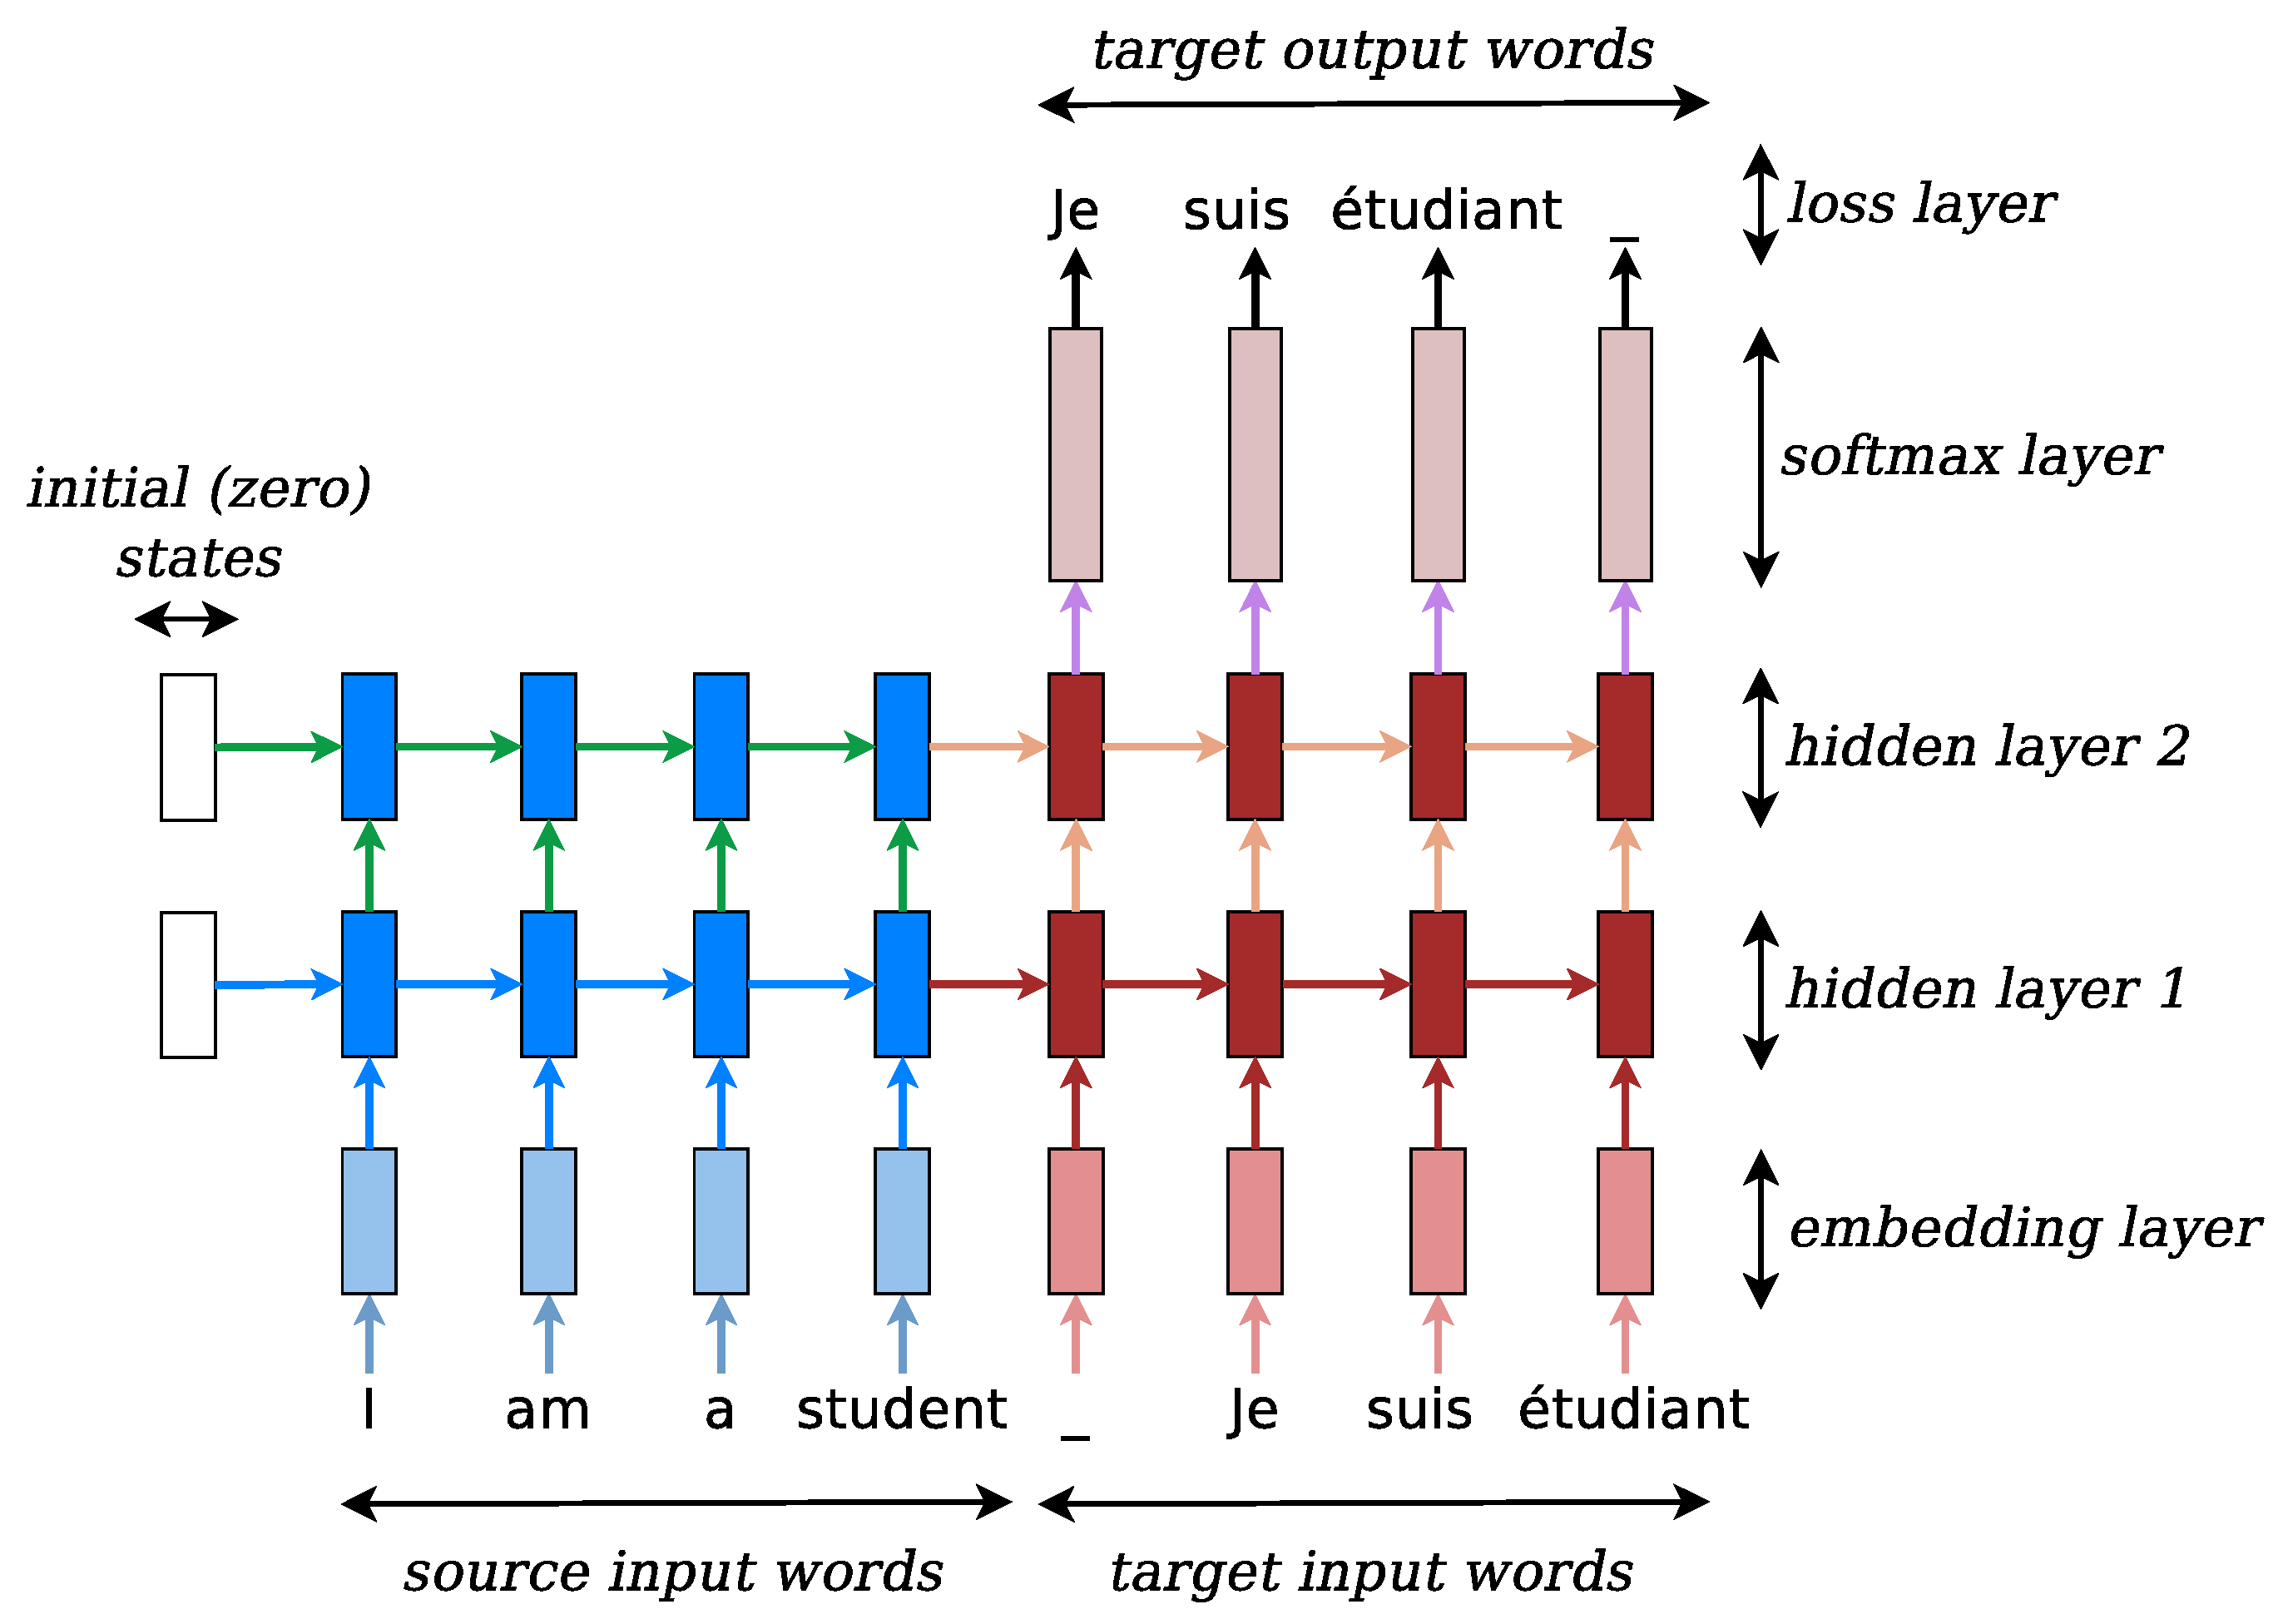
\includegraphics[width=0.8\textwidth, clip=true, trim= 0 0 0
0]{img/nmt_very_details.eps} % , angle=-90
\caption[Neural machine translation]{{\bf Neural machine translation} -- example of a deep recurrent
architecture proposed by \newcite{sutskever14} for
translating a source sentence \word{I am a student} into a target sentence
\word{Je suis \'{e}tudiant}. Here, \word{\texttt{\_}} marks the end of a sentence.
} 
\label{f:nmt_details}
\end{figure}


Neural machine translation aims to directly model the conditional probability $p(\tgt{}|\src{})$ of translating
a source sentence, $\src{1},\ldots,\src{n}$, to a target sentence, $\tgt{1},\ldots,\tgt{m}$.
It accomplishes such goal through the {\it encoder-decoder} framework \cite{sutskever14,cho14}. The {\it encoder} computes a representation $\MB{s}$
for each source sentence. Based on that source representation,
the {\it decoder} generates a translation, one target word at a time, and hence, decomposes the conditional probability as:
\begin{equation}
\log p(\tgt{}|\src{}) = \sum_{j=1}^m \nolimits \log
p\paren{\tgt{j}|\tgt{<j},\src{},\MB{s}}
\end{equation}

A natural choice to model such a decomposition in the decoder is to use a
recurrent neural network (RNN) architecture, which most of the recent NMT work have in common. They,
however, differ in terms of the RNN architectures used and how the encoder computes the source representation $\MB{s}$.
%, e.g., vanilla RNN, long-short term memory (LSTM) \cite{lstm97} or gated recurrent units \cite{cho14}

Kalchbrenner and Blunsom \cite{kal13} used an RNN with the vanilla RNN unit for the decoder and a
convolutional neural network for encoding the source. On
the other hand, Sutskever et al. \cite{sutskever14} and Luong et al.
\cite{luong15,luong15attn} built deep RNNs with the Long Short-Term Memory (LSTM) unit
\cite{lstm97} for both the encoder and the decoder. Cho et al., \cite{cho14}, Bahdanau et al.,
\cite{bog15}, and Jean et al. \cite{jean15,mono15} all adopted an
LSTM-inspired hidden unit, the gated recurrent unit (GRU), and used bidirectional
RNNs for the encoder.
%\footnote{They all used a single RNN layer except for the latter two
%works which utilized a bidirectional RNN for the encoder.}

In more details, considering the top recurrent layer in a deep RNN architecture, one can compute the probability of decoding each target word $y_j$ as:
\begin{equation}
p\left(\tgt{j}|\tgt{<j},\src{},\MB{s}\right) = \softmax\paren{\hd{j}}
\end{equation}
%with $g$ being the transformation function that outputs a vocabulary-sized
%vector.\footnote{One can provide $g$ with other inputs such as the currently
%predicted word $\tgt{j}$ as in \cite{bog15}.} 
with $\hd{j}$ being the current target hidden state computed as:
\begin{equation}
\label{e:rnn}
\hd{j} = f(\hd{j-1}, \tgt{j-1}, \MB{s})
\end{equation}
Here, $f$ derives the current state given the previous state
$\hd{j-1}$, the
current input (often the previous word $\tgt{t-1}$), and optionally, the source
representation $\MB{s}$.
$f$ can be a vanilla RNN unit, a GRU, or an LSTM. 
The early NMT approach  \cite{kal13,sutskever14,cho14,luong15} uses the last source hidden state
$\MB{s}=\hb{n}$ once to initialize the decoder hidden state and sets $\MB{s}=[\text{ }]$ in
\eq{e:rnn}.

\subsection{Training}
The training objective is formulated as follows:
\begin{equation}
J = \sum_{(\src{},\tgt{}) \in \mathbb{D}} \nolimits -\log p(\tgt{}|\src{})
\label{e:j_t}
\end{equation}
with $\mathbb{D}$ being our parallel training corpus.

mention bucketing and batching

\subsection{Testing}

mention beam-search, ensemble

\begin{figure}[tbh!]
\centering
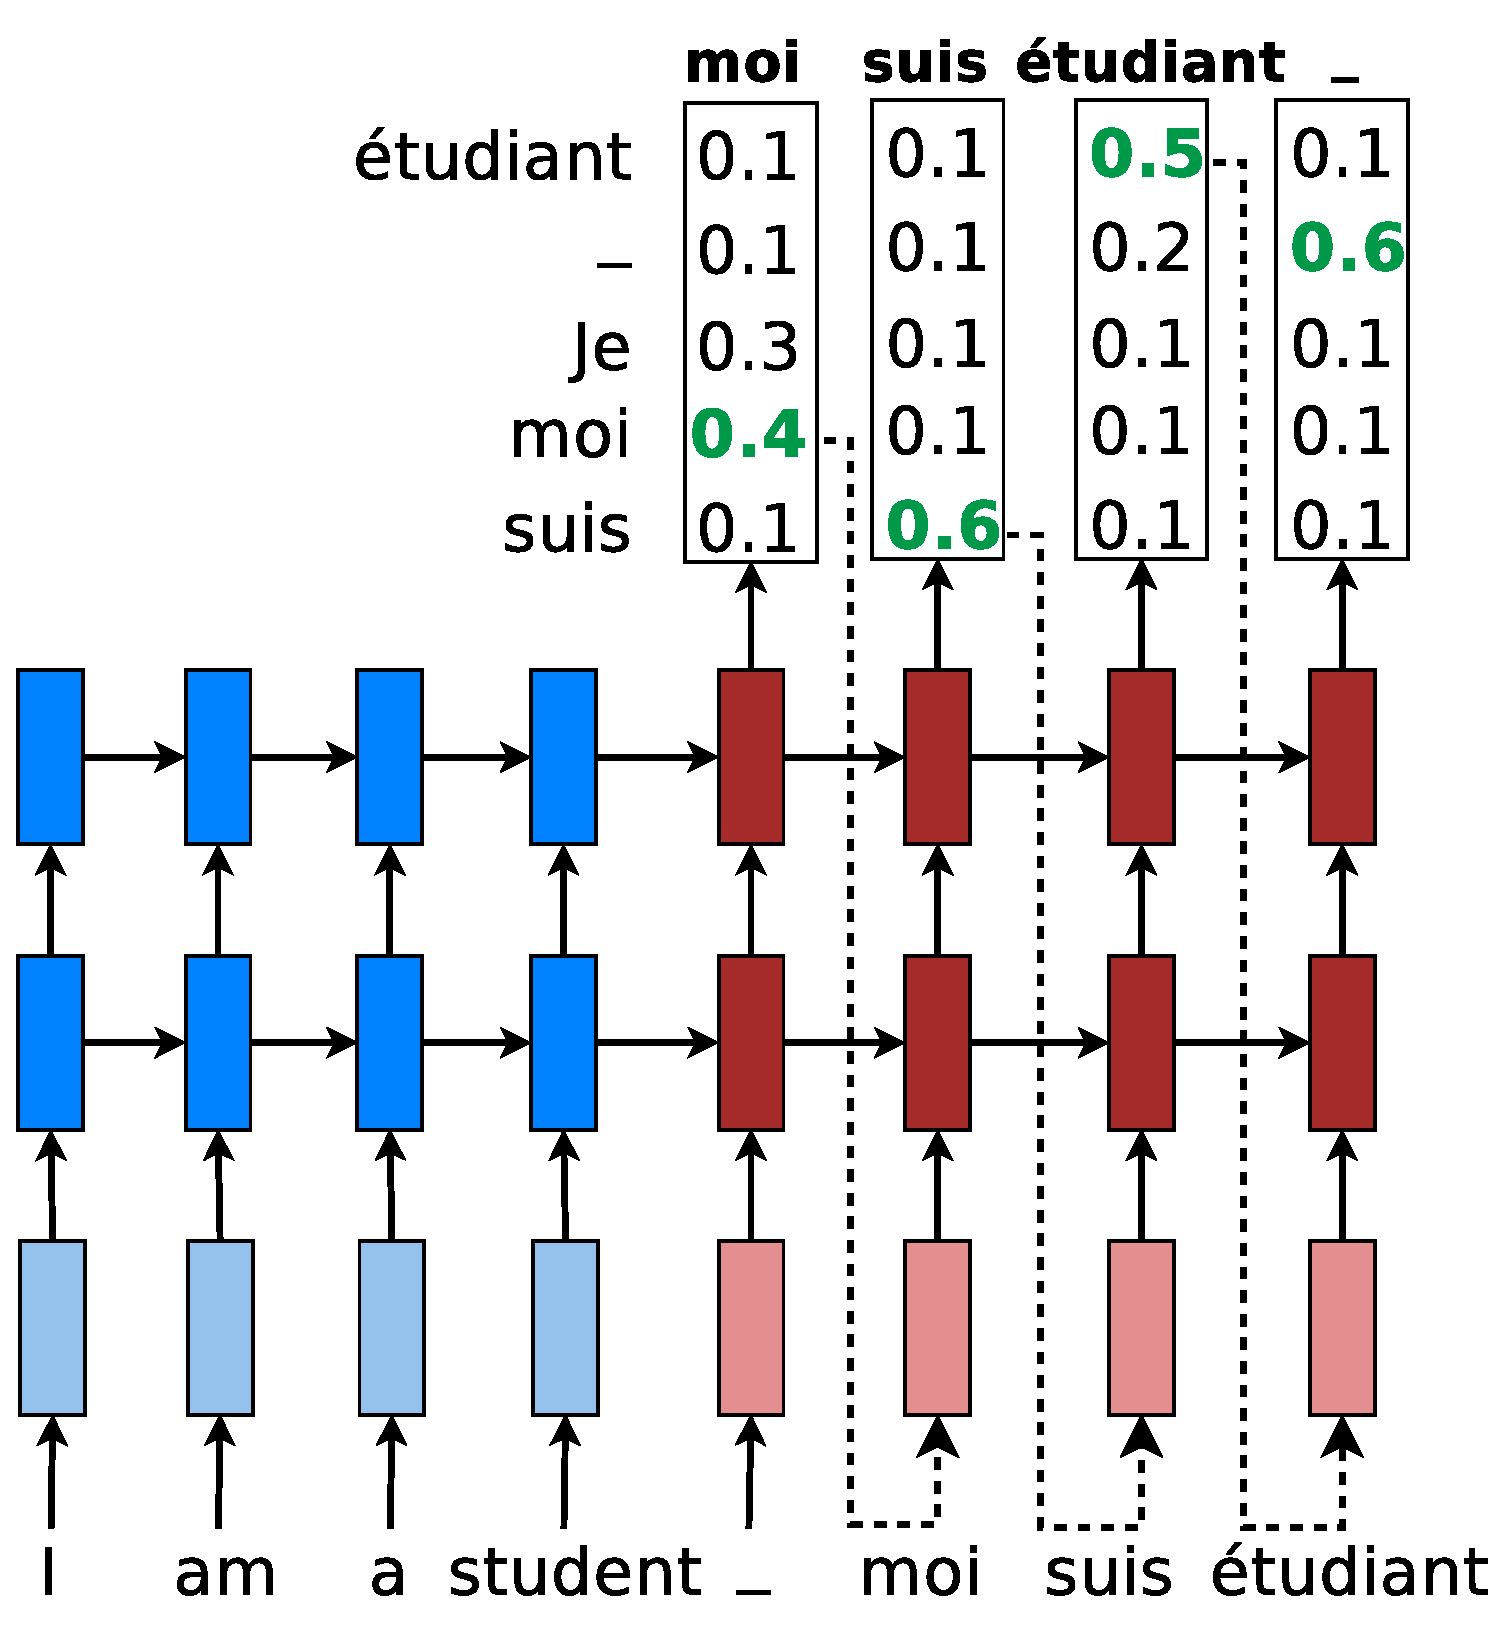
\includegraphics[width=0.6\textwidth, clip=true, trim= 0 0 0
0]{img/nmt_test.eps} % , angle=-90
\caption[Neural machine translation]{{\bf Neural machine translation} -- example of a deep recurrent
architecture proposed by \newcite{sutskever14} for
translating a source sentence \word{I am a student} into a target sentence
\word{Je suis \'{e}tudiant}. Here, \word{\texttt{\_}} marks the end of a sentence.
} 
\label{f:nmt_details}
\end{figure}


%\section{Backward Propagation}
%\subsection{Definitions}
In this section we define some additional notation that will help us to derive the necessary back-propagation equations.

\begin{definition}
Let $U$ and $V$ refer to the $n \times n$ weight matrices corresponding to the following portions of $\MB{T}_{4n \times 2n}$:
\begin{equation}
\MB{T}_{4n \times 2n} = 
\begin{bmatrix}
U_i & V_i \\
U_f  & V_f\\
U_o & V_o\\
U_{\hat{h}} & V_{\hat{h}} \\
\end{bmatrix}
\end{equation}
In particular, we will use the superscript $l$ to denote these matrices used to calculate layer $l$ in Equation (\ref{eqn:LSTMdef1}).
\end{definition}

\begin{definition}
\label{def:z}
For all $l \in \{1,\dots,L\}$ and $t \in \{1,\dots,T\}$, define the \emph{weighted inputs}
\begin{alignat*}{2}
&\zilt = U_i \MB{h_t^{l-1}} + V_i \MB{h_{t-1}^l} \hspace{50pt}
&\zflt = U_f \MB{h_t^{l-1}} + V_f \MB{h_{t-1}^l}\\
&\zolt = U_o \MB{h_t^{l-1}} + V_o \MB{h_{t-1}^l} 
&\zglt = U_{\hat{h}} \MB{h_t^{l-1}} + V_{\hat{h}} \MB{h_{t-1}^l}
\end{alignat*}
so that 
\begin{equation}
\begin{pmatrix}
\ilt \\
\flt \\
\olt \\
\glt
\end{pmatrix}
=
\begin{pmatrix}
\sigm \\
\sigm \\
\sigm \\
\tanh
\end{pmatrix}
\begin{pmatrix}
\zilt \\
\zflt \\
\zolt \\
\zglt
\end{pmatrix}
\end{equation}
where $\sigm$ and $\tanh$ are applied element-wise.
We call $\zilt$ the \emph{weighted input} to the input gate $\ilt$.
\end{definition}

\begin{definition}
Define the \emph{error} of the input, forget, output and input modulation gates at layer $l$ and time $t$ to be
\begin{alignat*}{2}
\dilt &= \fracder{L}{\zilt} \hspace{50pt}
\dflt &&= \fracder{L}{\zflt} \\
\dolt &= \fracder{L}{\zolt} \hspace{50pt}
\dglt &&= \fracder{L}{\zglt} 
\end{alignat*}
where $L$ is the loss function. Note: $\dilt$ is the partial derivative of $L$ with respect to the weighted input $\zilt$, \emph{not} $\ilt$.
\end{definition}

\begin{definition}
Define the \emph{error} of the hidden state and cell and layer $l$ and time $t$ to be
\begin{align}
\dhlt = \fracder{L}{\hlt} \hspace{50pt} \dclt = \fracder{L}{\clt}
\end{align}
where $L$ is the loss function.
\end{definition}

\subsection{Derivations}
In this section we will derive expressions for $\dhlt$, $\dclt$, $\dilt$, $\dflt$, $\dolt$, and $\dglt$ in terms of the $\MB{\delta}$ values for the $(l+1,t)$ and $(l,t+1)$ blocks. 
These expressions will enable us to do back-propagation through time and layers.
If you are not interested in the derivations, skip ahead to Section \ref{subsec:summary} to see the final back-propagation equations.
\begin{lemma}
For $l \in \{1,\dots, L-1\}$ and $t \in \{1, \dots, T-1\}$,
\begin{equation}
\dhlt = 
\begin{bmatrix}
U_i^\top & U_f^\top & U_o^\top & U_{\hat{h}}^\top & V_i^\top & V_f^\top & V_o^\top & V_{\hat{h}}^\top 
\end{bmatrix}
\begin{bmatrix}
\MB{\delta_i^l(t+1)} \\
\MB{\delta_f^l(t+1)} \\
\MB{\delta_o^l(t+1)} \\
\MB{\delta_{\hat{h}}^l(t+1)} \\
\MB{\delta_i^{l+1}(t)} \\
\MB{\delta_f^{l+1}(t)} \\
\MB{\delta_o^{l+1}(t)} \\
\MB{\delta_{\hat{h}}^{l+1}(t)} 
\end{bmatrix}
\end{equation}
where each of the $U$ and $V$ matrices are with respect to layer $l$.
\end{lemma}
Note the left matrix in the multiplication has dimensions $n \times 8n$, the right matrix $8n \times n$, and $\dhlt$ is $n \times 1$.
\begin{proof}
We prove this element-wise. For any $j=1,\dots n$:
\begin{align}
\dhlt_j = \fracder{L}{(\hlt)_j}  & \tag{definition of $\dhlt$} 
\end{align}
Now, because $\hlt$ affects $(z_i,z_f,z_o,z_{\hat{h}})$ for $(l,t+1)$ and $(l+1,t)$, we take the chain rule over these eight variables. Therefore the above equation can be written as
\begin{alignat*}{2}
\sumkn  \Bigg( \quad 
& \fracder{L}{z_i^l(t+1)_k} \fracder{z_i^l(t+1)_k}{(\hlt)_j}    
\quad 
&& + \quad \fracder{L}{z_f^l(t+1)_k} \fracder{z_f^l(t+1)_k}{(\hlt)_j}
\\
+ \quad &  \fracder{L}{z_o^l(t+1)_k} \fracder{z_o^l(t+1)_k}{(\hlt)_j} 
\quad 
&& + \quad \fracder{L}{z_{\hat{h}}^l(t+1)_k} \fracder{z_{\hat{h}}^l(t+1)_k}{(\hlt)_j}
\\
+ \quad  & \fracder{L}{z_i^{l+1}(t)_k} \fracder{z_i^{l+1}(t)_k}{(\hlt)_j} 
\quad 
&& + \quad \fracder{L}{z_f^{l+1}(t)_k} \fracder{z_f^{l+1}(t)_k}{(\hlt)_j} 
\\
+ \quad & \fracder{L}{z_o^{l+1}(t)_k} \fracder{z_o^{l+1}(t)_k}{(\hlt)_j} 
\quad
&& + \quad \fracder{L}{z_{\hat{h}}^{l+1}(t)_k} \fracder{z_{\hat{h}}^{l+1}(t)_k}{(\hlt)_j} 
\quad  \Bigg)
\end{alignat*}
First note that the first of each pair is some $\MB{\delta}$ e.g.
\begin{align}
\fracder{L}{z_i^l(t+1)_k}= \MB{\delta_i^l(t+1)} \tag{by definition}
\end{align}
The second of each pair can be evaluated like so: 
\begin{align}
\fracder{z_i^l(t+1)_k}{(\hlt)_j} &= \parfrac{(\hlt)_j} \left( U_i^l \MB{h_{t+1}^l} + V_i^l \hlt \right)_k \tag{definition of $z_i^l(t+1)$} \\
&= \parfrac{(\hlt)_j} \left( \sum_{m=1}^n (V_i^l)_{km} (\hlt)_m \right) \tag{$U_i^l \MB{h_{t+1}^l} $ does not depend on $\hlt$} \\
&= (V_i^l)_{kj} \tag{expression equals 0 except when $m=j$}
\end{align}
so the first of the eight sums can be written as 
\begin{align}
\sumkn \fracder{L}{z_i^l(t+1)_k} \fracder{z_i^l(t+1)_k}{(\hlt)_j} = 
\sumkn  \MB{\delta_i^l(t+1)} (V_i^l)_{kj} =
\left[ (V_i^l)^\top \MB{\delta_i^l(t+1)} \right]_j
\end{align}
Finding similar expressions for the other seven sums, we obtain
\begin{alignat*}{4}
\dhlt \quad = \quad \quad 
&(U_i^l)^\top \delta_i^l(t+1) \quad
&&+ \quad (U_f^l)^\top \delta_f^l(t+1) \quad 
&&+ \quad (U_o^l)^\top \delta_o^l(t+1) \quad
&&+ \quad (U_{\hat{h}}^l)^\top \delta_{\hat{h}}^l(t+1) \\
+ \quad &(V_i^l)^\top \delta_i^{l+1}(t)
&&+ \quad (V_f^l)^\top \delta_f^{l+1}(t)
&&+ \quad (V_o^l)^\top \delta_o^{l+1}(t)
&&+ \quad (V_{\hat{h}}^l)^\top \delta_{\hat{h}}^{l+1}(t)
\end{alignat*}
\end{proof}

\begin{lemma}
For $l \in \{1,\dots, L\}$ and $t \in \{1, \dots, T-1\}$,
\begin{equation}
\dclt = \MB{\delta_c^l(t+1)} \circ f^l_{t+1} + \dhlt \circ \olt \circ \tanh'(\clt)
\end{equation}
\end{lemma}
\begin{proof}
We prove this element-wise. For any $j=1,\dots n$:
\begin{align}
\dclt_j &= \fracder{L}{(\clt)_j} \tag{definition of $\dclt$}\\
&= \sumkn \fracder{L}{(\MB{c_{t+1}^l})_k} \fracder{(\MB{c_{t+1}^l})_k}{(\clt)_j} + \sumkn \fracder{L}{(\hlt)_k} \fracder{(\hlt)_k}{(\clt)_j} \tag{chain rule} 
\end{align}
The second equality follows from the fact that $\clt$ affects $\hlt$ and $\MB{c_{t+1}^l}$.
For the first part of the expression, note that
\begin{align*}
 \fracder{(\MB{c_{t+1}^l})_k}{(\clt)_j}
&= \parfrac{(\clt)_j} \left( \MB{f^l_{t+1}} \circ \MB{c^l_{t}} + \MB{i^l_{t+1}}  \circ \MB{\hat{h}^l_{t+1}}  \right)_k \tag{by definition of $\MB{c_{t+1}^l}$} \\
&= 
\begin{cases} 
\MB{f^l_{t+1}}  &\mbox{if } k=j \\
0 &\mbox{ otherwise.}
\end{cases} 
\end{align*}
For the second part, note that
\begin{align*}
\fracder{(\hlt)_k}{(\clt)_j} 
&= \parfrac{(\clt)_j} \left( \olt \circ \tanh(\clt) \right)_k \tag{by definition of $\hlt$} \\
&= 
\begin{cases} 
(\olt)_j \tanh'(\clt)_j &\mbox{if } k=j \\
0 &\mbox{ otherwise.}
\end{cases} 
\end{align*}
Combining the previous three equations and using the definitions of $\MB{\delta_c^l(t+1)}$ and $\dhlt$, we obtain
\begin{align}
\dclt_j = \MB{\delta_c^l(t+1)}_j (\MB{f^l_{t+1}})_j + \dhlt_j (\olt)_j \tanh'(\clt)_j 
\end{align}
\end{proof}

\begin{lemma}
For $l \in \{1,\dots, L\}$ and $t \in \{1, \dots, T\}$,
\begin{equation}
\dilt = \dclt \circ \sigm'(\zilt) \circ \glt
\end{equation}
\end{lemma}
\begin{proof}
We prove this element-wise. For any $j=1,\dots n$:
\begin{align} 
\dilt_j &= \fracder{L}{\zilt_j} \tag{definition of $\dilt$} \\
&= \sumkn \fracder{L}{(\clt)_k} \fracder{(\clt)_k}{\zilt_j} \tag{chain rule} \\
&= \sumkn \dclt_k \parfrac{\zilt_j} \left( \flt \circ \MB{c^l_{t-1}} + \ilt \circ \glt \right)_k \tag{definition of $\dclt$ and $\clt$} \\
&= \dclt_j \parfrac{\zilt_j} \left( \ilt \circ \glt \right)_j \tag{expression equals 0 except when $k=j$} \\
&= \dclt_j  \sigm'(\zilt)_j  (\glt)_j \tag{definition of $\ilt$ in terms of $\zilt$}
\end{align}
Note that for the second equality we took the chain rule with respect to the elements of $\clt$, because $\ilt$ affects $\clt$.
\end{proof}
\begin{lemma}
For $l \in \{1,\dots, L\}$ and $t \in \{1, \dots, T\}$,
\begin{equation}
\dflt = \dclt \circ \sigm'(\zflt) \circ \MB{c_{t-1}^l}
\end{equation} 
\end{lemma}
\begin{proof}
We prove this element-wise. For any $j=1,\dots n$:
\begin{align} 
\dflt_j &= \fracder{L}{\zflt_j} \tag{definition of $\dflt$} \\
&= \sumkn \fracder{L}{(\clt)_k} \fracder{(\clt)_k}{\zflt_j} \tag{chain rule} \\
&= \sumkn \dclt_k \parfrac{\zflt_j} \left( \flt \circ \MB{c^l_{t-1}} + \ilt \circ \glt \right)_k \tag{definition of $\dclt$ and $\clt$} \\
&= \dclt_j \parfrac{\zflt_j} \left( \flt \circ \MB{c^l_{t-1}} \right)_j \tag{expression equals 0 except when $k=j$} \\
& = \dclt_j \sigm'(\zflt)_j (\MB{c_{t-1}^l})_j \tag{definition of $\flt$ in terms of $\zflt$}
\end{align}
Note that for the second equality we took the chain rule with respect to the elements of $\clt$, because $\flt$ affects $\clt$.
\end{proof}

\begin{lemma}
For $l \in \{1,\dots, L\}$ and $t \in \{1, \dots, T\}$,
\begin{equation}
\dolt = \dhlt  \circ \sigm'(\zolt) \circ \tanh(\clt)
\end{equation} 
\end{lemma}
\begin{proof}
We prove this element-wise. For any $j=1,\dots n$:
\begin{align} 
\dolt_j &= \fracder{L}{\zolt_j} \tag{definition of $\dolt$} \\
&= \sumkn \fracder{L}{(\hlt)_k} \fracder{(\hlt)_k}{\zolt_j} \tag{chain rule} \\
&= \sumkn \dhlt_k \parfrac{\zolt_j} \left( \olt \circ \tanh(\clt) \right)_k \tag{definition of $\dhlt$ and $\hlt$} \\
&= \dhlt_j \parfrac{\zolt_j} \left( \olt \circ \tanh(\clt) \right)_j \tag{expression equals 0 except when $k=j$} \\
&= \dhlt_j \sigm'(\zolt)_j \tanh(\clt)_j \tag{definition of $\olt$ in terms of $\zolt$}
\end{align}
Note that for the second equality we took the chain rule with respect to the elements of $\hlt$, because $\olt$ affects $\hlt$.
\end{proof}

\begin{lemma}
For $l \in \{1,\dots, L\}$ and $t \in \{1, \dots, T\}$,
\begin{equation}
\dglt = \dclt \circ \ilt \circ \tanh'(\zglt)
\end{equation} 
\end{lemma}
\begin{proof}
We prove this element-wise. For any $j=1,\dots n$:
\begin{align} 
\dglt_j &= \fracder{L}{\zglt_j} \tag{definition of $\dglt$} \\
&= \sumkn \fracder{L}{(\clt)_k} \fracder{(\clt)_k}{\zglt_j} \tag{chain rule} \\
&= \sumkn \dclt_k \parfrac{\zglt_j} \left( \flt \circ \MB{c^l_{t-1}} + \ilt \circ \glt \right)_k \tag{definition of $\dclt$ and $\clt$} \\
&= \dclt_j \parfrac{\zglt_j} \left(\ilt \circ \glt  \right)_j \tag{expression equals 0 except when $k=j$} \\
&= \dclt_j (\ilt)_j \tanh'(\zglt)_j \tag{definition of $\glt$ in terms of $\zglt$}
\end{align}
Note that for the second equality we took the chain rule with respect to the elements of $\clt$, because $\glt$ affects $\clt$.
\end{proof}


\begin{lemma}
\label{lem:weight_derivs}
For all $l \in \{1,\dots,L\}$,
\begin{align*}
\fracder{L}{U_i^l} &= \sum_{t=1}^T (\MB{h_t^{l-1}}) (\dilt)^\top 
&\fracder{L}{V_i^l} &= \sum_{t=1}^T (\MB{h_{t-1}^l}) (\dilt)^\top \\
\fracder{L}{U_f^l} &= \sum_{t=1}^T (\MB{h_t^{l-1}}) (\dflt)^\top 
&\fracder{L}{V_f^l} &= \sum_{t=1}^T (\MB{h_{t-1}^l}) (\dflt)^\top \\
\fracder{L}{U_o^l} &= \sum_{t=1}^T (\MB{h_t^{l-1}}) (\dolt)^\top 
&\fracder{L}{V_o^l} &= \sum_{t=1}^T (\MB{h_{t-1}^l}) (\dolt)^\top \\
\fracder{L}{U_{\hat{h}}^l} &= \sum_{t=1}^T (\MB{h_t^{l-1}}) (\dglt)^\top 
&\fracder{L}{V_{\hat{h}}^l} &= \sum_{t=1}^T (\MB{h_{t-1}^l}) (\dglt)^\top 
\end{align*}
\end{lemma}
\begin{proof}
We will prove the identities for the input gate $i$ only; the proofs for $f$, $o$ and $\hat{h}$ are identical.
First recall Definition \ref{def:z} for the weighted input:
\begin{equation*}
\zilt = U_i \MB{h_t^{l-1}} + V_i \MB{h_{t-1}^l} 
\end{equation*}
Now, for any $j,k \in \{1,\dots,n\}$, consider the effect of $(U_i^l)_{jk}$. It maps from the $k$th element of $\MB{h_t^{l-1}}$ to the $j$th element of $\zilt$, for all $t$. Therefore applying the chain rule we obtain
\begin{align}
\fracder{L}{(U_i^l)_{jk}} &= \sum_{t=1}^T \fracder{L}{\zilt_j} \fracder{\zilt_j}{(U_i^l)_{jk}} \tag{chain rule} \\
&= \sum_{t=1}^T \dilt_j (\MB{h_t^{l-1}})_k \tag{definition of $\dilt$ and $\zilt$}
\end{align}
Therefore
\begin{align}
\fracder{L}{(U_i^l)} = \sum_{t=1}^T  (\MB{h_t^{l-1}}) (\dilt)^\top
\end{align}
The expression for $\partial L / \partial V_i^l$ is derived similarly, by noting that $(V_i^l)_{jk}$ maps from the $k$th element of $\MB{h_{t-1}^l}$ to the $j$th element of $\zilt$.
\end{proof}

\begin{corollary}
For all $l \in \{1,\dots,L\}$,
\begin{align}
\begin{bmatrix}
\partial L / \partial U_i^l & \partial L / \partial V_i^l \\
\partial L / \partial U_f^l & \partial L / \partial V_f^l \\
\partial L / \partial U_o^l & \partial L / \partial V_o^l \\
\partial L / \partial U_{\hat{h}}^l & \partial L / \partial V_{\hat{h}}^l
\end{bmatrix}
= \sum_{t=1}^T 
\begin{bmatrix}
\dilt \\
\dflt \\
\dolt \\
\dglt
\end{bmatrix}
\begin{bmatrix}
\MB{h_t^{l-1}} & \MB{h_{t-1}^l}
\end{bmatrix}
\end{align}
\end{corollary}
\begin{proof}
This is simply a rearrangement of Lemma \ref{lem:weight_derivs}.
\end{proof}




\subsection{Summary}
\label{subsec:summary}
Now we have derived all the necessary equations, we have an algorithm to calculate the necessary error values for each LSTM block, and thus calculate the derivative of the loss function with respect to our various weights.

For $l \in \{1,\dots,L-1\}$ and $t \in \{1,\dots,T\}$, we calculate $\dhlt$ as follows: 
\begin{align*}
\dhlt &= 
\begin{bmatrix}
U_i^\top & U_f^\top & U_o^\top & U_{\hat{h}}^\top & V_i^\top & V_f^\top & V_o^\top & V_{\hat{h}}^\top 
\end{bmatrix}
\begin{bmatrix}
\MB{\delta_i^l(t+1)} \\
\MB{\delta_f^l(t+1)} \\
\MB{\delta_o^l(t+1)} \\
\MB{\delta_{\hat{h}}^l(t+1)} \\
\MB{\delta_i^{l+1}(t)} \\
\MB{\delta_f^{l+1}(t)} \\
\MB{\delta_o^{l+1}(t)} \\
\MB{\delta_{\hat{h}}^{l+1}(t)} 
\end{bmatrix} \\
\dclt &= \MB{\delta_c^l(t+1)} \circ f^l_{t+1} + \dhlt \circ \olt \circ \tanh'(\clt)\\
\dilt &= \dclt \circ \sigm'(\zilt) \circ \glt \\
\dolt &= \dhlt  \circ \sigm'(\zolt) \circ \tanh(\clt) \\
\dflt &= \dclt \circ \sigm'(\zflt) \circ \MB{c_{t-1}^l} \\
\dglt &= \dclt \circ \ilt \circ \tanh'(\zglt)
\end{align*}
Note: if $t=T$ then we take $\MB{\delta^l(t+1)}$ to be zero for $\MB{i}$, $\MB{f}$, $\MB{o}$, $\MB{\hat{h}}$ and $\MB{c}$. 
\todo{if $l=L$ how do we calculate $\dhlt$?}

Once we have calculated the above error values for all $l$ and $t$, we can calculate the derivative of the loss function with respect to our various weights. In particular, for $l \in \{1,\dots,L\}$:
\begin{align*}
\begin{bmatrix}
\partial L / \partial U_i^l & \partial L / \partial V_i^l \\
\partial L / \partial U_f^l & \partial L / \partial V_f^l \\
\partial L / \partial U_o^l & \partial L / \partial V_o^l \\
\partial L / \partial U_{\hat{h}}^l & \partial L / \partial V_{\hat{h}}^l
\end{bmatrix}
= \sum_{t=1}^T 
\begin{bmatrix}
\dilt \\
\dflt \\
\dolt \\
\dglt
\end{bmatrix}
\begin{bmatrix}
\MB{h_t^{l-1}} & \MB{h_{t-1}^l}
\end{bmatrix}
\end{align*}
We then use these derivatives to apply gradient descent to $U^l$ and $V^l$.




%\section{Other Recurrent Units}
%Different recurrent units:
%
%GRU \cite{cho14}
%\begin{align}
%\begin{pmatrix}
%\MB{z_t} \\
%\MB{r_t} \\
%\end{pmatrix}
%&= 
%\begin{pmatrix}
%\sigm \\
%\sigm \\
%\end{pmatrix}
%\MB{T}_{2n \times 2n}
%\begin{bmatrix}
%  \MB{x_t} \\
%  \MB{h_{t-1}}
% \end{bmatrix} \\ 
%\MB{\hat{h}_t} &= \tanh(\MB{W} \MB{x_t} + \MB{r_t} \circ \MB{U}\MB{h_{t-1}}) \\
%\MB{h_t} &= \MB{z_t} \circ \MB{h_{t-1}} + (1-\MB{z_t}) \circ \MB{\hat{h}_t}
%\end{align}
%
%My unit (maybe we should try to implement this!)
%\begin{align}
%\begin{pmatrix}
%\MB{i_t} \\
%\MB{f_t} \\
%\MB{\hat{h}_t} \\
%\end{pmatrix}
%&= 
%\begin{pmatrix}
%\sigm \\
%\sigm \\
%\tanh
%\end{pmatrix}
%\MB{T}_{3n \times 2n}
%\begin{bmatrix}
%  \MB{x_t} \\
%  \MB{h_{t-1}}
% \end{bmatrix} \\
%\MB{h_t} &= \MB{f_t} \circ \MB{h_{t-1}} + \MB{i_t} \circ \MB{\hat{h}_t}
%\end{align}

%\subsection{Attention}
%Content-based
%\begin{align}
%\al = Attend(\hd{t-1}, \MB{\bar{h}}_{1 \ldots S}) 
%\end{align}
%
%Location-based
%\begin{align}
%\al = Attend(\hd{t-1}, \MB{a}_{t-1})
%\end{align}
%
%Hybrid
%\begin{align}
%\al = Attend(\hd{t-1}, \MB{a}_{t-1}, \MB{\bar{h}}_{1 \ldots S})
%\end{align}




\chapter{Copy Mechanisms}
\label{c:copy}
Despite all of the advantages mentioned in the previous chapter, basic NMT systems are incapable of translating rare 
words because they have a fixed modest-sized vocabulary\footnote{ Due to the computationally intensive nature of the softmax, NMT systems often limit 
their vocabularies to be the top 30K-80K most frequent words in each language. 
%However, \newcite{jean15}
%has very recently proposed an efficient approximation to the softmax that allows
%for training NMTs with very large vocabularies. As discussed in Section~\ref{sec:nmt}, this technique is complementary to mine.
}
which forces them to use the \unksym{} symbol to 
represent the large number of out-of-vocabulary (OOV) words, as illustrated in Figure~\ref{f:sent_pair}.
Unsurprisingly, both \newcite{sutskever14} and \newcite{bog15} have
observed that sentences with many rare words tend to be translated much more poorly than sentences
containing mainly frequent words.
Standard phrase-based systems \cite{koehn2007moses,chiang07hiero,cer10phrasal,dyer10cdec}, 
on the other hand, do not suffer from the rare word 
problem to the same extent because they can support a much larger vocabulary, 
and because their use of explicit alignments
and phrase tables allows for memorizing the translations 
of even extremely rare words. 

\begin{figure*}
\resizebox{10cm}{!}{
\setlength{\unitlength}{1.1cm}
\begin{picture}(10, 2.7) %(-3,-2)
\put(0,2){{\it en}: The \unkword{ecotax} portico in \unkword{Pont-de-Buis} , \ldots [truncated] \ldots , was taken down on Thursday morning}
\put(0,1){{\it fr}: \mbox{} Le \unkword{portique} \unkword{\'{e}cotaxe} de \unkword{Pont-de-Buis} , \ldots [truncated] \ldots , a \'{e}t\'{e} \unkword{d\'{e}mont\'{e}} jeudi matin}
\put(0,0){{\it nn}: Le \unksym{} de \unksym{} \`{a} \unksym{} , \ldots [truncated] \ldots , a \'{e}t\'{e} pris le jeudi matin}
\put(1.7,1.3){\line(2,1){1.2}} % portico
\put(3.0,1.3){\line(-2,1){1.2}} % ecotax 
\put(5.2,1.3){\line(-1,2){0.3}} % Pont-de-Buis
\put(10.8,1.3){\line(-1,1){0.6}} % taken
\put(10.8,1.3){\line(1,3){0.2}} % down
\put(12,1.3){\line(3,2){0.9}} % Thursday
\put(13,1.3){\line(2,1){1.2}} % morning
\end{picture}
}
\caption[Example of the rare word problem]{{\bf Example of the rare word problem} -- An English source sentence ({\it en}), a human translation to French ({\it fr}), and a translation produced by one of my neural network systems ({\it nn}) before handling OOV words. I highlight \unkword{words} that are unknown to my model. 
The token \unksym{} indicates an OOV word. 
I also show a few important alignments between the pair of sentences. 
}
\label{f:sent_pair}
\end{figure*}

Motivated by the strengths of the standard phrase-based system, I 
propose and implement a novel approach to address the rare word problem of NMTs.
My approach annotates the training corpus with 
explicit alignment information that enables the NMT system to emit, for each OOV word, a
``pointer'' to its corresponding word in the source sentence. This
information is later utilized in a post-processing step that translates
the OOV words using a dictionary or with the identity translation, if no translation is found.


Experimental results confirm that this approach is effective. On the English to French WMT'14
translation task, this approach provides an improvement of
up to \bestunkimp{} BLEU points (if the vocabulary is relatively small) 
over an equivalent NMT system that does not use this technique.
Moreover, my system is the first NMT that outperforms the winner of a WMT'14 task.


 

\section{Rare Word Models}
\label{sec:rare}
\input{3.2.rare}

\section{Experiments}
\label{sec:exp}
\input{3.3.exp}

\section{Analysis}
\label{sec:analysis}
I analyze and quantify the improvement obtained by my rare word translation approach and provide a detailed 
comparison of the different rare word techniques proposed in Section~\ref{sec:rare}. I also examine the effect of 
depth on the LSTM architectures and demonstrate a strong correlation between perplexities and BLEU scores. I also highlight 
a few translation examples where my models succeed in correctly translating OOV words, and present 
several failures.

\subsection{Rare Word Analysis}
\begin{sloppypar}
To analyze the effect of rare words on translation quality, 
I follow Sutskever et al.~\cite{sutskever14} and sort sentences in 
newstest2014 by the average inverse frequency of their words. 
I split the test sentences into groups where the sentences within each group have a comparable number of rare words
 and evaluate each group independently. I evaluate my 
systems before and after translating the OOV words and compare with 
the standard MT systems -- I use the best system from the WMT'14 contest \cite{durrani-EtAl:2014:W14-33},
and neural MT systems -- I use the ensemble systems described in \cite{sutskever14} and Section~\ref{sec:exp}.
\end{sloppypar}

Rare word translation is challenging for neural machine translation systems as
shown in Figure~\ref{f:rare}. Specifically, the translation quality of my
model before applying the postprocessing step is shown by the green curve, and the current
best NMT system \cite{sutskever14} is the purple curve. While \cite{sutskever14}
produces better translations for sentences with frequent words (the left part of the
graph), they are worse than best system (red curve)
on sentences with many rare words (the right side of the graph). When applying my
unknown word translation technique (purple curve), I
significantly improve the translation quality of my NMT: 
for the last group of 500 sentences which have the greatest proportion of 
OOV words in the test set, I increase the BLEU score of my system by 
\imprare{} BLEU points. Overall, my rare word translation model 
interpolates between the SOTA system and the system
of \newcite{sutskever14},  which allows us to outperform the winning entry of WMT'14
on sentences that consist predominantly of frequent words and approach its performance on sentences
with many OOV words.
\begin{figure}
\centering
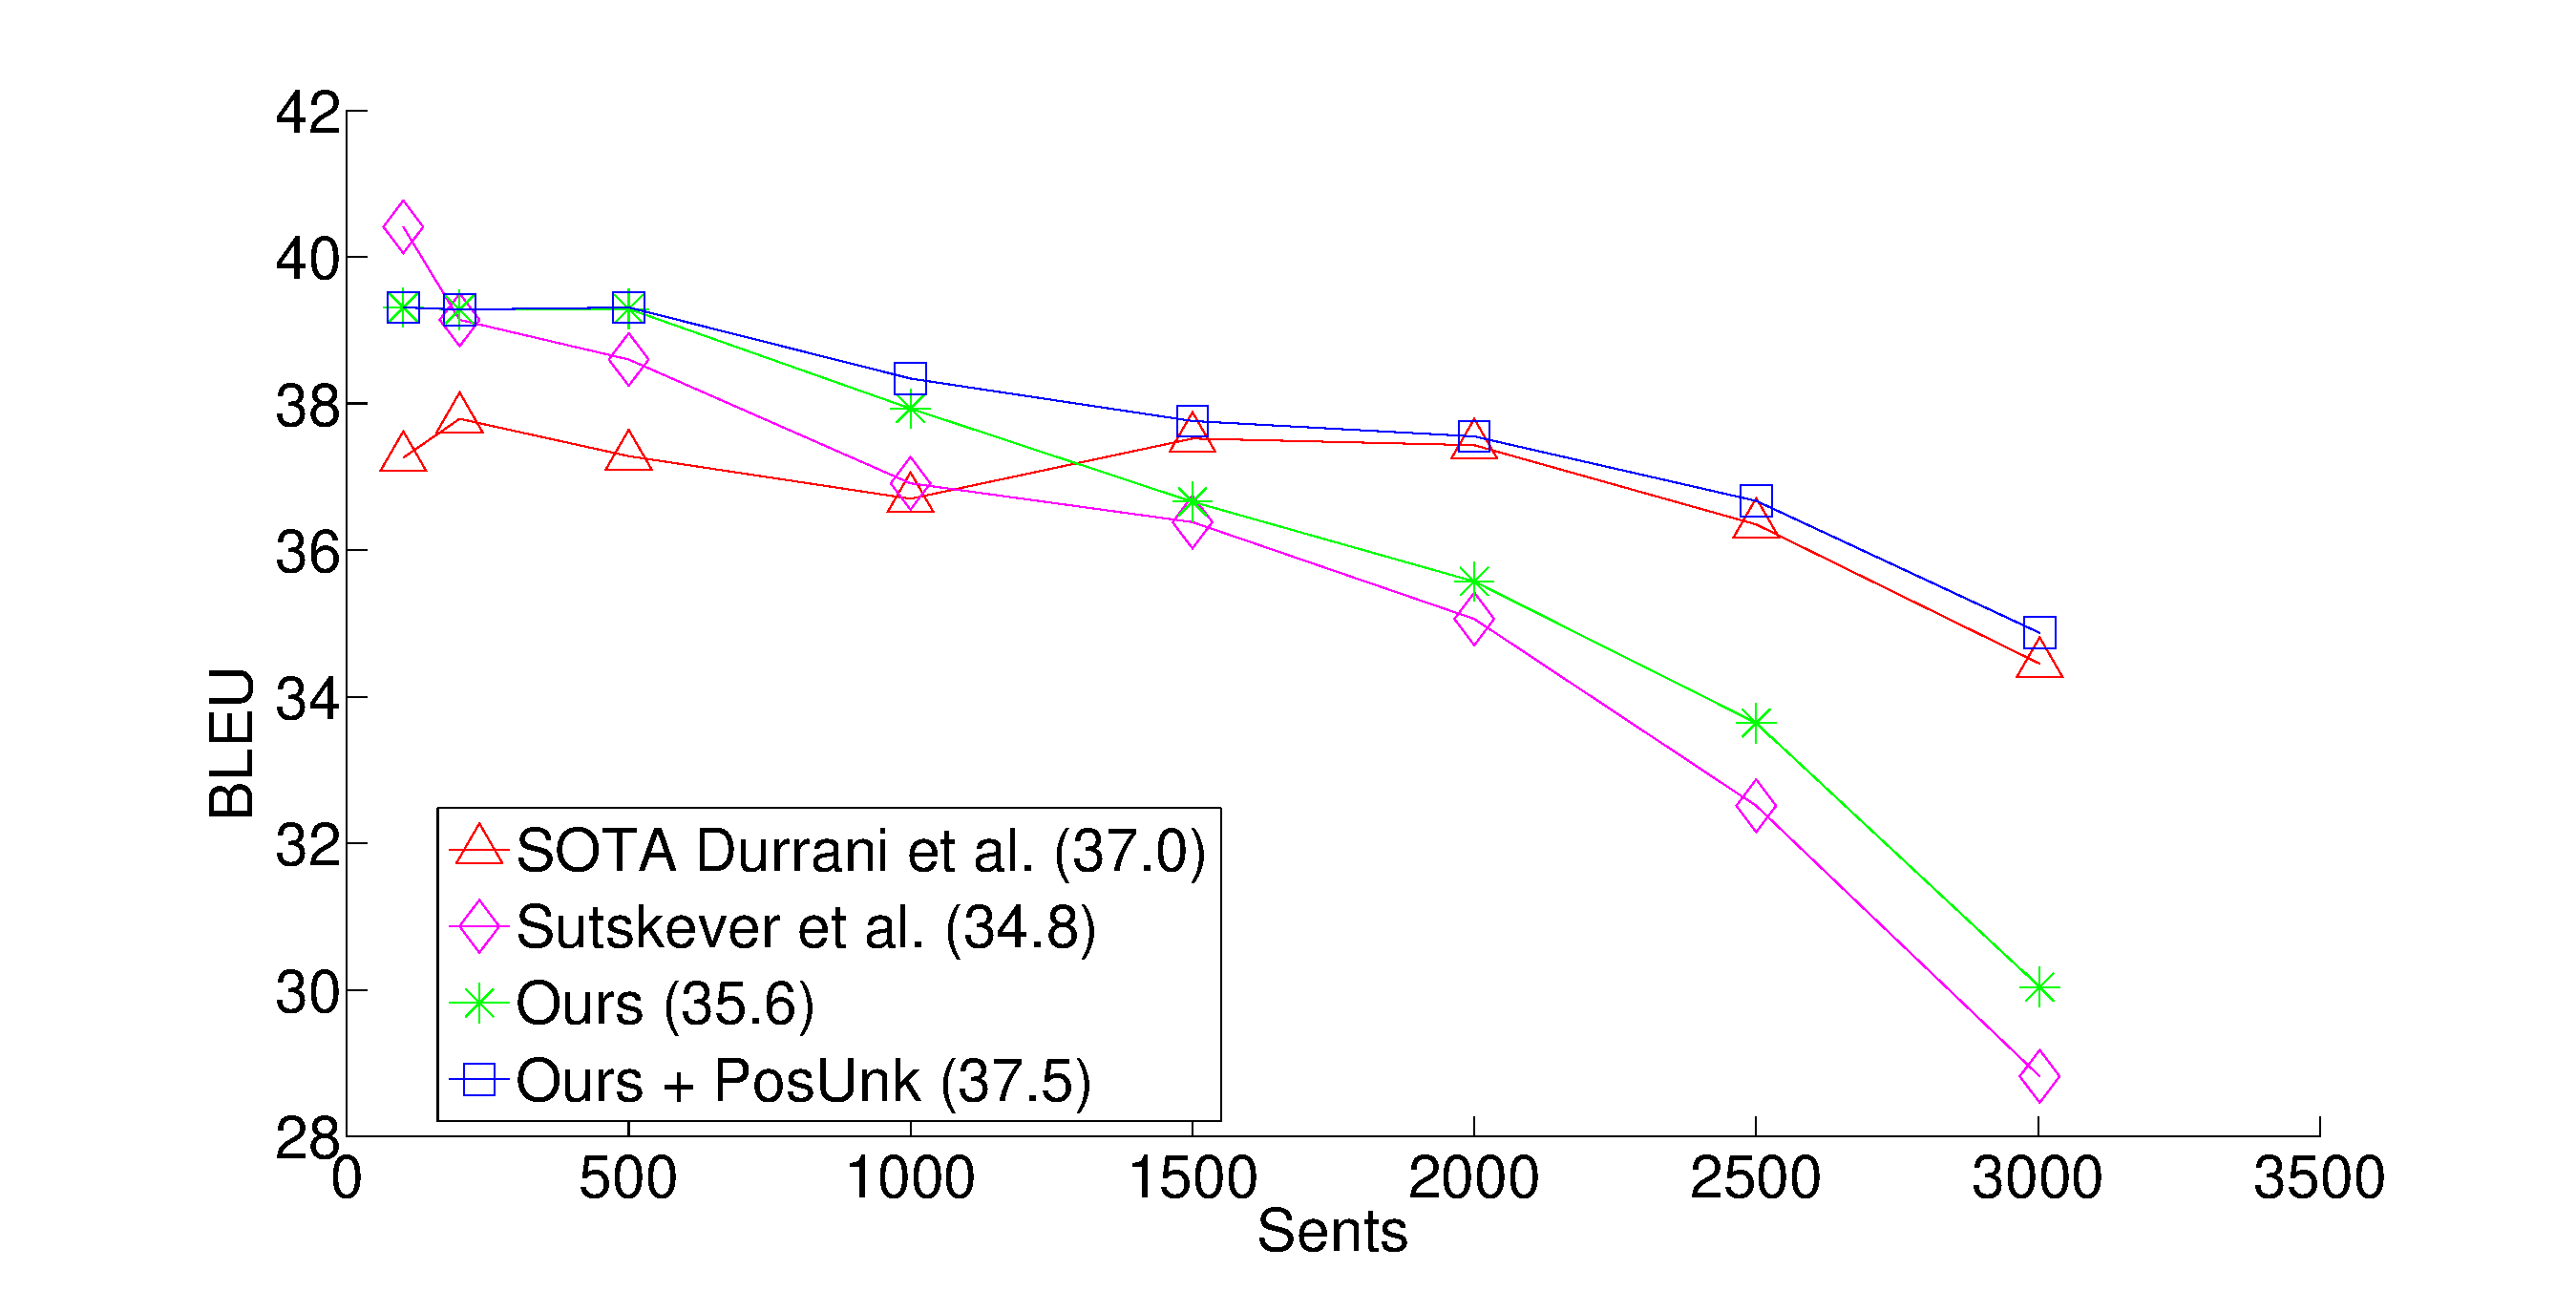
\includegraphics[width=0.7\textwidth, clip=true, trim= 95 0 230 0]{img/3-rare} % , angle=-90
\caption[Rare word translation]{{\bf Rare word translation} -- 
On the x-axis, I order newstest2014 sentences by their {\it average frequency rank} and divide the sentences into groups 
of sentences with a comparable prevalence of rare words. 
I compute the BLEU score of each group independently.} 
\label{f:rare}
\end{figure}


\subsection{Rare Word Models}
\label{subsec:rare_model_compare}

I examine the effect of the different rare word models presented in
Section~\ref{sec:rare}, namely: (a) {\it Copyable} -- which aligns the unknown
words on both the input and the target side by learning to copy indices, (b) the Positional All
({\it PosAll}) -- which predicts the aligned source positions for every target
word, and (c) the Positional Unknown ({\it PosUnk}) -- which predicts the aligned
source positions for only the unknown target words.\footnote{In this section and in section~\ref{subsec:effects},
all models are trained on the unreversed sentences, and I use the following hyperparameters: 
I initialize the parameters uniformly in [-0.1, 0.1], the learning rate is 1, the maximal gradient norm is 1, 
with a source vocabulary of 90k words, and a target vocabulary of 40k (see Section~\ref{subsec:train_details} for more details).
While these LSTMs do not achieve the best possible performance, it is still useful to analyze them.}
It is also interesting to measure the improvement obtained when no alignment information is used during training.
As such, I include a baseline model with no alignment knowledge ({\it NoAlign}) in which I simply assume that the $i^{\textrm{th}}$ unknown word on the target
sentence is aligned to the $i^{\textrm{th}}$ unknown word in the source sentence.

\begin{figure}
\centering
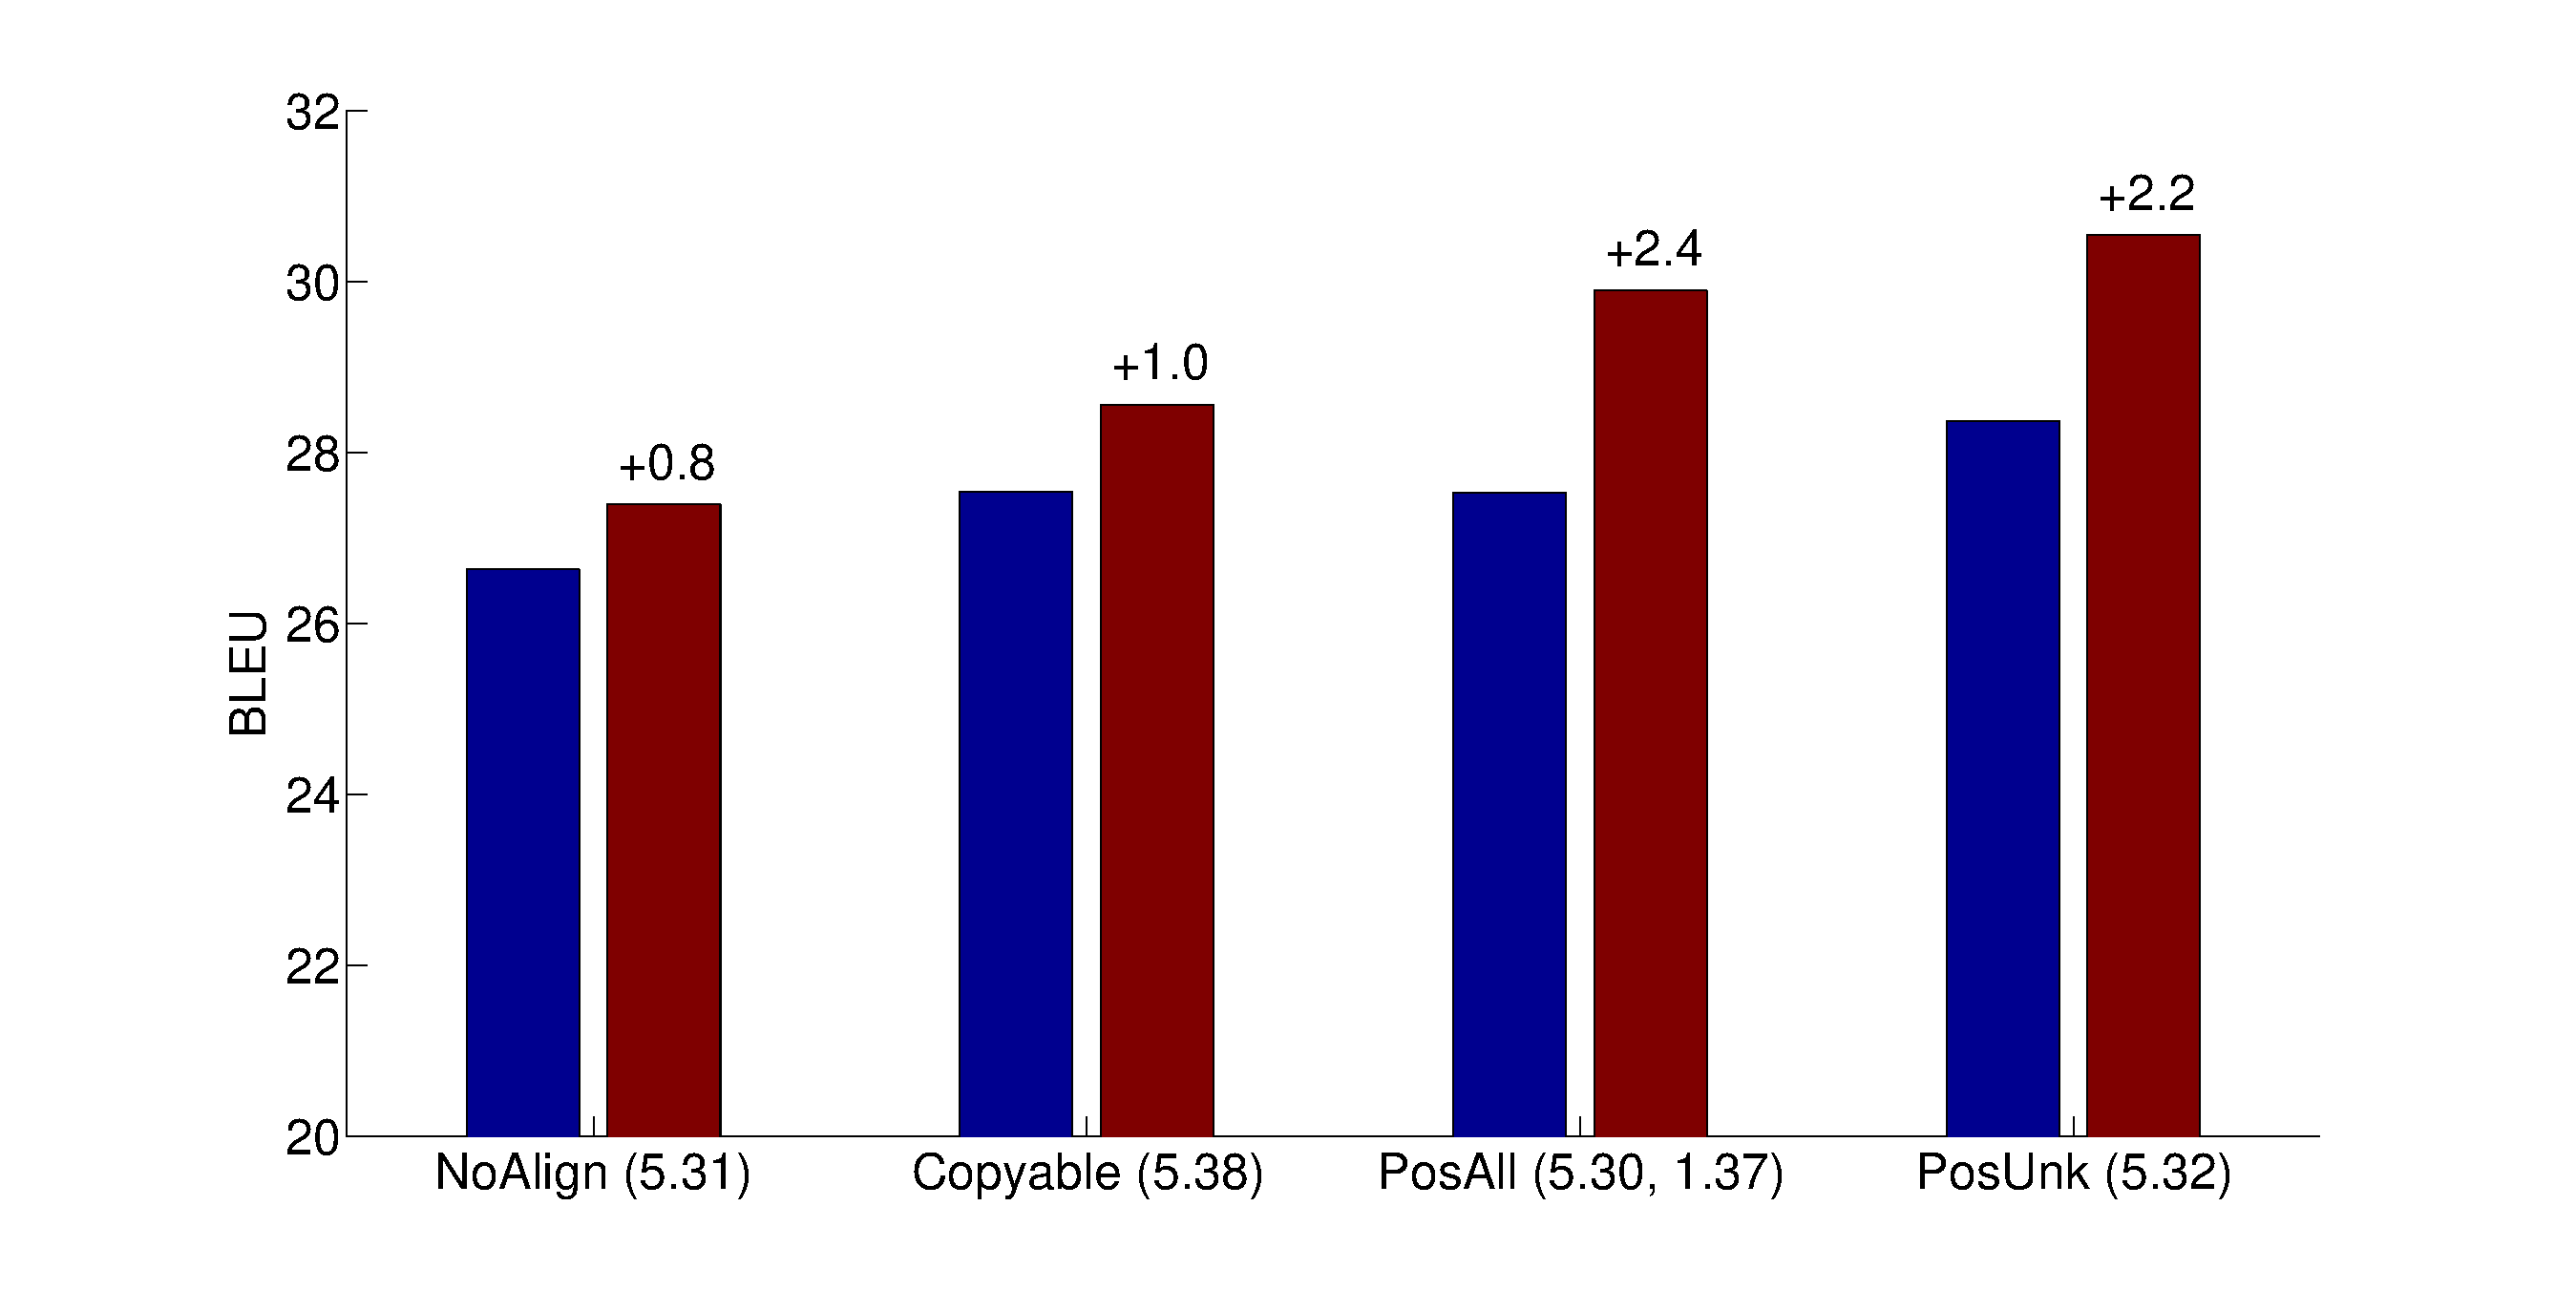
\includegraphics[width=0.7\textwidth, clip=true, trim= 105 0 140 0]{img/3-compare} % , angle=-90
\caption[Rare word models]{{\bf Rare word models} -- 
translation performance of 6-layer LSTMs:
a model that uses no alignment ({\it NoAlign}) 
and the other rare word models ({\it Copyable, PosAll, PosUnk}). 
For each model, I show results before ({\it left}) and after ({\it right}) the rare word translation as well as the perplexity (in parentheses).
For {\it PosAll}, I report the perplexities of predicting the words and the positions.} 
\label{f:compare}
\end{figure}

 
From the results in Figure~\ref{f:compare}, a simple monotone
alignment assumption for the {\it NoAlign} model yields a modest gain of
0.8 BLEU points. If I train the model to predict the alignment, then the {\it Copyable} model
offers a slightly better gain of 1.0 BLEU. Note, however, that English
and French have similar word order structure, so it would be
interesting to experiment with other language pairs, such as English and
Chinese, in which the word order is not as monotonic. These harder language pairs 
potentially imply a smaller gain for the NoAlign model and a larger
gain for the Copyable model. 
I leave it for future work.

The positional models ({\it PosAll} and {\it PosUnk}) 
improve translation performance by more than 2 BLEU points. 
This proves that the limitation of the copyable model, which forces
it to align each unknown output word with an unknown input word, is considerable.  
In contrast, the positional models can align the unknown target words with any source word,
and as a result, post-processing has a much stronger effect. 
The PosUnk model achieves better translation results than
the PosAll model which suggests that it is easier to train the LSTM on shorter sequences. 

\subsection{Other Effects}
\label{subsec:effects}
{\bf Deep LSTM architecture} --  I compare PosUnk models trained with different number of layers (3, 4, and 6). 
I observe that the gain obtained by the PosUnk model increases in tandem with the overall accuracy of the model, which is consistent 
with the idea that larger models can point to the appropriate source word more accurately.
Additionally, I observe that on average, each extra LSTM layer provides roughly 1.0 BLEU point improvement as demonstrated in Figure~\ref{f:depth}. 

\begin{figure}[tbh!]
\centering
\includegraphics[width=0.7\textwidth, clip=true, trim= 0 0 0 0]{img/3-depth} % , angle=-90
\caption[Effect of depths]{{\bf Effect of depths} -- BLEU scores achieved by {\it PosUnk} models of various depths (3, 4, and 6) before and after the rare word translation. 
 Notice that the PosUnk model is more useful on more accurate models. }
\label{f:depth}
\end{figure}

{\bf Perplexity and BLEU} -- Lastly, I find it interesting to observe a strong correlation 
between the perplexity (my training objective) and the translation quality as measured by BLEU. 
Figure~\ref{f:cor} shows the performance of a 4-layer LSTM, in which I compute both perplexity and 
BLEU scores at different points during training. I find that on average, a reduction of 0.5 perplexity 
gives us roughly 1.0 BLEU point improvement.
\begin{figure}[tbh!]
\centering
\includegraphics[width=0.7\textwidth, clip=true, trim= 0 0 0 0]{img/3-cor} % , angle=-90
\caption[Perplexity vs. BLEU]{{\bf Perplexity vs. BLEU} -- I show the correlation by evaluating an LSTM model with 4 layers at various stages of training. 
} 
\label{f:cor}
\end{figure}


\subsection{Sample Translations}
I present three sample translations of my best system
(with \bestbleuunk{} BLEU) in Table~\ref{t:sample}. In my  first example,
the model translates all the
unknown words correctly: {\it 2600}, {\it orthop{\'e}diques}, and {\it
cataracte}. It is interesting to observe that the model can accurately predict
an alignment of distances of 5 and 6 words. The second
example highlights the fact that my model can translate long
sentences reasonably well and that it was able to
correctly translate the unknown word for {\it JPMorgan} at the very far end of
the source sentence. Lastly, my examples also reveal several
penalties incurred by my model: (a) incorrect entries in the word dictionary, as with {\it n\'{e}gociateur} vs. {\it trader} in the second example, 
%identical meaning with different words, as with {\it n\'{e}gociateur} vs. {\it trader} in the second example, 
and (b) incorrect alignment prediction, such as when 
 \unkpostext{3} is incorrectly aligned
with the source word {\it was} and not with {\it abandoning}, which resulted in an
incorrect translation in the third sentence.

\begin{table*}[tbh!]
\centering
\resizebox{13.5cm}{!}{
\begin{tabular}{c|p{12cm}}
\bf{} & \bf{Sentences}\\
  \hline
src & An additional {\it 2600} operations including {\it orthopedic} and {\it cataract} surgery will help clear a backlog .\\
  \hline
trans & En outre , \unkpos{1} op{\'e}rations suppl{\'e}mentaires , dont la chirurgie \unkpos{5} et la \unkpos{6} , permettront de r{\'e}sorber l' arri{\'e}r{\'e} .\\
  \hline
+unk & En outre , {\it 2600} op{\'e}rations suppl{\'e}mentaires , dont la chirurgie {\it orthop{\'e}diques} et la {\it cataracte} , permettront de r{\'e}sorber l' arri{\'e}r{\'e} .\\
  \hline
tgt & 2600 op{\'e}rations suppl{\'e}mentaires , notamment dans le domaine de la chirurgie orthop{\'e}dique et de la cataracte , aideront {\`a} rattraper le retard .\\
  \hline
  \hline
src & This {\it trader} , Richard {\it Usher} , left RBS in {\it 2010} and is understand to have be given leave from his current position as European head of forex spot trading at {\it JPMorgan} .\\
  \hline
trans & Ce \unkpos{0} , Richard \unkpos{0} , a quitt{\'e} \unkpos{1} en 2010 et a compris qu' il est autoris{\'e} {\`a} quitter son poste actuel en tant que leader europ{\'e}en du march{\'e} des points de vente au \unkpos{5} .\\
  \hline
+unk & Ce {\it n\'{e}gociateur} , Richard {\it Usher} , a quitt{\'e} RBS en {\it 2010} et a compris qu' il est autoris{\'e} {\`a} quitter son poste actuel en tant que leader europ{\'e}en du march{\'e} des points de vente au {\it JPMorgan} .\\
  \hline
tgt & Ce trader , Richard Usher , a quitt{\'e} RBS en 2010 et aurait {\'e}t{\'e} mis suspendu de son poste de responsable europ{\'e}en du trading au comptant pour les devises chez JPMorgan \\
  \hline
  \hline
src & But concerns have grown after Mr {\it Mazanga} was quoted as saying {\it Renamo} {\it was} abandoning the 1992 peace accord .\\
  \hline
trans & Mais les inqui{\'e}tudes se sont accrues apr{\`e}s que M. \unkpos{3} a d{\'e}clar{\'e} que la \unkpos{3} \unkpos{3} l' accord de paix de 1992 .\\
  \hline
+unk & Mais les inqui{\'e}tudes se sont accrues apr{\`e}s que M. {\it Mazanga} a d{\'e}clar{\'e} que la {\it Renamo} {\it {\'e}tait} l' accord de paix de 1992 .\\
  \hline
tgt & Mais l' inqui{\'e}tude a grandi apr{\`e}s que M. Mazanga a d{\'e}clar{\'e} que la Renamo abandonnait l' accord de paix de 1992 .\\
\end{tabular}
}
\caption[Sample translations]{{\bf Sample translations} -- the table shows the source ({\it src}) and the translations of my best model before ({\it trans}) and after ({\it +unk}) unknown word translations. I also show the human translations ({\it tgt}) and italicize words that are involved in the unknown word translation process.}
\label{t:sample}
\end{table*}




\section{Conclusion}
\label{sec:conclude}
I have shown that a simple alignment-based technique can mitigate and even
overcome one of the main weaknesses of current NMT systems, which is
their inability to translate words that are not in their vocabulary.  
A key advantage of my technique is the fact that it is applicable to any NMT system and not
only to the deep LSTM model of \newcite{sutskever14}. At the time of this work, in 2014-2015, a technique
like mine is likely necessary if an NMT system is to achieve state-of-the-art performance
on machine translation.

I have demonstrated empirically that on the WMT'14 English-French translation task, my technique yields a 
consistent and substantial improvement of up to \bestunkimp{} BLEU points over various NMT systems of different architectures. 
Most importantly, with \bestbleuunk{} BLEU points, I have established the first NMT system that outperformed 
the best MT system on a WMT'14 contest dataset.

I will now switch gear to address a different problem in NMT,
that is the difficulty in translating long sentences. However, I will return back
to the topic of rare and unknown words in Chapter 5 to present an even better treatment to that problem.






\chapter{Attention Mechanisms}
\label{c:attention}
While I have demonstrated in the previous chapter that Neural Machine Translation (NMT) can achieve state-of-the-art performance in
large-scale translation tasks such as from English to French, it is still challenging for NMT to handle long sentences as observed by \newcite{bog15}.
One effective way to address such problem is through the attention mechanism, which has gained popularity recently in
training neural networks, allowing models to learn alignments between different
modalities, e.g., between image objects and agent actions in the dynamic control
problem \cite{mnih14}, between speech frames and text in the speech recognition
task \cite{jan14},  or between visual features of a picture and its text
description in the image caption generation task \cite{xu15}. In the context of
NMT, \newcite{bog15} has successfully applied such attentional mechanism to
jointly translate and align words. To the best of my knowledge during the time of this work, there has not
been any other work exploring the use of attention-based architectures for NMT.

\begin{figure}
\centering
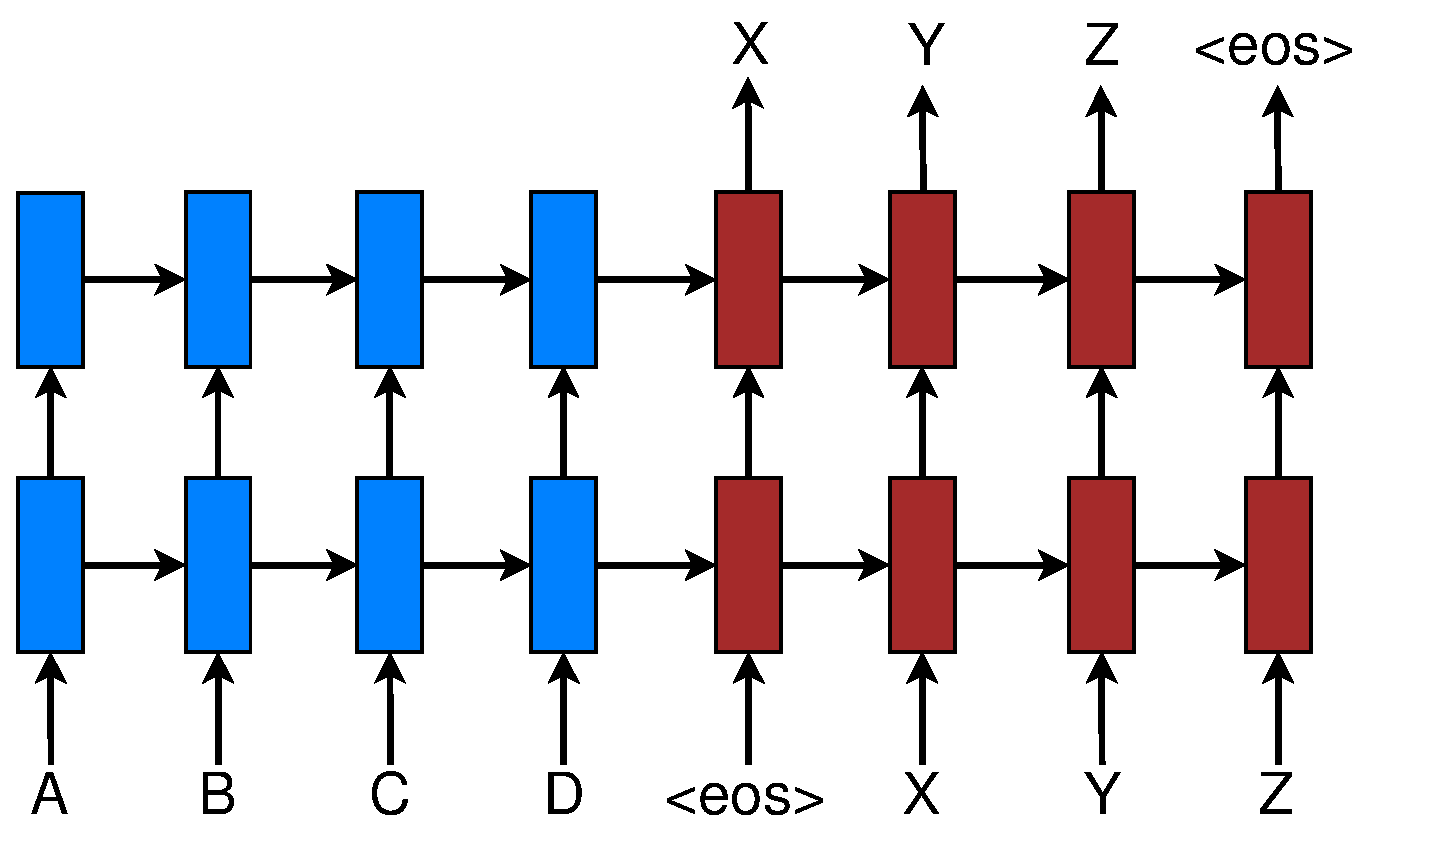
\includegraphics[width=0.45\textwidth, clip=true, trim= 0 0 0 0]{img/4-lstm} % , angle=-90
\caption[Neural machine translation]{{\bf Neural machine translation} -- a stacking recurrent architecture for translating a source sequence \texttt{A B C D} into a target sequence \texttt{X Y Z}. Here, \eos{} marks the end of a sentence.
} 
\label{f:lstm}
\end{figure}

In this work, I design, with simplicity and effectiveness in mind, two novel
types of attention-based models: a {\it global} approach in which all source
words are attended and a {\it local} one whereby only a subset of source words
are considered at a time. The former approach resembles the model of
\cite{bog15} but is simpler architecturally. The latter can be viewed as an
interesting blend between the {\it hard} and {\it soft} attention models
proposed in \cite{xu15}: it is computationally less expensive than the
global model or the soft attention; at the same time, unlike the hard attention,
the local attention is
differentiable almost everywhere, making it easier to implement and
train.\footnote{There is a recent work by \newcite{draw15}, which is very
similar to my local attention and applied to the image generation task.
However, as I detail later, my model is much simpler and can achieve good performance for NMT.} Besides, I also examine various
alignment functions for my attention-based models.

Following \cite{sutskever14,luong15}, I use the stacking LSTM architecture for our NMT systems, as illustrated in Figure~\ref{f:lstm}, together with the LSTM unit defined in \cite{zaremba14}.
The experimental results demonstrate that both of my approaches are
effective in the WMT translation tasks between English and German in  both
directions. My attentional models yield a boost of up to \attngain{} BLEU over
non-attentional systems which already incorporate known techniques such as
dropout. For English to German translation, I achieve new state-of-the-art
(SOTA)
results for both WMT'14 and WMT'15, outperforming previous SOTA systems, backed by
NMT models and $n$-gram LM rerankers, by more than 1.0 BLEU. I conduct
extensive analysis to evaluate my models in terms of learning, the ability to
handle long sentences, choices of attentional architectures, alignment quality, and translation
outputs. 

\section{Attention-based Models}
\label{sec:attn}
Unlike the basic NMT systems \cite{kal13,sutskever14,cho14,luong15}, in which the source representation is only used once to initialize the decoder hidden state, the idea of the {\it attention mechanism} explored in \cite{bog15,jean15} and this work is to provide a ``random access memory'' of source hidden states which one can constantly refer to as translation progresses.
The various attention-based models proposed in this work can be classified into two broad categories, {\it global} and {\it local}. These classes differ in terms of whether the ``attention'' is placed on all source positions or on only a few source positions. I illustrate these two model types in Figure~\ref{f:soft_attn} and \ref{f:hard_attn} respectively.

Common to these two types of models is the fact that at each time step $t$ in the decoding phase, both approaches first take as input the hidden state $\hi$ at the top layer of a stacking LSTM. The goal is then to derive a context vector $\co$ that captures relevant source-side information to help predict the current target word $\tgt{t}$. While these models differ in how the context vector $\co$ is derived, they share the same subsequent steps. 
Specifically, given the target hidden state $\hi$ and the source-side context vector $\co$, I employ a simple concatenation layer to combine the information from both vectors to produce an attentional hidden state as follows:
\begin{equation}
\hs = \tanh(\W{c}[\co; \hi])
\label{e:hs}
\end{equation} 

The attentional vector $\hs$ is then fed through the softmax layer to produce the predictive distribution formulated as:
\begin{equation}
p(\tgt{t}|\tgt{<t},\src{}) = \softmax(\W{s}\hs)
\label{e:predict}
\end{equation} 

I now detail how each model type computes the source-side context vector $\co$.

\subsection{Global Attention}
\label{subsec:global}
\begin{figure}
\centering
%\psgrid
\rput(7.1,6.6){$\tgt{t}$}
\rput(2.7,4){$\co$}
\rput(5,3.1){$\al$}
\rput(7.9,1.9){$\hi$}
\rput(7.9,6){$\hs$}
\rput(0.3,2.3){$\his$}
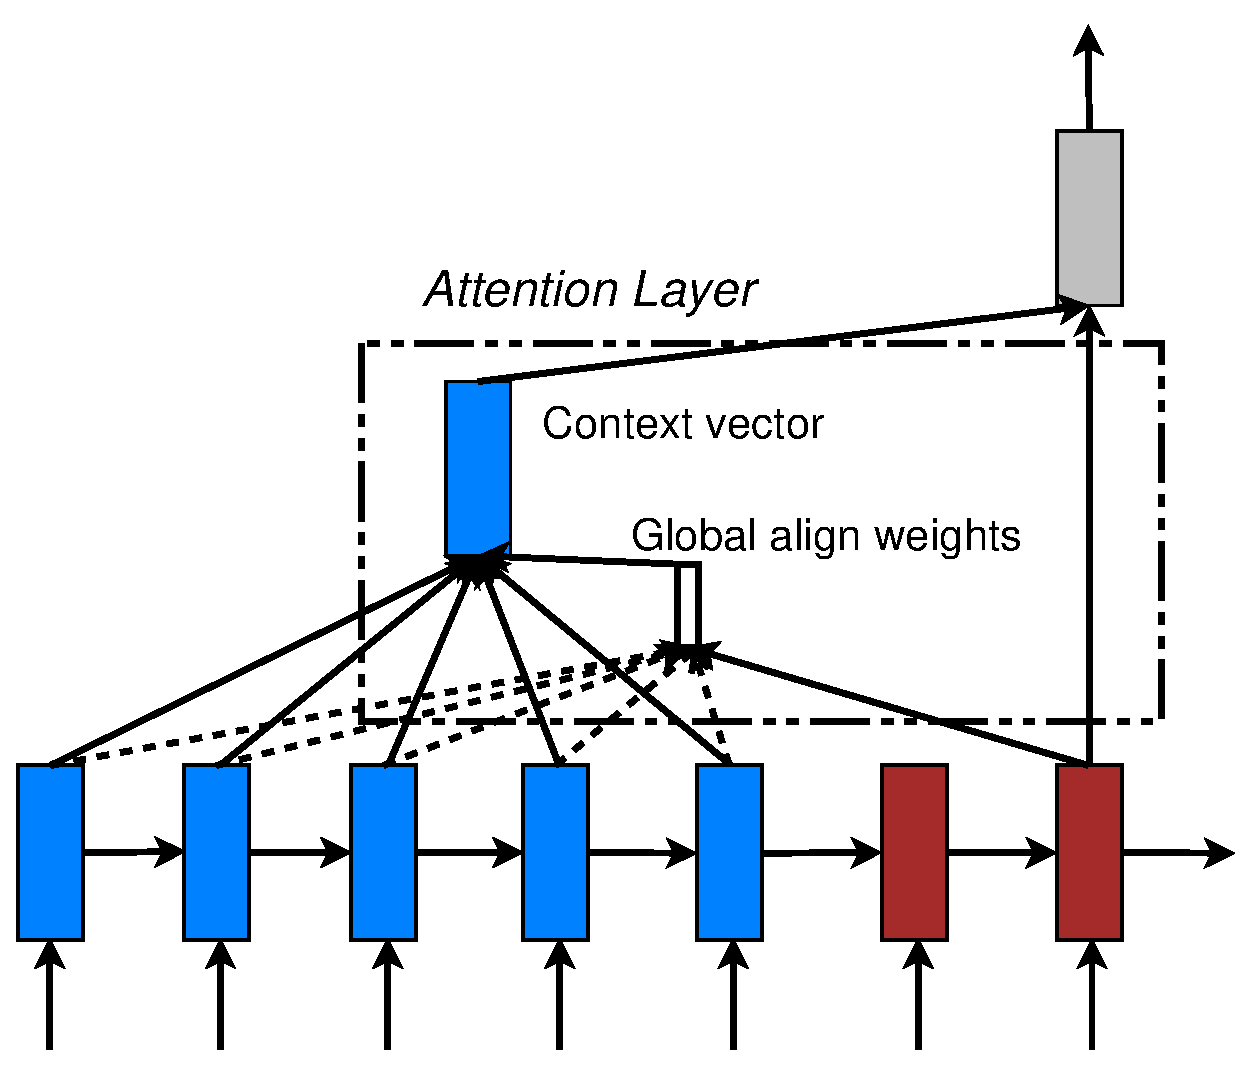
\includegraphics[width=0.55\textwidth, clip=true, trim= 0 0 0 0]{img/4-attn_soft} % , angle=-90
\caption[Global attentional model]{{\bf Global attentional model} -- at each time step $t$, the model infers a {\it variable-length} alignment weight vector $\al$ based on the current target state $\hi$ and all source states $\his$. A global context vector $\co$ is then computed as the weighted average, according to $\al$, over all the source states. 
} 
\label{f:soft_attn}
\end{figure}

The idea of a global attentional model is to consider all the hidden states of
the encoder when deriving the context vector $c_t$. In this model type, a
variable-length alignment vector $\al$, whose size equals the number of time
steps on the source side, is derived by comparing the current target hidden
state $\hi$ with each source hidden state $\his$:
\begin{align}
\label{e:al}
\al(s)&=\alignf(\hi, \his) \\
&=\frac{\exp \open{\score(\hi, \his)}}{\sum_{s'} \exp \open{\score(\hi,
\MB{\bar{h}}_{s'})}} \notag
\end{align}
Here, $\score$ is referred to as a {\it content-based} function for which I consider three different
alternatives:
\begin{equation*}
\score(\hi, \his)\!=\!\begin{cases}
    \tp{\hi} \his & \mbox{{\it dot}}\\
    \tp{\hi} \MB{W_a} \his & \mbox{{\it general}} \\
    \tp{\MB{v}_a}\tanh\open{\MB{W_a} [\hi; \his]} & \mbox{{\it concat}}
\end{cases}
\end{equation*}

In addition, in our early attempts to build attention-based models, I used
a {\it location-based} function in which the alignment scores are
computed from solely the target hidden state $\hi$ as
follows:
\begin{equation}
\al = \softmax(\W{a}\hi) \mbox{ } \mbox{ } \mbox{ } \mbox{ } \mbox{ } \mbox{ } \mbox{ } \mbox{ } \mbox{ } \mbox{ } \mbox{ } \mbox{ } \mbox{ } \mbox{ } \mbox{ } \mbox{ } \mbox{{\it location}}
\label{e:location}
\end{equation}
Given the alignment vector as weights, the
context vector $c_t$ is computed as the  weighted average over all the source hidden states.\footnote{\eq{e:location} implies that
all alignment vectors $\al$ are of the same length. For short sentences, I only
use the top part of $\al$ and for long sentences, I ignore words near the end.}

\textit{Comparison to \cite{bog15}} --
% An example of such model is the work of \newcite{bog15}. 
While our global attention approach is similar in spirit to the model proposed
by \newcite{bog15}, there are several key differences which reflect how I have
both simplified and generalized from the original model. First, I simply use
hidden states at the top LSTM layers in both the encoder and decoder as
illustrated in Figure~\ref{f:soft_attn}. \newcite{bog15}, on the other hand,
use the concatenation of the forward and backward source 
hidden states in the bi-directional encoder and target hidden
states in their non-stacking uni-directional decoder. Second, our computation
path is simpler; I go from $\hi \rightarrow \al \rightarrow \co \rightarrow
\hs$ then make a prediction as detailed in \eq{e:hs}, \eq{e:predict}, and
Figure~\ref{f:soft_attn}. On the other hand, at any time $t$, \newcite{bog15} build from the previous hidden state $\hid{t-1} \rightarrow \al \rightarrow \co \rightarrow \hi$, which, in turn, goes through a deep-output and a maxout layer before making predictions.\footnote{I will refer to this difference again in Section~\ref{subsec:input}.} Lastly, \newcite{bog15} only experimented with one alignment function, the {\it concat} product; whereas I show later that the other alternatives are better.

\subsection{Local Attention}
\begin{figure}
\centering
%\psgrid
\rput(7.1,6.6){$\tgt{t}$}
\rput(2.7,4){$\co$}
\rput(3.8,2.9){$\al$}
\rput(7.9,1.9){$\hi$}
\rput(7.9,6){$\hs$}
\rput(6.5,3.4){$p_t$}
\rput(0.3,2.3){$\his$}
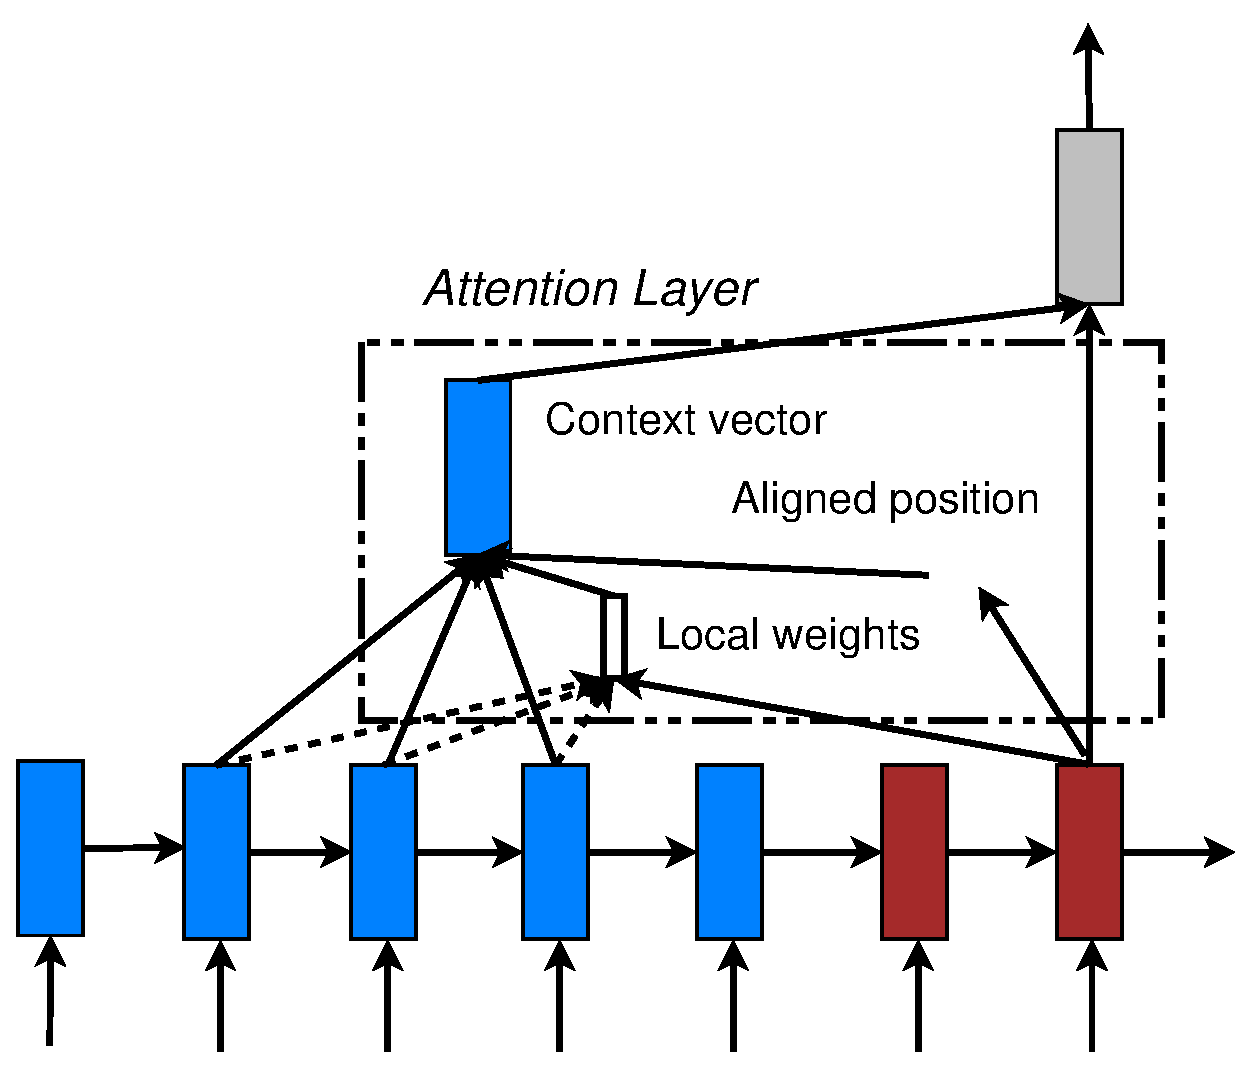
\includegraphics[width=0.55\textwidth, clip=true, trim= 0 0 0 0]{img/4-attn_hard} % , angle=-90
\caption[Local attention model]{{\bf Local attention model} -- the model first predicts a single
aligned position $p_t$ for the current target word. A window centered around the
source position $p_t$ is then used to compute a context vector $\co$, a weighted
average of the source hidden states in the window. The weights $\MB{\al}$ are
inferred from the current target state $\hi$ and those source states $\his$ in
the window.
%similar to the global attention model in Figure~\ref{f:soft_attn}, instead of producing a global alignment vector, 
} 
\label{f:hard_attn}
\end{figure}

The global attention has a drawback that it has to attend to all words on the
source side for each target word, which is expensive and can potentially render it impractical to
translate longer sequences, e.g., paragraphs or documents.
To address this deficiency, I propose a {\it local} attentional mechanism that
chooses to focus only on a small subset of the source positions per target word.

This model takes inspiration from the tradeoff between the {\it soft} and {\it
hard} attentional models proposed by \newcite{xu15} to tackle the image caption
generation task. In their work, soft attention refers to the global attention
approach in which weights are placed ``softly'' over all patches in the source
image. The hard attention, on the other hand, selects one patch
of the image to attend to at a time. While less expensive at inference time, the
hard attention model is non-differentiable and requires more complicated
techniques such as variance reduction or reinforcement learning to train.

My local attention mechanism selectively focuses on a small window of
context and is differentiable. This approach has an advantage of avoiding the expensive computation incurred in
the soft attention and at the same time, is easier to train than the hard
attention approach.
In concrete details, the model first generates an aligned position $p_t$ for each target word at time $t$. The
context vector $\co$ is then derived as a weighted average over the set of source hidden states within the window $[p_t-D, p_t+D]$; $D$ is
empirically selected.\footnote{If the window crosses the sentence boundaries, I
simply ignore the outside part and consider words in the window.} Unlike the global approach, the local alignment vector $\al$ is now fixed-dimensional, i.e., $\inR{2D+1}$. %is generated in the same manner as the global attentional model except that its dimension is $(2D+1)$.
I consider two variants of the model as below.

\textit{Monotonic} alignment ({\bf \localm{}}) -- I simply set % 
$\pt\!=\!t$ assuming that source and target sequences are roughly
monotonically aligned. The alignment vector $\al$ is defined according to
\eq{e:al}.\footnote{{\it local-m} is the same as
the global model except that the vector $\al$ is
fixed-length and shorter.} % This model is differentiable.

\textit{Predictive} alignment ({\bf \localp{}}) --  %
instead of assuming monotonic alignments, our model predicts an aligned position as follows:
\begin{equation}
\pt = S \cdot \sigmoid(\tp{\MB{v}_p}\tanh(\W{p}\hi)),
\label{e:p}
\end{equation}
$\W{p}$ and $\MB{v}_p$ are the model parameters which will be learned
to predict positions. $S$ is the source sentence length. As a result of $\sigmoid$, $\pt
\in [0, S]$. To favor alignment points near $\pt$, I place a Gaussian distribution centered around $\pt$ . Specifically, our alignment weights are now
defined as:
\begin{equation}
\al(s) = \alignf(\hi, \his) \exp \open{-\frac{(s-\pt)^2}{2\sigma^2}} 
\label{e:align_p}
\end{equation}
I use the same $\alignf$ function as in
\eq{e:al} and the standard deviation is empirically set as
$\sigma\!=\!\frac{D}{2}$. Note that $\pt$ is a {\it real} number; whereas $s$
is an {\it integer} within the window centered at $\pt$.\footnote{{\it local-p} is similar to the
local-m model except that I dynamically
compute $\pt$ and use a truncated Gaussian distribution to modify the original alignment
weights $\alignf(\hi, \his)$ as shown in \eq{e:align_p}. By utilizing $\pt$
to derive $\al$, I can compute backprop gradients for $\W{p}$ and $\MB{v}_p$.
This model is differentiable almost everywhere.} 

\textit{Comparison to \cite{draw15}} --
they have proposed a {\it selective attention} mechanism, very
similar to our local attention, for the image generation task. Their approach 
allows the model to select an image patch of varying location and zoom. I,
instead, use the same ``zoom'' for all target positions, which greatly
simplifies the formulation and still achieves good
performance.

\subsection{Input-feeding Approach}
\label{subsec:input}
In our proposed global and local approaches, the attentional decisions are made
independently, which is suboptimal. Whereas, in standard MT, a {\it coverage}
set is often maintained during the translation process to keep track of which
source words have been translated. Likewise, in attentional NMTs, alignment
decisions should be made jointly taking into account past alignment information.
To address that, I propose an {\it input-feeding} approach in which attentional
vectors $\hs$ are concatenated with inputs at the next time steps as illustrated in
Figure~\ref{f:input}.\footnote{If $n$ is the number of LSTM cells, the
input size of the first LSTM layer is $2n$; those of subsequent
layers are $n$.} The effects of having such connections are two-fold:
(a) I hope to make the model fully aware of previous alignment choices and (b)
I create a very deep network spanning both horizontally and vertically.

\begin{figure}
\centering
%\psgrid
\rput(3.5,6){$\hs$}
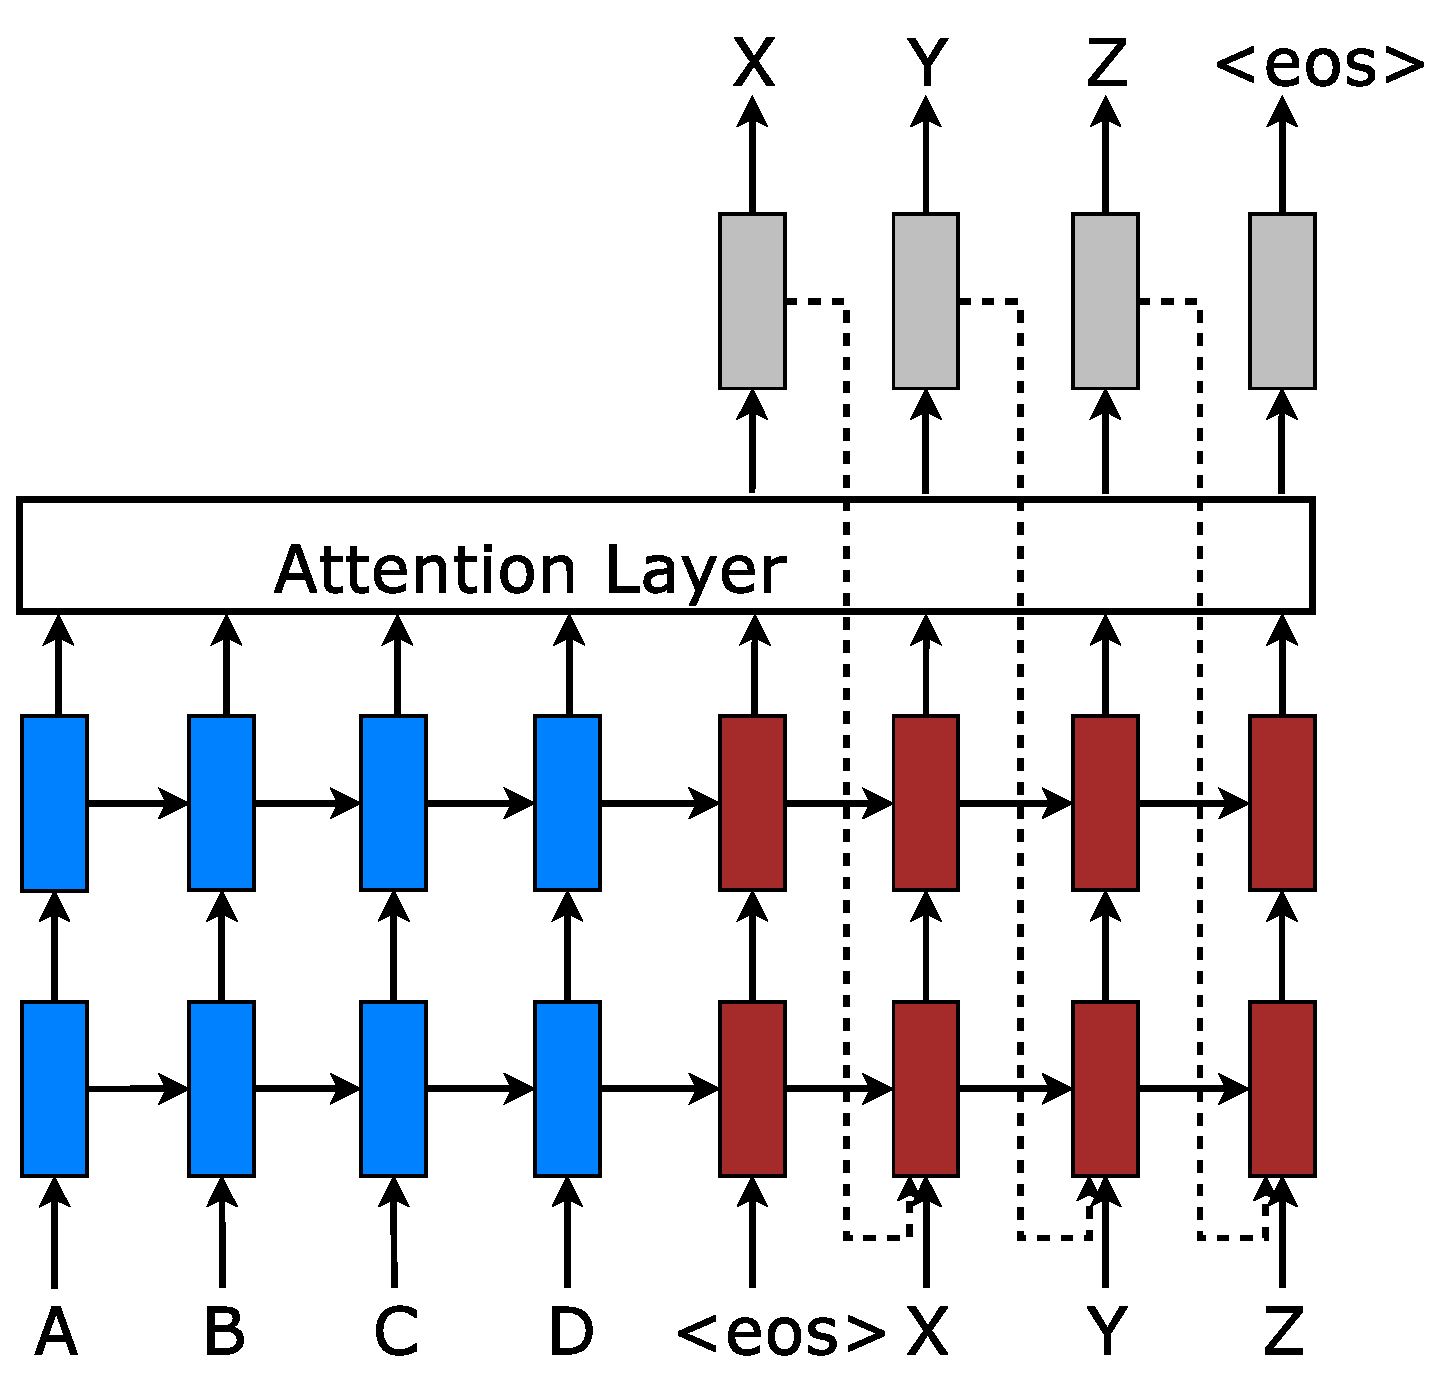
\includegraphics[width=0.5\textwidth, clip=true, trim= 0 0 0 0]{img/4-attn_input} % , angle=-90
\caption[Input-feeding approach]{{\bf Input-feeding approach} -- Attentional vectors $\hs$ are fed as inputs to the next time steps to inform the model about past alignment decisions.
} 
\label{f:input}
\end{figure}


{\it Comparison to other work} -- \newcite{bog15}
use context vectors, similar to
our $\co$, in building subsequent hidden states, which can also 
achieve the ``coverage'' effect. However, there has not been any analysis of 
whether such connections are useful as done in this work. Also,
our approach is more general; as illustrated in Figure~\ref{f:input}, it can be
applied to general stacking recurrent architectures, including non-attentional
models.

\newcite{xu15} propose a {\it doubly attentional} approach with an
additional constraint added to the training objective to make sure the model
pays equal attention to all parts of the image during the caption generation process. Such a constraint can also be useful to capture the coverage set effect in NMT that I mentioned earlier. However, I chose to use the input-feeding approach since it provides flexibility for the model to decide on any attentional constraints it deems suitable.

\section{Experiments}
\label{sec:exp}
I evaluate the effectiveness of my models on the WMT translation tasks between
English and German in both directions. newstest2013 (3000 sentences) is used as
a development set to select my hyperparameters. Translation performances are
reported in case-sensitive BLEU \cite{Papineni02bleu} on newstest2014 (2737 sentences) and
newstest2015 (2169 sentences). Following \cite{luong15}, I report
translation quality using two types of BLEU: (a) {\it
tokenized}\footnote{All texts are tokenized with \texttt{tokenizer.perl} and BLEU
scores are computed with \texttt{multi-bleu.perl}.} BLEU to be comparable with
existing NMT work and (b) {\it NIST}\footnote{With the \texttt{mteval-v13a}
script as per WMT guideline.} BLEU to be comparable
with WMT results.

\begin{table*}[tbh!]
\centering
\resizebox{15cm}{!}{
\begin{tabular}{l|r|c}
\bf{System} & \bf{Ppl} & \bf{BLEU}\\
  \hline
Winning WMT'14 system -- {\it phrase-based + large LM} \cite{buck14} &  & 20.7\\
  \hline
\multicolumn{3}{l}{{\it Existing NMT systems}}\\
  \hline
RNNsearch \cite{jean15} &  & 16.5\\
RNNsearch + unk replace \cite{jean15} &  & 19.0\\
RNNsearch + unk replace + large vocab + {\it ensemble} 8 models \cite{jean15} &  & {\bf 21.6}\\
  \hline
\multicolumn{3}{l}{{\it My NMT systems}}\\
  \hline
Base & 10.6 & 11.3\\
Base + reverse & 9.9 & 12.6 ({\it +1.3})\\
Base + reverse + dropout & 8.1 & 14.0 ({\it +1.4})\\
  \hdashline
Base + reverse + dropout + global attention ({\it location}) & 7.3 & 16.8 ({\it +2.8}) \\
Base + reverse + dropout + global attention ({\it location}) + feed input & 6.4
& 18.1 ({\it +1.3}) \\
  \hdashline
Base + reverse + dropout + local-p attention ({\it general}) + feed input
& \multirow{ 2}{*}{5.9} & 19.0 ({\it +0.9}) \\
Base + reverse + dropout + local-p attention ({\it general}) + feed input + unk replace
&  & 20.9 ({\it +1.9}) \\
  \hdashline
{\it Ensemble} 8 models + unk replace &  & {\bf 23.0 ({\it +2.1})} \\
\end{tabular}
}
\caption[WMT'14 English-German results]{{\bf WMT'14 English-German results} -- shown are
the perplexities (ppl) and the {\it tokenized} BLEU scores of various systems on newstest2014. I highlight the {\bf
best} system in bold and give {\it progressive} improvements in italic between
consecutive systems. {\it local-p} referes to the local attention with 
predictive alignments. I indicate for each attention model the
alignment score function used in parentheses. 
}
\label{t:ende}
\end{table*}


\subsection{Training Details}
All my models are trained on the WMT'14 training data consisting of 4.5M
sentences pairs (116M English words, 110M German words). Similar to \cite{jean15}, I limit my vocabularies to be the top 50K most frequent words for both languages. Words not in these shortlisted vocabularies are converted into a universal token \unk{}. 

When training my NMT systems, following \cite{bog15,jean15}, I filter out
sentence pairs whose lengths exceed 50 words and shuffle mini-batches as I
proceed. My stacking LSTM models have 4 layers, each with 1000 cells, and
1000-dimensional embeddings. I follow \cite{sutskever14,luong15} in training
NMT with similar settings: (a) my parameters are uniformly initialized in
$[-0.1, 0.1]$, (b) I train for 10 epochs using plain SGD, (c) a simple learning
rate schedule is employed -- I start with a learning rate of 1; after 5 epochs,
I begin to halve the learning rate every epoch, (d) my mini-batch size is 128,
and (e) the normalized gradient is rescaled whenever its norm exceeds 5.
Additionally, I also use dropout with probability $0.2$ for my LSTMs as suggested by
\cite{zaremba14}. For dropout models, I train for 12 epochs and start halving
the learning rate after 8 epochs. For local
attention models, I empirically set the window size $D=10$.

My code is implemented in MATLAB.
When running on a single GPU device Tesla K40, I achieve a speed of 1K {\it
target} words per second. It takes 7--10 days to completely train a model.

\subsection{English-German Results}
I compare my NMT systems in the English-German task with various other
systems. These include the winning system in WMT'14
\cite{buck14}, a phrase-based system whose language models were trained on a
huge monolingual text, the Common Crawl corpus. For end-to-end NMT systems, to the best of my knowledge, \cite{jean15} is the only work experimenting with this language pair and currently the SOTA system.
I only present results for some of my attention models and will later
analyze the rest in Section~\ref{sec:analysis}. 

\begin{sloppypar}
As shown in Table~\ref{t:ende}, I achieve progressive improvements when
(a) reversing the source sentence, +$1.3$ BLEU, as proposed in \cite{sutskever14}
and (b) using dropout, +$1.4$ BLEU. On top of that, (c) the global
attention approach gives a significant boost of +$2.8$ BLEU, making 
 my model slightly better than the base attentional system of
 \newcite{bog15} (row {\it RNNSearch}). When (d) using the {\it input-feeding}
approach, I seize another notable gain of +$1.3$ BLEU and outperform their
system. The local attention model with predictive alignments (row {\it \localp}) proves
to be even better, giving us a further improvement of +$0.9$ BLEU on top of the
global attention model. 
It is interesting to observe the trend previously reported in
\cite{luong15} that perplexity strongly correlates with translation quality.
In total, I achieve a significant gain of
\attngain{} BLEU points over the non-attentional baseline, which already includes
known techniques such as source reversing and dropout.
\end{sloppypar}

The unknown replacement technique proposed in \cite{luong15,jean15} yields another nice
gain of +$1.9$ BLEU, demonstrating that my attentional models
do learn useful alignments for unknown works. Finally, by ensembling 8 different
models of various settings, e.g., using different attention approaches, with
and without dropout etc., I was able to achieve a {\it new SOTA} result of
$\sotaold{}$
BLEU, outperforming the existing best system \cite{jean15} by +$1.4$ BLEU.

\begin{table}[tbh!]
\centering
%\resizebox{8cm}{!}{
\begin{tabular}{l|c}
\bf{System} & \bf{BLEU}\\
  \hline
Top -- {\it NMT + 5-gram rerank} (Montreal) & 24.9 \\
  \hline
My ensemble 8 models + unk replace & {\bf 25.9} \\
\end{tabular}
%}
\caption[WMT'15 English-German results]{{\bf WMT'15 English-German results} -- {\it NIST} BLEU scores of the
winning entry in WMT'15 and my best one on newstest2015.}
\label{t:wmt15ende}
\end{table}

{\it Latest results in WMT'15} -- despite the fact that my models were trained
on WMT'14 with slightly less data, I test them on newstest2015 to demonstrate
that they can generalize well to different test sets. As shown in Table~\ref{t:wmt15ende}, my best
system establishes a {\it new SOTA} performance of $\sotanew{}$ BLEU,
outperforming the existing best system backed by NMT and a 5-gram LM reranker
by +$1.0$
BLEU.

\subsection{German-English Results}
I carry out a similar set of experiments for the WMT'15 translation task from German
to English. 
While my systems have not yet matched the performance of the 
SOTA system, I nevertheless show the effectiveness of my
approaches with large and progressive gains in terms of BLEU as illustrated in
Table~\ref{t:deen}. 
The {\it attentional} mechanism gives us +$2.2$ BLEU gain and on top of that, I
obtain another boost of up to +$1.0$ BLEU from the {\it input-feeding} approach.
Using a better alignment function, the content-based {\it dot} product one,
together with {\it dropout} yields another gain of +$2.7$ BLEU. Lastly, when
applying the unknown word replacement technique, I seize an additional +$2.1$
BLEU, demonstrating the usefulness of attention in aligning rare words.
\begin{table}
\centering
%\resizebox{8cm}{!}{
\begin{tabular}{l|r|c}
\bf{System} & \bf{Ppl.} & \bf{BLEU}\\
  \hline
\multicolumn{3}{l}{{\it WMT'15 systems}}\\
  \hline
SOTA -- {\it phrase-based} (Edinburgh) &  & {\bf 29.2}\\ %\cite{freitag14}
NMT + 5-gram rerank (MILA) &  & 27.6\\ %\cite{freitag14}
  \hline
\multicolumn{3}{l}{{\it My NMT systems}}\\
  \hline
Base (reverse) & 14.3 & 16.9\\
  \hdashline
+ global ({\it location}) & 12.7 & 19.1 ({\it +2.2}) \\
+ global ({\it location}) + feed & 10.9 & 20.1 ({\it +1.0})\\
  \hdashline
+ global ({\it dot}) + drop + feed & \multirow{ 2}{*}{9.7} & 22.8 ({\it +2.7})\\
+ global ({\it dot}) + drop + feed + unk &  & 24.9 ({\it +2.1})\\
  %\hdashline
%{\it Ensemble} 4 models + unk &  & {\bf xx} ({\it +1.2})\\
\end{tabular}
%}
\caption[WMT'15 German-English results]{{\bf WMT'15 German-English results} -- 
performances of various systems (similar to 
Table~\ref{t:ende}). The {\it base} system already includes source reversing
on which I add {\it global} attention, {\it drop}out, input {\it feed}ing, and
{\it unk} replacement.}
\label{t:deen}
\end{table}

\section{Analysis}
\label{sec:analysis}
I conduct extensive analysis to better understand my models in terms
of learning, the ability to handle long sentences, 
choices of attentional architectures, and alignment quality. All results
reported here are on English-German newstest2014.

\subsection{Learning curves}
I compare models built on top of one another
as listed in Table~\ref{t:ende}. It is
pleasant to observe in Figure~\ref{f:learn} a clear separation between non-attentional and attentional
models. The input-feeding approach and the local attention
model also demonstrate their abilities in driving the test costs lower. The
non-attentional model with 
dropout (the blue + curve) learns slower than other non-dropout models, but
as time goes by, it becomes more robust in terms of minimizing test errors.
\begin{figure}
\centering
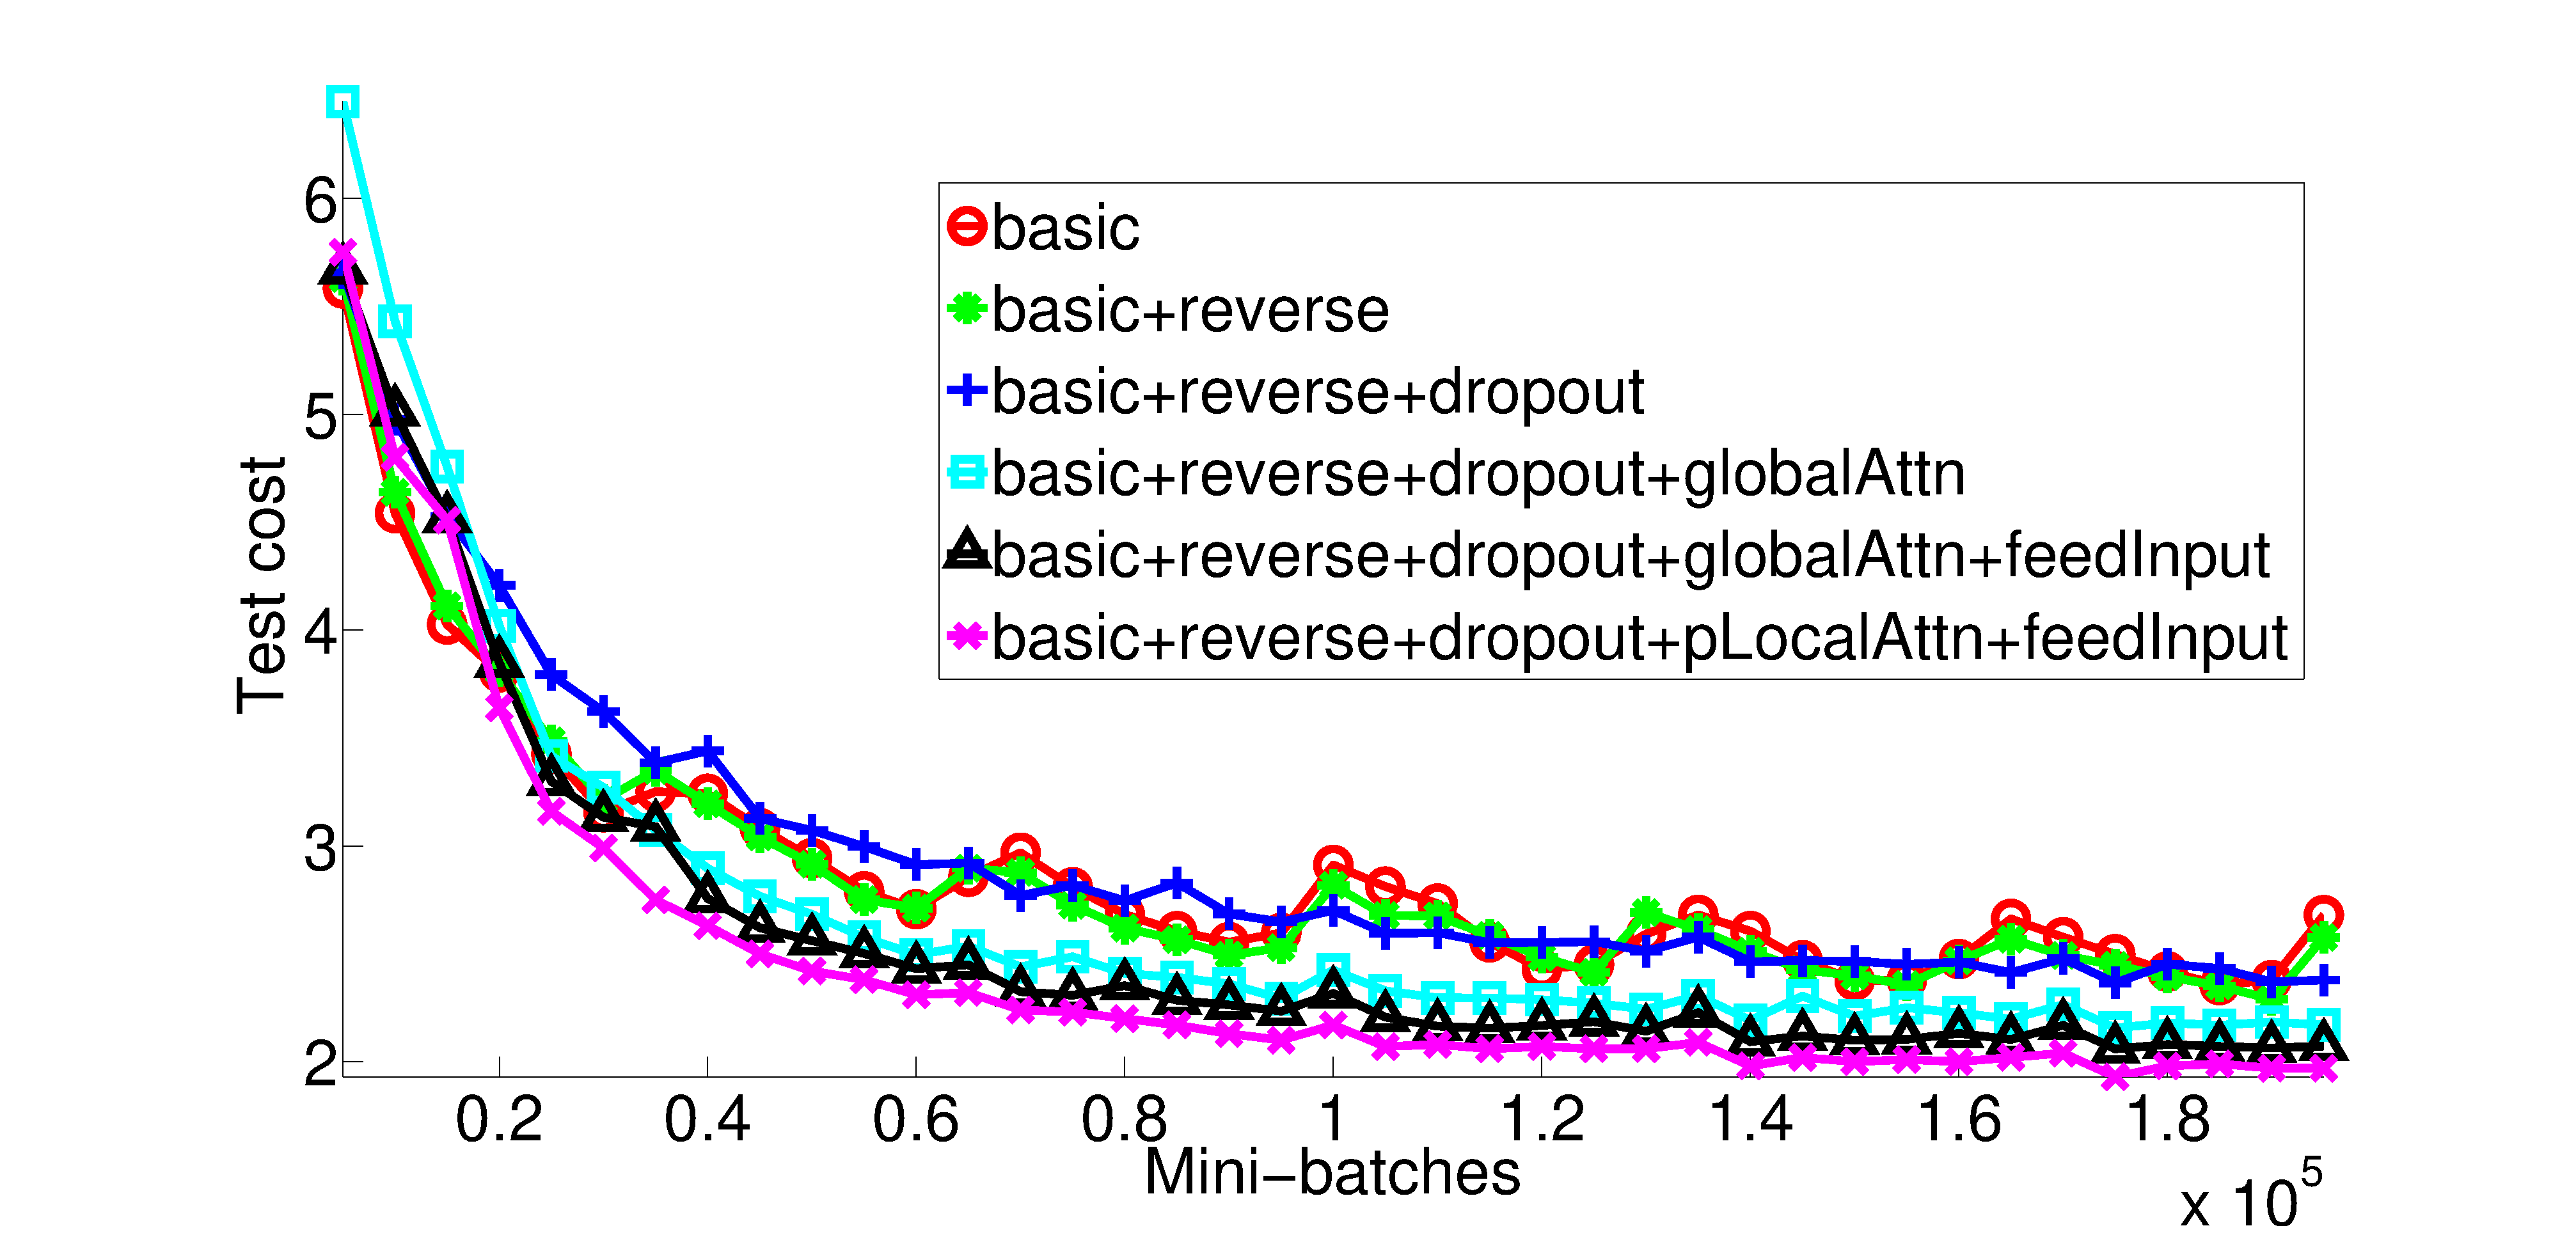
\includegraphics[width=0.7\textwidth, clip=true, trim=140 0 70 0]{img/4-learning} % , angle=-90
\caption[Learning curves]{{\bf Learning curves} -- test cost ($\ln$ perplexity) on newstest2014 for English-German NMTs as training progresses.
} 
\label{f:learn}
\end{figure}

\subsection{Effects of Translating Long Sentences}
I follow \cite{bog15} to group sentences of similar lengths together and
compute a BLEU score per group. Figure~\ref{f:length} shows that
my attentional models are more effective than the non-attentional one in
handling long sentences: the quality does not degrade as sentences
become longer. My best model (the blue + curve) outperforms all other systems in all length buckets.

\begin{figure}[tbh!]
\centering
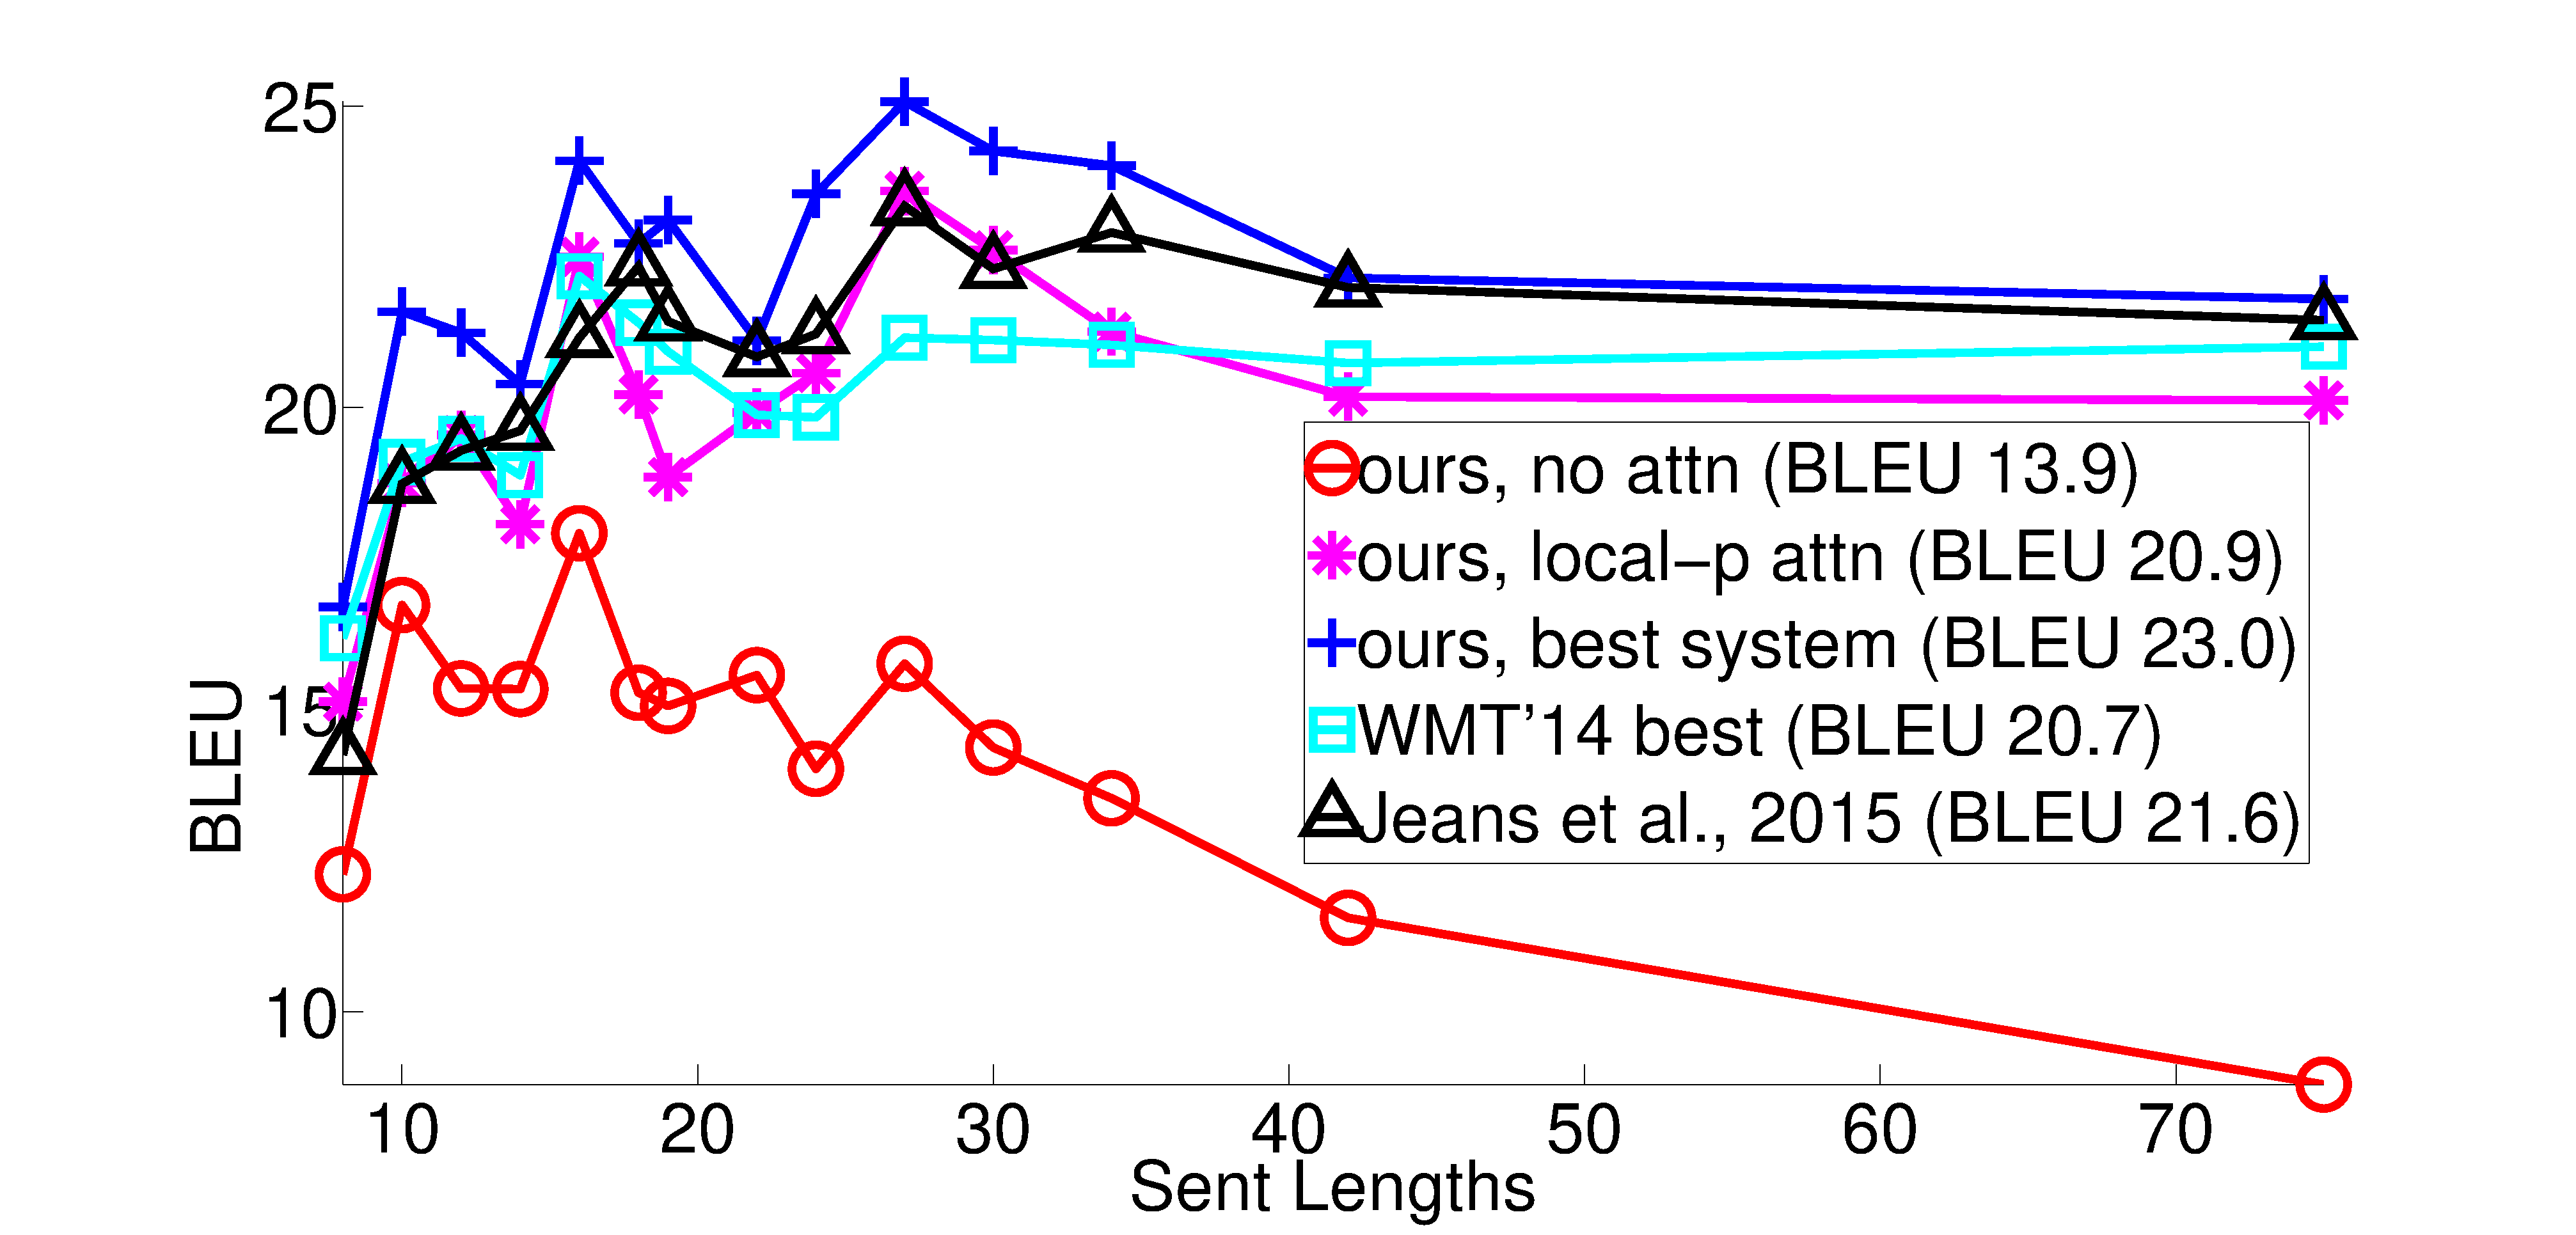
\includegraphics[width=0.7\textwidth, clip=true, trim=120 0 70 0]{img/4-length} % , angle=-90
\caption[Length Analysis]{{\bf Length Analysis} -- translation qualities of different
systems as sentences become longer.
} 
\label{f:length}
\end{figure}

\subsection{Choices of Attentional Architectures}
I examine different attention models ({\it global, local-m, local-p}) and different
alignment functions ({\it location, dot, general, concat}) as described in
Section~\ref{sec:attn}. Due to limited
resources, I cannot run all the possible combinations.
However, results in Table~\ref{t:attnChoices} do give us some idea about
different choices. 
The {\it location-based} function does not learn good
alignments: the {\it global (location)} model can only obtain a small
gain when performing unknown word replacement compared to using other alignment
functions.\footnote{There is a subtle difference in how I retrieve alignments
for the different alignment functions. At time step $t$ in which I receive
$\tgt{t-1}$ as input and then compute $\hi, \al, \co$, and $\hs$ before
predicting $\tgt{t}$, the alignment vector $\al$ is used as alignment
weights for (a) the predicted word $\tgt{t}$ in the {\it location-based}
alignment functions and (b) the input word $\tgt{t-1}$ in the {\it content-based}
functions.}
For {\it content-based} functions, my implementation {\it concat} does not yield good performances
and more analysis should be done to understand the
reason.\footnote{With {\it concat}, the perplexities achieved by different models are 6.7 (global), 7.1
(local-m), and 7.1 (local-p). Such high perplexities could be due to the fact
that I simplify the matrix \MB{W_a} to set the part that corresponds to $\his$
to identity.} It is interesting to observe that {\it dot} works
well for the global attention and {\it general} is better for the local
attention.
Among the different models, the local attention model with predictive alignments ({\it
local-p}) is best, both in terms of perplexities and BLEU.

\begin{table}
\centering
%\resizebox{8cm}{!}{
\begin{tabular}{l|r|c|c}
\multirow{ 2}{*}{\bf{System}} & \multirow{ 2}{*}{\bf{Ppl}} &
\multicolumn{2}{c}{{\bf BLEU}}\\
\cline{3-4}
& & Before & After unk \\
  \hline
global (location) & 6.4 & 18.1 & 19.3 (+1.2) \\
%global (concat) & 6.7 & xx & xx (+xx) \\
global (dot) & 6.1 & 18.6 & 20.5 (+1.9) \\
global (general) & 6.1 & 17.3 & 19.1 (+1.8) \\
  \hline
local-m (dot) & $>$7.0 & x & x \\
local-m (general) & 6.2 & 18.6 & 20.4 (+1.8) \\
  \hline
local-p (dot) & 6.6 & 18.0 & 19.6 (+1.9) \\
local-p (general) & {\bf 5.9} & {\bf 19} & {\bf 20.9 (+1.9)} \\
\end{tabular}
%}
\caption[Attentional Architectures]{{\bf Attentional Architectures} -- performances of different
attentional
models. I trained two local-m (dot) models; both have
ppl $>7.0$.}
\label{t:attnChoices}
\end{table}

\subsection{Alignment Quality}
A by-product of attentional models are word alignments. While \cite{bog15}
visualized alignments for some sample sentences and 
observed gains in translation quality as an indication of a working attention
model, no work has assessed the alignments learned as a whole. In contrast, I
set out to evaluate the alignment quality using the alignment error rate (AER)
metric.

\begin{table}
  \begin{center}
    \begin{tabular}{c c}
      {\bf Method} & {\bf AER} \\
      \hline
      global (location) & $0.39$ \\
      local-m (general)  & $0.34$ \\
      local-p (general) & $0.36$ \\
      \hdashline
      ensemble & $0.34$ \\
      \hline
      Berkeley Aligner & $0.32$ \\
    \end{tabular}
  \end{center}
  \caption[AER scores]{{\bf AER scores} -- results of various models on the RWTH
  English-German alignment data.}
  \label{t:alignment}
\end{table}

Given the gold alignment data provided by RWTH for 508 English-German
Europarl sentences, I ``force'' decode my attentional models to
produce translations that match the references. I extract only one-to-one
alignments by selecting the source word with the highest alignment
weight per target word. Nevertheless, as shown in Table~\ref{t:alignment}, I was able to achieve AER scores
comparable to the one-to-many alignments obtained by the Berkeley aligner
\cite{liang06alignment}.\footnote{I concatenate the 508 sentence pairs with 1M
sentence pairs from WMT and run the Berkeley aligner.}

I also found that the alignments produced by local attention models achieve
lower AERs than those of the global one. The AER obtained by the ensemble, while
good, is not better than the local-m AER, suggesting the well-known
observation that AER and translation scores are not well correlated \cite{fraser07}.

\subsection{Alignment Visualization}
I visualize the alignment weights produced by my different attention
models in Figure~\ref{i:alignment}. The visualization of the local
attention model is much sharper than that of the global one. This contrast matches
my expectation that local attention is designed to only focus on a subset of
words each time. Also, since I
translate from English to German and reverse the source English sentence, the white strides
at the words {\it ``reality''} and {\it ``.''} in the global attention model reveals an
interesting access pattern: it tends to refer back to the beginning of the
source sequence. 

Compared to the alignment visualizations in \cite{bog15}, my 
alignment patterns are not as sharp as theirs. Such difference could possibly be due to
the fact that translating from English to German is
harder than translating into French as done in \cite{bog15},
which is an interesting point to examine in future work.

\begin{figure*}
  \begin{center}
    \includegraphics[width=0.48\textwidth]{img/4-align4.eps}
    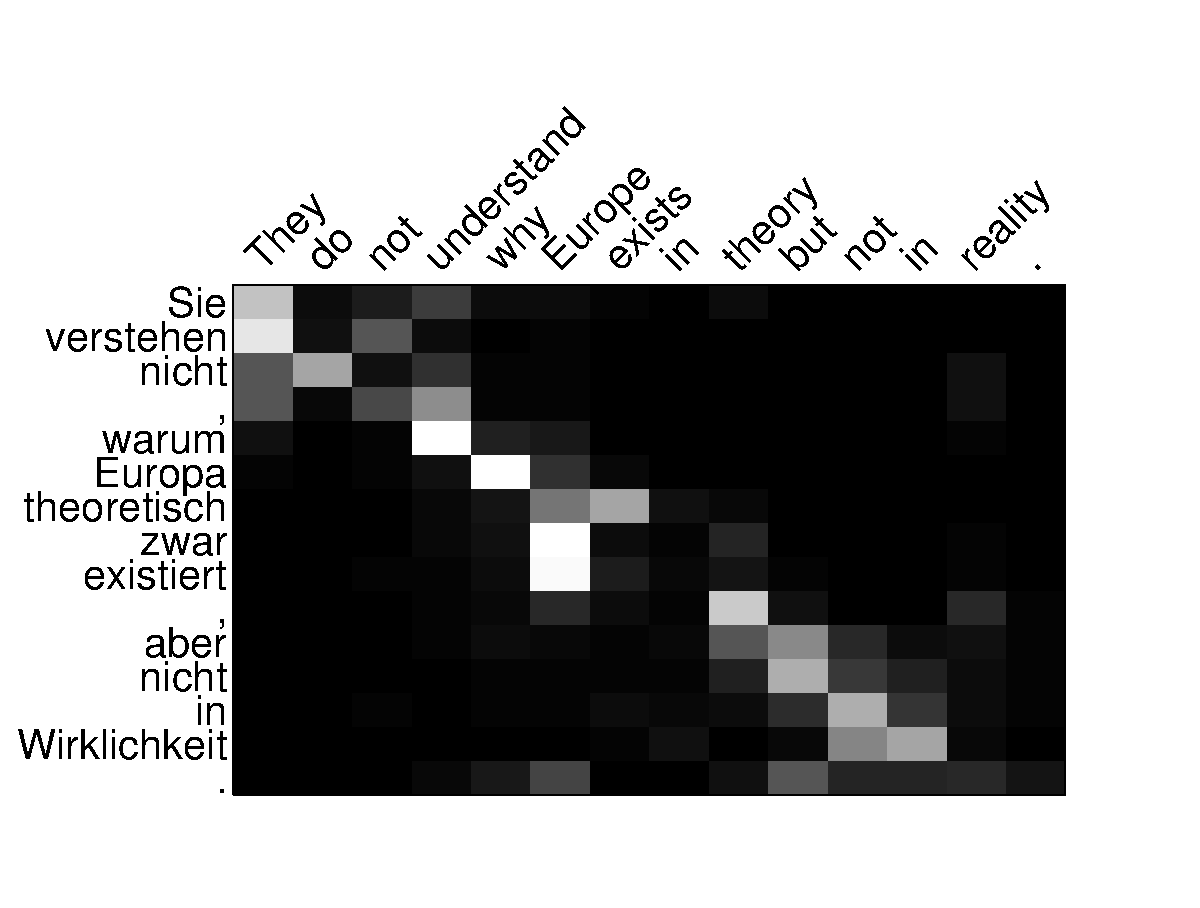
\includegraphics[width=0.48\textwidth]{img/4-align2.eps}
    \includegraphics[width=0.48\textwidth]{img/4-align1.eps}
    \includegraphics[width=0.48\textwidth]{img/4-alignGold.eps}
  \end{center}
  \caption[Alignment visualizations]{{\bf Alignment visualizations} -- shown are images of the attention
  weights learned by various models: (top left) global, (top right)
  local-m, and (bottom left) local-p. The {\it gold} alignments are
  displayed at the bottom right corner.
  }
  \label{i:alignment}
\end{figure*}

\subsection{Sample Translations}
\label{sec:sample}
I show in Table~\ref{t:sample} sample translations in both directions. It it
appealing to observe the effect of attentional models in correctly translating
names such as ``Miranda Kerr'' and ``Roger Dow''. Non-attentional models, while producing sensible names from a language
model perspective, lack the direct connections from the source side to make
correct translations. % as with the case of attention-based NMT systems. 
I also observed an interesting case in the second
example, which requires translating the {\it doubly-negated} phrase, ``not incompatible''.
The attentional model correctly produces ``nicht $\dots$ unvereinbar'';
whereas the non-attentional model generates ``nicht vereinbar'', meaning
``not compatible''.\footnote{The reference uses a more fancy translation of
``incompatible'', which is ``im Widerspruch zu etwas stehen''. Both models, however, failed to translate ``passenger
experience''.} The attentional
model also demonstrates its superiority in translating long sentences as in
the last example.
\begin{table*}[tbh!]
\centering
\resizebox{15cm}{!}{
\begin{tabular}{c|p{15cm}}
\multicolumn{2}{l}{{\bf English-German translations}}\\
  \hline
src & Orlando Bloom and Miranda Kerr still love each other \\
  \hline
ref & Orlando Bloom und \correct{Miranda Kerr} lieben sich noch immer \\
  \hline
{\it best} & Orlando Bloom und \correct{Miranda Kerr} lieben einander noch immer . \\
  \hline
base & Orlando Bloom und \wrong{Lucas Miranda} lieben einander noch immer .\\
  \hline
  \hline
src & $''$ We $'$ re pleased the FAA recognizes that an enjoyable passenger experience is not incompatible with safety and security , $''$ said Roger Dow , CEO of the U.S. Travel Association . \\
  \hline
ref & `` Wir freuen uns , dass die FAA erkennt , dass ein angenehmes
Passagiererlebnis nicht im Widerspruch zur Sicherheit steht '' , sagte
\correct{Roger Dow} , CEO der U.S. Travel Association . \\
  \hline
{\it best} & $''$ Wir freuen uns , dass die FAA anerkennt , dass ein angenehmes ist
nicht mit Sicherheit und Sicherheit \correct{unvereinbar} ist $''$ , sagte \correct{Roger
Dow} , CEO der US - die . \\
  \hline
base & $''$ Wir freuen uns \"{u}ber die $<$unk$>$ , dass ein $<$unk$>$ $<$unk$>$
mit Sicherheit nicht \wrong{vereinbar} ist mit Sicherheit und Sicherheit $''$ ,
sagte \correct{Roger} \wrong{Cameron} , CEO der US - $<$unk$>$ . \\
  \hline
  \hline
\multicolumn{2}{l}{{\bf German-English translations}}\\
  \hline
src & In einem Interview sagte Bloom jedoch , dass er und Kerr sich noch immer lieben . \\
  \hline
ref & However , in an interview , Bloom has said that he and \correct{Kerr} still love each other . \\
  \hline
{\it best} & In an interview , however , Bloom said that he and \correct{Kerr} still love . \\
  \hline
base & However , in an interview , Bloom said that he and \wrong{Tina} were still $<$unk$>$ . \\
  \hline
  \hline
src & Wegen der von Berlin und der Europ\"{a}ischen Zentralbank verh\"{a}ngten strengen Sparpolitik in Verbindung mit der Zwangsjacke , in die die jeweilige nationale Wirtschaft durch das Festhalten an der gemeinsamen W\"{a}hrung gen\"{o}tigt wird , sind viele Menschen der Ansicht , das Projekt Europa sei zu weit gegangen \\ 
  \hline
ref & The \correct{austerity imposed by Berlin and the European Central Bank , coupled with the straitjacket} imposed on national economies through adherence to the common currency , has led many people to think Project Europe has gone too far .\\
  \hline
{\it best} & Because of the strict \correct{austerity measures imposed by Berlin
and the European Central Bank in connection with the straitjacket} in which the
respective national economy is forced to adhere to the common currency , many
people believe that the European project has gone too far . \\
  \hline
base & Because of the pressure \wrong{imposed by the European Central Bank and the Federal Central Bank with the strict austerity} imposed on the national economy in the face of the single currency , many people believe that the European project has gone too far .\\
\end{tabular}
}
\caption[Sample translations]{{\bf Sample translations} -- %examples in both translation directions.
for each example, I show the source ({\it src}), the human translation ({\it
ref}), the translation from my best model ({\it best}), and the
translation of a non-attentional model ({\it base}).  I italicize some
\correct{correct} translation segments and highlight a few \wrong{wrong} ones in
bold.} % See Appendix~\ref{sec:sample} for detailed descriptions.}
\label{t:sample}
\end{table*}

\section{Conclusion}
\label{sec:conclude}
In this chapter, I propose two simple and effective attentional mechanisms for
neural machine translation: the {\it global} approach which always looks at all
source positions and the {\it local} one that only attends to a subset of source
positions at a time. I test the effectiveness of my models in the WMT
translation tasks between English and German in both directions. 
My local attention yields large gains of up to
$\attngain{}$ BLEU over non-attentional models that already incorporate known
techniques such as dropout. For the English to German translation direction, my
ensemble model has established new state-of-the-art
results for both WMT'14 and WMT'15.

I have compared various alignment functions and shed light on which functions
are best for which attentional models.
My analysis shows that attention-based NMT models are superior to
non-attentional ones in many cases, for example in translating names and
handling long
sentences.


\chapter{Hybrid Models}
\label{c:hybrid}
Neural Machine Translation (NMT) is a simple new architecture for getting
machines to translate. At its core, NMT is a single deep 
neural network that is trained end-to-end with several advantages such as
simplicity and generalization. Despite being relatively new, NMT has already
achieved state-of-the-art translation results for several language pairs 
such as English-French \cite{luong15}, English-German
\cite{jean15,luong15attn,luong15iwslt}, and English-Czech \cite{jean15wmt}. 
\begin{figure}%[tbh]
\centering
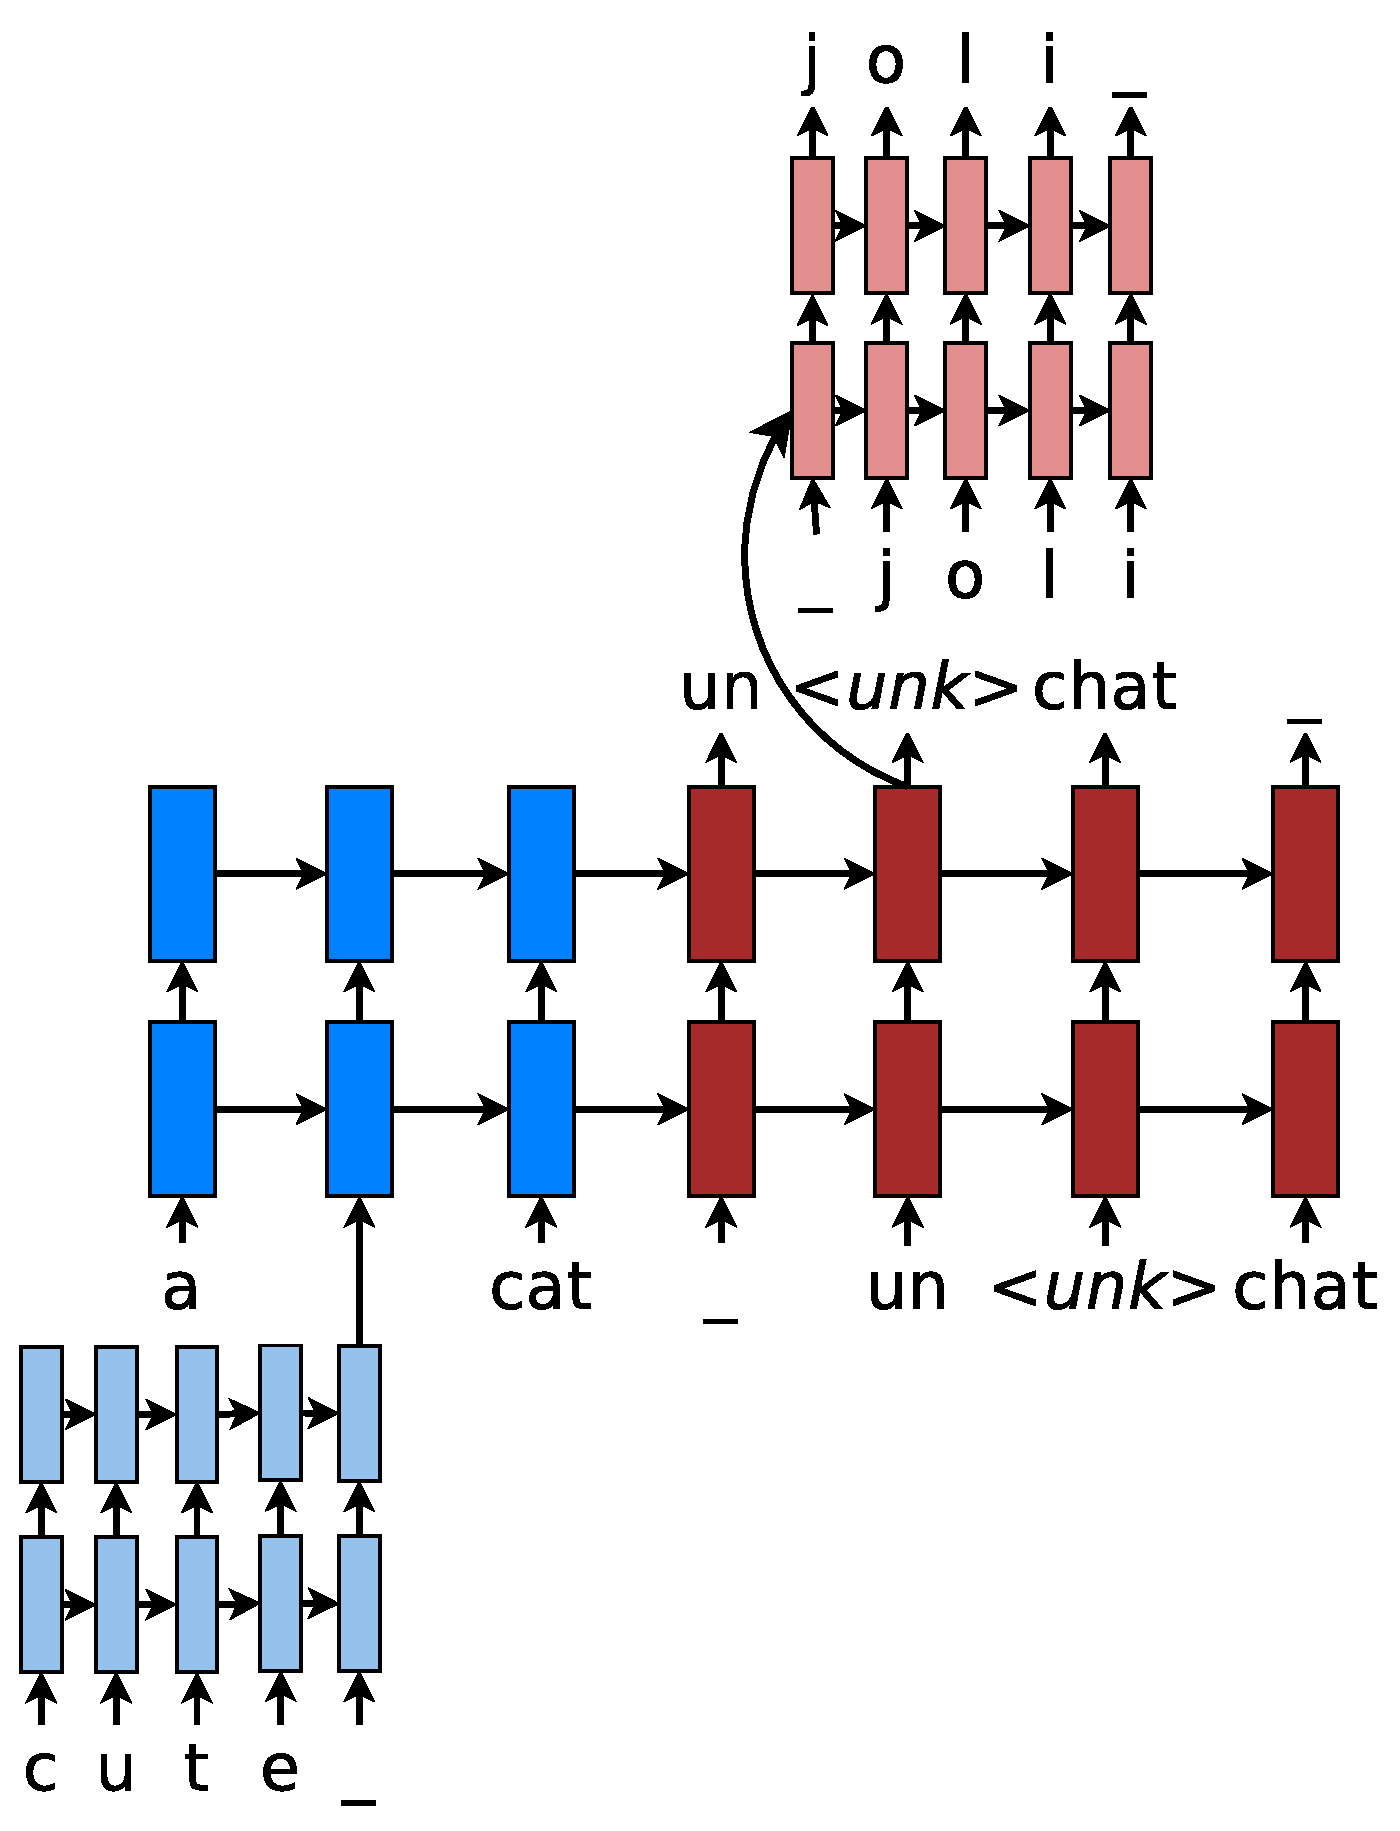
\includegraphics[width=0.6\textwidth, clip=true, trim= 0 0 0 0]{img/5-nmt_hybrid}
\caption[Hybrid NMT]{{\bf Hybrid NMT} -- example of a word-character model for translating
\word{a cute cat} into \word{un
joli chat}. Hybrid NMT translates at the word level. For rare tokens,
the character-level components build source representations
and recover target \unk{}. \word{\_} marks sequence
boundaries.}
\label{f:hybrid}
\end{figure}

While NMT offers many advantages over traditional phrase-based approaches, such as
small memory footprint and simple decoder implementation, nearly all previous
work in NMT has used quite restricted vocabularies, crudely treating all other
words the same with an \unk{} symbol. Sometimes, a post-processing step that
patches in unknown words is introduced to alleviate this problem. %For example,
\newcite{luong15} propose to annotate occurrences of target \unk{} with positional information to
track their alignments, after which simple word dictionary
lookup or identity copy can be performed to replace \unk{} in the translation.
\newcite{jean15} approach the problem similarly but obtain the alignments for unknown
words from the attention mechanism. We refer to these as the {\it
unk replacement} technique.

Though simple, these approaches ignore several important
properties of languages. First, {\it monolingually}, words are morphologically
related; however, they are currently treated as independent entities. This is
problematic as pointed out by
\newcite{luong13}: neural networks can learn good
representations for frequent words such as \word{distinct}, but fail for
rare-but-related words like \word{distinctiveness}. Second, {\it crosslingually},
languages have different alphabets, so one cannot na\"{i}vely memorize all
possible surface word translations such as name transliteration between 
\word{Christopher} (English) and \word{Kry\u{s}tof} (Czech). See more on this problem
in \cite{sennrich16sub}.

To overcome these shortcomings, we propose a novel {\it hybrid} architecture for NMT
that translates mostly at the word level and consults the character
components for rare words when necessary. As illustrated in
Figure~\ref{f:hybrid}, our hybrid model consists of a word-based NMT that
performs most of the translation job, except for the two (hypothetically) rare words,
\word{cute} and \word{joli}, that are handled separately. On the {\it source}
side, representations for rare words, \word{cute}, are
computed on-the-fly using a deep recurrent neural network that operates at the
character level. On the {\it target} side, we have a separate model that
recovers the surface forms, \word{joli}, of \unk{} tokens character-by-character.
These components are learned jointly end-to-end, removing the need for a separate
unk replacement step as in current NMT practice.

Our hybrid NMT offers a twofold advantage: it is much faster and easier to
train than character-based models; at the same time, it never produces unknown
words as in the case of word-based ones.
We demonstrate at scale that on the WMT'15 English to
Czech translation task, such a hybrid approach provides
an additional boost of +$\gain{}$ BLEU points over models 
that already handle unknown words.
We achieve a new state-of-the-art result with
$\ensbleu{}$ BLEU score.
Our analysis demonstrates that our character models can successfully learn to not
only generate well-formed words for Czech, a
highly-inflected language with a very complex vocabulary, but also build correct
representations for English source words.

We provide code, data, and models at \url{http://nlp.stanford.edu/projects/nmt}.

\section{Related Work}
There has been a recent line of work on end-to-end character-based neural models
which achieve good results for part-of-speech tagging \cite{santos14,ling15function},
dependency parsing \cite{ballesteros15}, text classification
\cite{zhang15}, speech recognition \cite{chan16,bahdanau16}, and language
modeling \cite{kim16,rafal16}. However, success has not been shown for
cross-lingual tasks such as machine translation.\footnote{Recently,
\newcite{ling15char} attempt character-level NMT; however,
the experimental evidence is weak. The authors demonstrate only small
improvements over word-level baselines and acknowledge that there are no differences of
significance. Furthermore, only small datasets were used without
comparable results from past NMT work.}
\newcite{sennrich16sub} propose to segment words into smaller units and
translate just like at the word level, which does not learn to understand
relationships among words.

Our work takes inspiration from \cite{luong13} and 
\cite{li15}. Similar to the former, we build representations for rare words
on-the-fly from subword units. However, we utilize recurrent neural networks
with characters as the basic units; whereas \newcite{luong13} use recursive neural
networks with morphemes as units, which requires existence of a
morphological analyzer. In comparison with \cite{li15}, our hybrid architecture
is also a hierarchical sequence-to-sequence model, but operates at a different
granularity level, word-character. In contrast, \newcite{li15} build
hierarchical models at the sentence-word level for paragraphs and documents.

\section{Background \& Our Models}
\label{sec:nmt}
Neural machine translation aims to directly model the conditional probability $p(\tgt{}|\src{})$ of translating
a source sentence, $\src{1},\ldots,\src{n}$, to a target sentence, $\tgt{1},\ldots,\tgt{m}$.
It accomplishes this goal through an {\it encoder-decoder} framework
\cite{kal13,sutskever14,cho14}. The {\it encoder} computes a representation $\MB{s}$
for each source sentence. Based on that source representation,
the {\it decoder} generates a translation, one target word at a time, and hence,
decomposes the log conditional probability as:
\begin{equation}
\log p(\tgt{}|\src{}) = \sum_{t=1}^m \nolimits \log
p\open{\tgt{t}|\tgt{<t},\MB{s}}
\label{e:s2s}
\end{equation}

A natural model for sequential data is the recurrent
neural network (RNN), used by most of the recent NMT work.
Papers, however, differ in terms of: (a) architecture -- from unidirectional, to
bidirectional, and deep multi-layer RNNs; and (b) RNN type -- which are long
short-term memory (LSTM)
\cite{lstm97} and the gated recurrent unit \cite{cho14}. 
All our models utilize the {\it deep multi-layer} architecture with {\it
LSTM} as the recurrent unit; detailed formulations are in \cite{zaremba14}.

%A natural choice to model such a decomposition in the decoder is to use a
%recurrent neural network (RNN) architecture, which most of the recent NMT work have in common. They,
%however, differ in terms of the RNN architectures used and how the encoder computes the source representation $\MB{s}$.
%%, e.g., vanilla RNN, long-short term memory (LSTM) \cite{lstm97} or gated recurrent units \cite{cho14}
%\newcite{kal13} used an RNN with the vanilla RNN unit for the decoder and a
%convolutional neural network for encoding the source. On
%the other hand, \newcite{sutskever14,luong15,luong15attn} built deep RNNs with the Long Short-Term Memory (LSTM) unit
%\cite{lstm97} for both the encoder and the decoder. \newcite{cho14,bog15,jean15} all adopted an
%LSTM-inspired hidden unit, the gated recurrent unit (GRU), and used bidirectional
%RNNs for the encoder.
%%\footnote{They all used a single RNN layer except for the latter two
%%works which utilized a bidirectional RNN for the encoder.}

Considering the top recurrent layer in a deep LSTM, 
with $\hd{t}$ being the current target hidden state as in Figure~\ref{f:attn}, one can compute the probability of decoding each target word $y_t$ as:
\begin{equation}
p\left(\tgt{t}|\tgt{<t},\MB{s}\right) = \softmax\open{\hd{t}}
\label{e:softmax}
\end{equation}

For a parallel corpus $\mathbb{D}$, we train our model by minimizing the below
cross-entropy loss:
\begin{equation}
J = \sum_{(\src{},\tgt{}) \in \mathbb{D}} \nolimits -\log p(\tgt{}|\src{})
\label{e:obj}
\end{equation}

\noindent {\bf Attention Mechanism} -- 
%Another important difference between NMT work lies in what constitutes the
%input representation $\MB{s}$.
The early NMT approaches \cite{sutskever14,cho14}, which we have described above, use only the last encoder state
 to initialize the decoder, i.e., setting the input representation $\MB{s}$ in
 \eq{e:s2s} to $[\hb{n}]$. Recently, \newcite{bog15} propose an {\it attention
 mechanism}, a form of random access memory for NMT to 
cope with long input sequences.
%This is accomplished by setting
%$\MB{s}$ to be the set of encoder hidden states already computed. % $[\hb{1}, \dots, \hb{n}]$
\newcite{luong15attn} further extend the attention mechanism to different
scoring functions, used to compare source and target
hidden states, as well as different
strategies to place the attention.
%{\it global} -- utilize all source hidden
%states at all target timesteps and {\it local} -- focus on a small subset of
%source hidden states per target timestep.
In all our models, we utilize the {\it global} attention mechanism and the {\it
bilinear form} for the attention scoring function similar to 
\cite{luong15attn}.

\begin{figure}
\centering
%\psgrid
\rput(4.3,6.5){$\tgt{t}$}
\rput(1.4,5.6){$\co$}
\rput(0.8,3.1){$\hb{1}$}
\rput(2.9,3.1){$\hb{n}$}
\rput(4.9,3.1){$\hd{t}$}
\rput(4.9,6.0){$\hs$}
%\rput(4.0,3.8){$\hd{t-1}$}
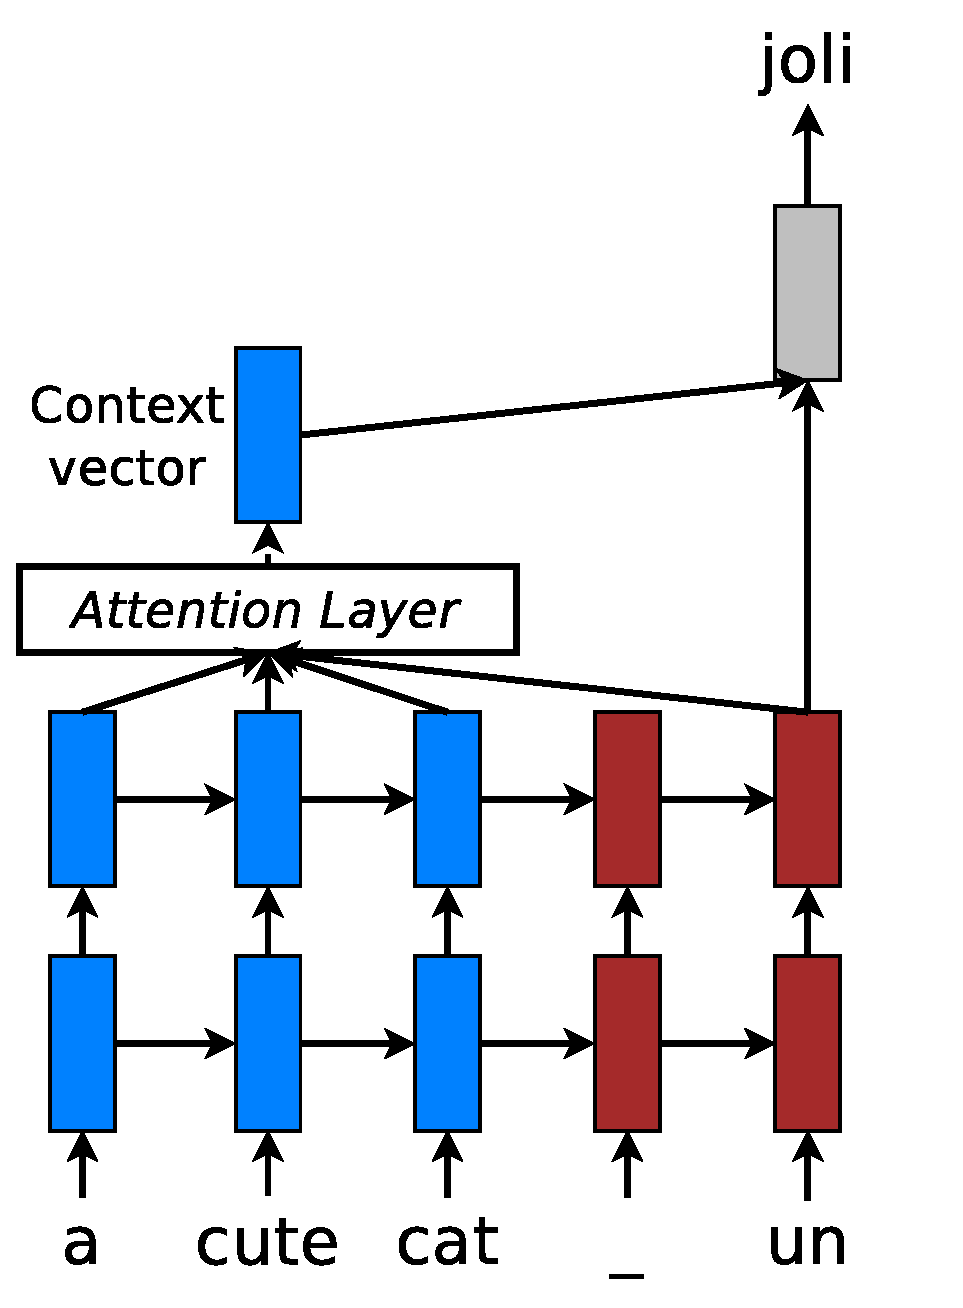
\includegraphics[width=0.33\textwidth, clip=true, trim= 0 0 0 0]{img/5-attn} % , angle=-90
\caption[Attention mechanism]{{\bf Attention mechanism}.
% -- shown are the two steps of the attention mechanism described in \cite{luong15attn}
%: first, compute a 
%{\it context vector} $\co$ based on the current target hidden state $\hd{t}$ and all the source hidden
%states $[\hb{1}, \dots, \hb{n}]$; second, use the context vector as an
%additional input to derive
%the {\it attentional} vector $\hs$.
} 
\label{f:attn}
\end{figure}

Specifically, we set $\MB{s}$ in \eq{e:s2s} to
the set of source hidden states at the top layer, $[\hb{1}, \dots, \hb{n}]$. 
As illustrated in Figure~\ref{f:attn}, the attention mechanism consists of two stages: (a) {\it
context vector} -- the current hidden state $\hd{t}$ is compared with
individual source hidden states in $\MB{s}$ to learn an alignment vector, which
is then used to compute the context vector $\co$ as a weighted average of
$\MB{s}$; and (b) {\it
attentional hidden state} -- the context vector $\co$ is then used to derive a
new attentional hidden state:
\begin{equation}
\hs = \tanh(\W{}[\co; \hi])
\label{e:hs}
\end{equation} 
The attentional vector $\hs$ then replaces $\hd{t}$ in \eq{e:softmax} in
predicting the next word.

\section{Hybrid Neural Machine Translation}
\label{sec:hybrid}
Our hybrid architecture, illustrated in Figure~\ref{f:hybrid}, leverages the power of both words
and characters to achieve the goal of open vocabulary NMT. The core of the
design is a {\it word}-level NMT with the advantage of being fast and easy to
train.
%, whereas purely character-based NMT has to deal with very
%long sequences. 
The {\it character} components empower the 
word-level system with the abilities to compute any source word representation on the fly from 
characters and to recover character-by-character unknown target words
originally produced as \unk{}.

\subsection{Word-based Translation as a Backbone}
\label{subsec:hybrid_word}
%\begin{figure}%[tbh]
%\centering
%\includegraphics[width=0.4\textwidth, clip=true, trim= 0 0 0 0]{nmt_word.\imgExt}
%\caption{{\bf Word-based NMT} -- the backbone of our hybrid architecture. Boxes
%mark the character-level components for: (a) computing source word
%representations and (b) generating target words.}
%%to take advantages of the
%%original forms of the rare words.}
%\label{f:word}
%\end{figure}

The core of our hybrid NMT is a deep LSTM encoder-decoder that translates at
the {\it word} level as described in Section~\ref{sec:nmt}. We maintain a
vocabulary of $|V|$ frequent words for each language. Other words not inside these
lists are represented by a universal symbol \unk{}, one per language.
We translate just like a word-based NMT system with respect to these source and
target vocabularies, except for cases that involve \unk{} in the source input or 
the target output. These correspond to the character-level components 
%that we will expand next to accomplish the full architecture as 
illustrated in Figure~\ref{f:hybrid}.
%and are highlighted by the two boxes in 
%Figure~\ref{f:word}.
%Note that we leave \unk{} on the target input which helps simplify the training
%and testing phases as detailed in Section~\ref{subsubsec:strategy}.

A nice property of our hybrid approach is that by varying the vocabulary size,
 one can control how much to blend the
word- and character-based models; hence, taking the best of both
worlds. 
%We illustrate that unified view in Figure~\ref{f:vocabulary}.


\subsection{Source Character-based Representation}
\label{subsec:src}
%We now describe box (a) in Figure~\ref{f:word}. 
In regular word-based
NMT, for all rare words outside the source vocabulary, one feeds the
universal embedding representing \unk{} as input to the encoder. This is
problematic because it discards valuable information about the source word. To
fix that, we learn a deep LSTM model over characters
of source words. 
%In our running example, % for the word \word{cute}, 
For example, in Figure~\ref{f:hybrid}, we run
our deep character-based LSTM over `c', `u', `t', `e', and `\_' (the boundary
symbol). The final hidden state at the top layer will be used as the on-the-fly
representation for the current rare word.
%as illustrated in the bottom-left part of Figure~\ref{f:hybrid}.

The layers of the deep character-based LSTM are always initialized with {\it
zero} states. One might propose to connect hidden
states of the word-based LSTM to the character-based model; however, we chose this design
for various reasons. First, it simplifies the architecture. Second, it allows
for efficiency through {\it precomputation}: before each mini-batch, we can compute
representations for rare source words all at once. All instances of the same
word share the same embedding, so the computation is per {\it type}.\footnote{While \newcite{ling15char} found that it is slow and difficult to train
source character-level models and had to resort to pretraining, we demonstrate
later that we can train our deep character-level LSTM %in the experiment section 
perfectly fine in an end-to-end fashion.} 

%This approach is inspired by the work
%of \cite{luong13} which also computes on-the-fly representations
%for rare words. Their work, however, is different from ours in that the representations
%are derived from morphemes, with recursive neural networks, and for
%the language modeling task.

%\begin{figure}%[tbh]
%\centering
%\includegraphics[width=0.45\textwidth, clip=true, trim= 0 0 0 0]{vocabulary.\imgExt}
%\caption{{\bf A unified view of hybrid NMT} -- as the word vocabulary size
%approaches zero, we obtain character-based NMT; whereas, large vocabulary
%sizes lead to word-based NMT.}
%\label{f:vocabulary}
%\end{figure}


\subsection{Target Character-level Generation}
\label{subsec:tgt}
%Next, we describe box (b) in Figure~\ref{f:word}.
General word-based NMT allows generation of \unk{} in the target output.
%will accept the fact when generating target words, \unk{} can be emitted. 
Afterwards, there is usually a post-processing step that handles
these unknown tokens by utilizing the
alignment information derived from the attention mechanism and then performing
simple word dictionary lookup or identity copy \cite{luong15attn,jean15}. 
While this approach works, it suffers from various problems such as alphabet
mismatches between the source and target vocabularies and multi-word
alignments.
%, as detailed in Section~\ref{subsec:rare}. 
Our goal is to address all
these issues and create a
coherent framework that handles an unlimited output vocabulary.
%virtually has the ``post-processing'' step baked in and
%learned automatically end-to-end. 

Our solution is to have a separate deep LSTM that ``translates'' at the
character level given the current word-level state. We train our system such
that whenever the word-level NMT
produces an \unk{}, we can consult this character-level decoder to recover the correct surface form of the
unknown target word. This is illustrated in Figure~\ref{f:hybrid}.
The training objective in \eq{e:obj} now becomes: %consists of two components:
\begin{equation}
J = J_{w} + \alpha J_{c}
\label{e:char_obj}
\end{equation}
Here, $J_{w}$ refers to the usual loss of the word-level NMT; in
our example, it is the sum of the negative log likelihood of
generating $\{\mbox{``un'', ``\unk{}'', ``chat'', ``\_''}\}$. The remaining component $J_c$
corresponds to the loss incurred by the character-level 
decoder when predicting characters, e.g., $\{\mbox{`j', `o', `l', `i',
`\_'}\}$, of those rare words not in the
target vocabulary. 
%In our running example, the predicted characters are .


\paragraph{Hidden-state Initialization} %Separated-path Target Generation}
\label{subsubsec:h}
Unlike the source character-based representations, which are
context-independent, the target character-level generation requires the
current word-level context to produce meaningful translation.
This brings up an important
question about what can best represent the current context so as to
initialize the character-level decoder. We answer this question in the context
of the attention mechanism ($\S$\ref{sec:nmt}). 
%, which has now become the defacto standard in NMT.

The final vector $\hs$, just before the
softmax as shown in Figure~\ref{f:attn}, seems to be a good candidate to initialize the character-level decoder.
The reason is that $\hs$ combines
information from both the context vector $\co$ and the top-level recurrent
state $\hi$. We refer to it later in our
experiments as the \textit{same-path} target generation approach.

On the other hand, the same-path approach worries us because all vectors $\hs$
used to seed the character-level decoder might have similar values, leading to
the same character sequence being produced.
The reason is because $\hs$ is directly used in the softmax, \eq{e:softmax}, to predict the same \unk{}.
That might pose some challenges for the model to learn useful representations
that can be used to accomplish two tasks at the same time, that is to predict
\unk{} and to generate character sequences.
To address that concern, we propose another approach called
the \textit{separate-path} target generation.

Our separate-path target generation approach works as follows. We mimic the
process described in \eq{e:hs} to create a counterpart vector $\hc$ that will be
used to seed the character-level decoder:
\begin{equation}
\hc = \tanh(\Wc[\co; \hi])
\label{e:hc}
\end{equation} 
Here, $\Wc$ is a new learnable parameter matrix, with which we
hope to release $\W{}$ from the pressure of having to extract information
relevant to both the word- and character-generation processes.
%This approach is illustrated in Figure~\ref{f:tgtGen}.
Only the hidden
state of the first layer is initialized as discussed above. The other components
in the character-level decoder such as the
LSTM cells of all layers and the hidden states of higher layers, all start with zero values.

%\begin{figure}%[tbh]
%\centering
%%\psgrid
%\rput(1.5,4.0){$\co$}
%\rput(2.6,3.75){$\Wc$}
%\rput(3.07,4.9){$\hc$}
%\rput(4.4,3.7){$\Ww$}
%\rput(5.1,1.5){$\hi$}
%\rput(5.1,4.9){$\hs$}
%%\rput(0.9,1.9){$\his$}
%\includegraphics[width=0.35\textwidth, clip=true, trim= 0 0 0 0]{tgtGen.\imgExt}
%\caption{{\bf Target generation for rare words} -- the backbone of our hybrid architecture. Boxes
%mark the character-level components for: (a) computing source word
%representations and (b) generating target words.}
%%to take advantages of the
%%original forms of the rare words.}
%\label{f:tgtGen}
%\end{figure}

Implementation-wise, the computation in the
character-level decoder is done per word {\it token} instead of per {\it type} as in the source
character component ($\S$\ref{subsec:src}). 
This is because of the context-dependent nature of the decoder.
%\footnote{For memory efficiency, the character-level backward pass can be executed right
%after the character-level forward pass
%and we can split these computations into
%mini-batches if the number of \unk{} is large.}

%initialized hidden states are different across time steps and across sentences even if the surface
%forms to be generated are the same. 

%For speed efficiency, we run a forward pass
%over the word-level decoder first. Then, we invoke, in batch mode, a forward
%pass over the character-level decoder for the surface forms of all the \unk{} tokens.

\paragraph{Word-Character Generation Strategy}
\label{subsubsec:strategy}
With the character-level decoder, we can view the final hidden states as representations for
the surface forms of unknown tokens and could have fed these to the next
time step. However, we chose not to do so for the efficiency reason explained
next; instead, \unk{} is fed to the word-level decoder
``as is'' using its corresponding word embedding.
% as illustrated in Figure~\ref{f:word}. 

During {\it training}, this design choice decouples all executions over \unk{} instances of the
character-level decoder as soon the word-level NMT
completes. As such, the forward and backward passes of the character-level
decoder over rare words can be invoked in batch mode. At {\it test} time,
our strategy is to first run a beam search decoder at the word level to
find the best translations given by the
word-level NMT. Such translations contains \unk{} tokens, so we utilize our
character-level decoder with beam search to generate actual words for these \unk{}.
%We aggregate the word- and charater-level
%decoding scores according to the formula in \eq{e:char_obj} and find the best
%translation according to the combined scores.
% \todo{Implement this scheme to take
%into account the combined scores.}

\hide{
\subsection{Sampling for Better Rare Word Learning}
When the vocabulary size is large, i.e., when our hybrid NMT system is closer to a
word-based one, it is often the case that a frequent word appears in
the vocabulary but not its derived forms. In
these cases, character-level models will only be able to learn to represent
rare words, e.g., ``distinctiveness'', but not their related but frequent forms, e.g.,
``distinct''. This implies
that our hybrid NMT may have ignored valuable information about the
relationship among many words. 

To tackle this problem, we
propose a sampling approach to occasionally select frequent words in a
training mini-batch and view them as rare
words so that character-level models can learn from them.
The number of frequent words we sample per 
mini-batch is counted by {\it type} on the source side  and by {\it
token} on the target side. This is in accordance with how we sample rare words
to build character-based representations and perform character-level generation in
Section~\ref{subsec:src} and \ref{subsec:tgt} respectively. 

As a result of this sampling approach, each
frequent word in the {\it source} vocabulary will have two
representations, one from the character-based model and one from the
word embeddings. For these two representations to cooperate with the recurrent
connections, the source character-level model is virtually encouraged to produce
similar word embeddings. \todo{Test this by visualization.} On the {\it target}
side, this approach helps force the word-level NMT to produce relevant top
hidden states that can readily be used to generate sensible character sequences
even if the target words to be predicted are not \unk{}.
}

\section{Experiments}
\label{sec:exp}
We evaluate the effectiveness of our models on the publicly available WMT'15
translation task from English into Czech with 
{\it newstest2013} (3000 sentences) as
a development set % to select our hyperparameters. 
and {\it newstest2015} (2656 sentences) as a test set. Two metrics are used: case-sensitive NIST BLEU \cite{Papineni02bleu}
and \chr{} \cite{chrf}.\footnote{For NIST BLEU, we first run
\texttt{detokenizer.pl} % with default setting 
and then use \texttt{mteval-v13a}
to compute the scores as per WMT guideline. For \chr{}, we utilize the implementation here
\url{https://github.com/rsennrich/subword-nmt}.}
The latter measures the amounts of overlapping character $n$-grams and has
been argued to be a better metric for translation tasks out of English.

\subsection{Data}
Among the available language pairs in WMT'15, all involving English, 
%between English and German, French, Finnish, Czech, and Russian, 
we choose {\it Czech} as a target language for several reasons. First and
foremost, Czech is a Slavic language with not only rich
and complex inflection,
but also fusional morphology in which a single morpheme can encode multiple
grammatical, syntactic, or semantic meanings. As a result, Czech possesses an enormously large
vocabulary (about 1.5 to 2 times bigger than that of English according to 
statistics in Table~\ref{t:data}) and is a challenging language to translate
into. Furthermore, this language pair has a large
amount of training data, so %, much bigger than English-Finnish and English-German
we can evaluate at scale. Lastly, though our techniques are language
independent, it is easier for us to work with Czech since Czech uses the Latin alphabet with some
diacritics. % than Russian 

\begin{table} %[tbh!]
\centering
%\resizebox{8cm}{!}{
\begin{tabular}{l|c|c|c|c}
& \multicolumn{2}{c|}{\bf{English}} & \multicolumn{2}{c}{\bf{Czech}}\\
  \cline{2-5}
& word & char & word & char \\
  \hline
  \# Sents & \multicolumn{4}{c}{15.8M} \\
  \hdashline
  \# Tokens & 254M & 1,269M & 224M & 1,347M \\ 
% \hline
% \multicolumn{5}{c}{\bi{Full}} \\
 \hdashline
  \# Types & 1,172K & 2003 & 1,760K & 2053\\ 
  \hline
  200-char & \multicolumn{2}{c|}{98.1\%} & \multicolumn{2}{c}{98.8\%} \\
% \hline
% \multicolumn{5}{c}{\bi{Filtered} (top 500K words)} \\
% \hline
%  Vocab & 500K & 818 & 500K & 525\\ 
%  \hdashline
%  200-char & \multicolumn{2}{c|}{98.7\%} & \multicolumn{2}{c}{99.5\%}
\end{tabular}
%}
\caption[WMT'15 English-Czech data]{{\bf WMT'15 English-Czech data} -- shown are various statistics of our training
data such as {\it sentence}, {\it token} (word and character counts), as well as
{\it type} (sizes of the word and character vocabularies).
%under two conditions, {\it
%full} (all words) and {\it filtered} (top 500K frequent words). 
We show in addition the amount of words in a vocabulary expressed by a list of 200 characters found
in frequent words.}
\label{t:data}
\end{table}

In terms of preprocessing, we apply only the standard tokenization practice.\footnote{Use \texttt{tokenizer.perl} in Moses with
default settings.} We choose for each language a list of 200
characters found in frequent words, which, as shown in Table~\ref{t:data}, can
represent more than 98\% of the vocabulary. 

%In our current experiments, we only consider
%the top 500K frequent words per language.\footnote{All remaining words are
%represented by a \rare{} token. This is mostly historical when
%training our early models. Better models trained on full vocabularies are under
%the way and we will report results in the next version.}

\begin{table*}%[tbh!]
\centering
\resizebox{15cm}{!}{
\begin{tabular}{c|l|c|c|c|c|c}
 & \multirow{2}{*}{\bf{System}} & \multirow{2}{*}{{\bf
 Vocab}} &
\multicolumn{2}{c|}{{\bf Perplexity}} &\multirow{ 2}{*}{\bf{BLEU}} &\multirow{
2}{*}{\bf{\chr{}}}\\
\cline{4-5}
& & & w & c & & \\
  \hline
(a) & Best WMT'15, big data \cite{bojar15wmt} & % -- {\it large data}
- & - & - & \bi{18.8} & - \\
  \hline
\multicolumn{7}{c}{{\it Existing} NMT}\\
  \hline
(b) & RNNsearch + unk replace \cite{jean15wmt} & 200K & - & - & 15.7 & - \\
%  \hdashline
(c) & \bi{Ensemble} 4 models + unk replace \cite{jean15wmt} & 200K & - & - & 18.3 & - \\
  \hline
\multicolumn{7}{c}{Our {\it word-based} NMT}\\
  \hline
%(d) & Base & 50K & - & 8.7 & - & 12.6 & 32.8\\
%  \hdashline
(d) & Base + attention + unk replace & 50K & 5.9 & - & 17.5 & 42.4 \\
%  \hdashline
(e) & \bi{Ensemble} 4 models + unk replace & 50K & - & - & 18.4 & 43.9 \\
  \hline
\multicolumn{7}{c}{Our {\it character-based} NMT}\\
  \hline
(f) & Base-512 (600-step backprop) & 200 & - & 2.4 & 3.8 & 25.9\\
(g) & Base-512 + attention (600-step backprop) & 200 & - & 1.6 & 17.5 &
\bi{46.6} \\
  \hdashline
(h) & Base-1024 + attention (300-step backprop) & 200 & - & 1.9 & 15.7 & 41.1 \\
  \hline
\multicolumn{7}{c}{Our {\it hybrid} NMT}\\
  \hline
%(j) & Base + attention + same-path & 1K & 200 & 3.3 & 1.72 & 12.9 (5.0) & 36.3\\
% \hdashline
(i) & Base + attention + same-path & 10K & 4.9 & 1.7 & 14.1 & 37.2 \\
(j) & Base + attention + separate-path & 10K & 4.9 & 1.7 & 15.6 & 39.6 \\
(k) & Base + attention + separate-path + 2-layer char & 10K & 4.7 & 1.6 & \bi{17.7} & 44.1 \\
% (m) & Base + attention + {\it separate}-path + 2-layer char & 10K & 200 & 4.6 & {\bf 1.59} & \bi{17.5} (11.3) & 43.4 \\
  \hdashline
(l) & Base + attention + separate-path + 2-layer char & 50K & 5.7 & 1.6 & 19.6 & 46.5 \\
%(n) & Base + attention + {\it separate}-path & 50K & 6.2 & 1.73 & 18.0 (15.5) & 44.4 \\
(m) & \bi{Ensemble} 4 models & 50K & - & - & {\bf \ensbleu{}} & {\bf 47.5} \\
\end{tabular}
}
\caption[WMT'15 English-Czech results]{{\bf WMT'15 English-Czech results} -- shown are 
the vocabulary sizes, perplexities, BLEU, and \chr{} scores of various systems on
{\it newstest2015}. Perplexities are listed under two
categories, word (w) and character (c). 
% For BLEU scores, we report results before \unk{} tokens are handled in parentheses. 
{\bf Best} and
\bi{important} results per
metric are highlighed.
% and give {\it progressive} improvements in italic between
% consecutive systems.  
}
\label{t:encs}
\end{table*}


\subsection{Training Details}
We train three types of systems, purely {\it word-based}, purely {\it
character-based}, and {\it hybrid}.
Common to these architectures is a word-based NMT since the
character-based systems are essentially word-based ones with
longer sequences and the core of hybrid models is also a word-based NMT.

In training word-based NMT, we follow \newcite{luong15attn} to use the global attention mechanism together with
similar hyperparameters: (a) deep LSTM models, 4 layers, 1024
cells, and 1024-dimensional embeddings, (b) uniform initialization of
parameters in $[-0.1, 0.1]$, (c) 6-epoch training with plain SGD and a simple learning
rate schedule -- start with a learning rate of $1.0$; after 4 epochs,
halve the learning rate every 0.5 epoch, (d) mini-batches are of
size 128 and shuffled, (e) the gradient is rescaled whenever its norm exceeds 5, and (f)
dropout is used with probability $0.2$ according to 
\cite{pham2014dropout}.
%Unless otherwise stated, the above settings are used for most of our systems. 
We now detail differences across the three architectures.
%Our code is implemented in MATLAB. %\footnote{Publicly available at \url{http://annonymized}.} 
%When running on a single GPU device Tesla K40, we achieve a speed of 1K {\it
%target} words per second. It takes 7--10 days to completely train a model.


{\bf Word-based NMT} -- We constrain our source and target sequences to
have a maximum length of 50 each; words that go past the boundary are ignored.
The vocabularies are limited to the top $|V|$ most % 50K most
frequent words in both languages. Words not in these vocabularies
are converted into \unk{}. After translating, we will perform
dictionary\footnote{Obtained from the alignment links produced by the Berkeley
aligner \cite{liang06alignment} over
the training corpus.} lookup or
identity copy for \unk{} using the alignment information from the
attention models. Such procedure is referred as the {\it unk replace}
technique \cite{luong15,jean15}.

{\bf Character-based NMT} -- The source and
target sequences at the character level are often about 5 times longer than their counterparts in the
word-based models as we can infer from the statistics in
Table~\ref{t:data}. Due to memory constraint in GPUs, we limit our source and
target sequences to a maximum length of 150 each, i.e., we backpropagate
through at most 300 timesteps from the decoder to the encoder. With
smaller 512-dimensional models, we can afford to have longer sequences with up
to 600-step backpropagation. 
%The vocabularies are limited to the first 200 characters appearing in top frequent
%words of each language.

{\bf Hybrid NMT} -- The {\it word}-level component uses the
same settings as the purely word-based NMT. For the {\it character}-level source
and target components, we experiment with both shallow and deep 1024-dimensional models of
1 and 2 LSTM layers. 
%Similar to the purely
%character-based NMT, we use a vocabulary of 200 characters per language. 
We
set the weight $\alpha$ in \eq{e:char_obj} for our character-level loss to
$1.0$.

{\bf Training Time} -- It takes about 3 weeks to train a word-based model with
$|V|=50K$ and about 3 months to train a character-based model. Training and
testing for the hybrid models are about 10-20\% slower than those of the word-based
models with the same vocabulary size.

\subsection{Results}

We compare our models with several strong systems. These include the
winning entry in WMT'15, which was
trained on a much larger amount of data, 52.6M parallel
 and 393.0M monolingual sentences \cite{bojar15wmt}.\footnote{This
entry combines two independent
systems, a phrase-based Moses model and a deep-syntactic transfer-based model.
Additionally, there is  an automatic
post-editing system with hand-crafted rules to correct errors
in morphological agreement and semantic meanings, e.g., loss of negation.}
% 14.83 + 0.65 + 33.25 + 3.82 = 52.55
% 305.41 + 38.42 + 0.2 + 4.81 + 44.08 = 392.92M
In contrast, we merely use the
provided parallel corpus of 15.8M sentences. % as shown in Table~\ref{t:data}.
For NMT, to the best of our knowledge, \cite{jean15wmt} has
the best published performance on English-Czech.
%We present results for some of our models and 
%analyze the rest in Section~\ref{sec:analysis} later. 

As shown in Table~\ref{t:encs}, for a purely {\it word-based} approach, 
%we achieve
%progressive improvements when using attention and performing unk replacement.
our single NMT model outperforms the best single model in \cite{jean15wmt} by
+$1.8$ points despite
using a smaller vocabulary of only 50K words versus 200K words. 
Our ensemble system {\it (e)} slightly outperforms the best previous NMT system with $18.4$ BLEU.

To our surprise, purely {\it character-based} models, though extremely slow to
train and test, perform quite well. The $512$-dimensional attention-based model \modelchar{} is
best, surpassing the single word-based model in
\cite{jean15wmt} despite having much fewer parameters. It even outperforms most NMT
systems  
on \chr{} with $46.6$ points. This indicates that this model translate words that closely but
not exactly match the reference ones as evidenced in
Section~\ref{subsec:samples}. 
We notice two interesting observations. First,
attention is critical for character-based models to work as is obvious from the
poor performance of the non-attentional model; this has also been shown in speech
recognition \cite{chan16}. Second, long time-step backpropagation is more important
as reflected by the fact that the larger $1024$-dimensional model {\it (h)} with shorter
backprogration is inferior to \modelchar{}. 

%Lastly, % for our {\it hybrid} models, 
%results in Table~\ref{t:encs} justify why our proposed {\it hybrid} 
%architecture is needed. With only 1K words, the model {\it (j)} achieves a
%non-trivial performance of $12.9$ BLEU thanks to an improvement of +$7.9$ points
%given by the character-level components when replacing \unk{}.\footnote{A purely word-based model with 1K words (trained
%for 4 epochs with attention and unk replacement) gives $<\!1$ BLEU.}
%In terms of vocabulary sizes, hybrid models with larger vocabulary
%sizes are clearly better. % than the one with only 1K words. 
%This suggests
%that an extreme hybrid system with $W\!=\!0$, a close approximation to those of
%\cite{ling15char}, will not work well. As such, among similar hierarchical
%models, our word-character approach is preferred.


Our {\it hybrid} models achieve the best results. 
At 10K words, we demonstrate that our {\it
separate-path} strategy for the character-level target generation
($\S$\ref{subsubsec:h}) is effective, yielding an improvement of +$1.5$ BLEU
points when comparing systems {\it (j)} vs. {\it (i)}. A {\it deeper} character-level architecture of 2 LSTM
layers provides another significant
boost of +$2.1$ BLEU. % for the system \modelsmall{}, 
%with the lowest character-level perplexity of $1.59$.
With $17.7$ BLEU points, our hybrid system \modelsmall{} has
surpassed word-level NMT models.
%This proves that our hybrid model has successfully replaced the
%standard unk replacement
%process, offering a large improvement of +$6.2$ BLEU over the case
%when \unk{} is not handled.

When extending to 50K words, we further improve the translation quality.
Our best single model, system \model{} with $19.6$ BLEU, is already better than all
existing systems.
Our ensemble model {\it (m)} further advances the SOTA
result to \bi{\ensbleu} BLEU, outperforming
the winning entry in the WMT'15 English-Czech translation task by a large margin
of +$1.9$ points. Our ensemble model is also best in terms of \chr{} with \bi{47.5} points.
%\footnote{Note that, our other models
%combining both the separate-path approach and the 2-layer character-level
%components have not converged yet. We expect to obtain even better results in
%the next version of our paper.}

\begin{figure}%[tbh]
\centering
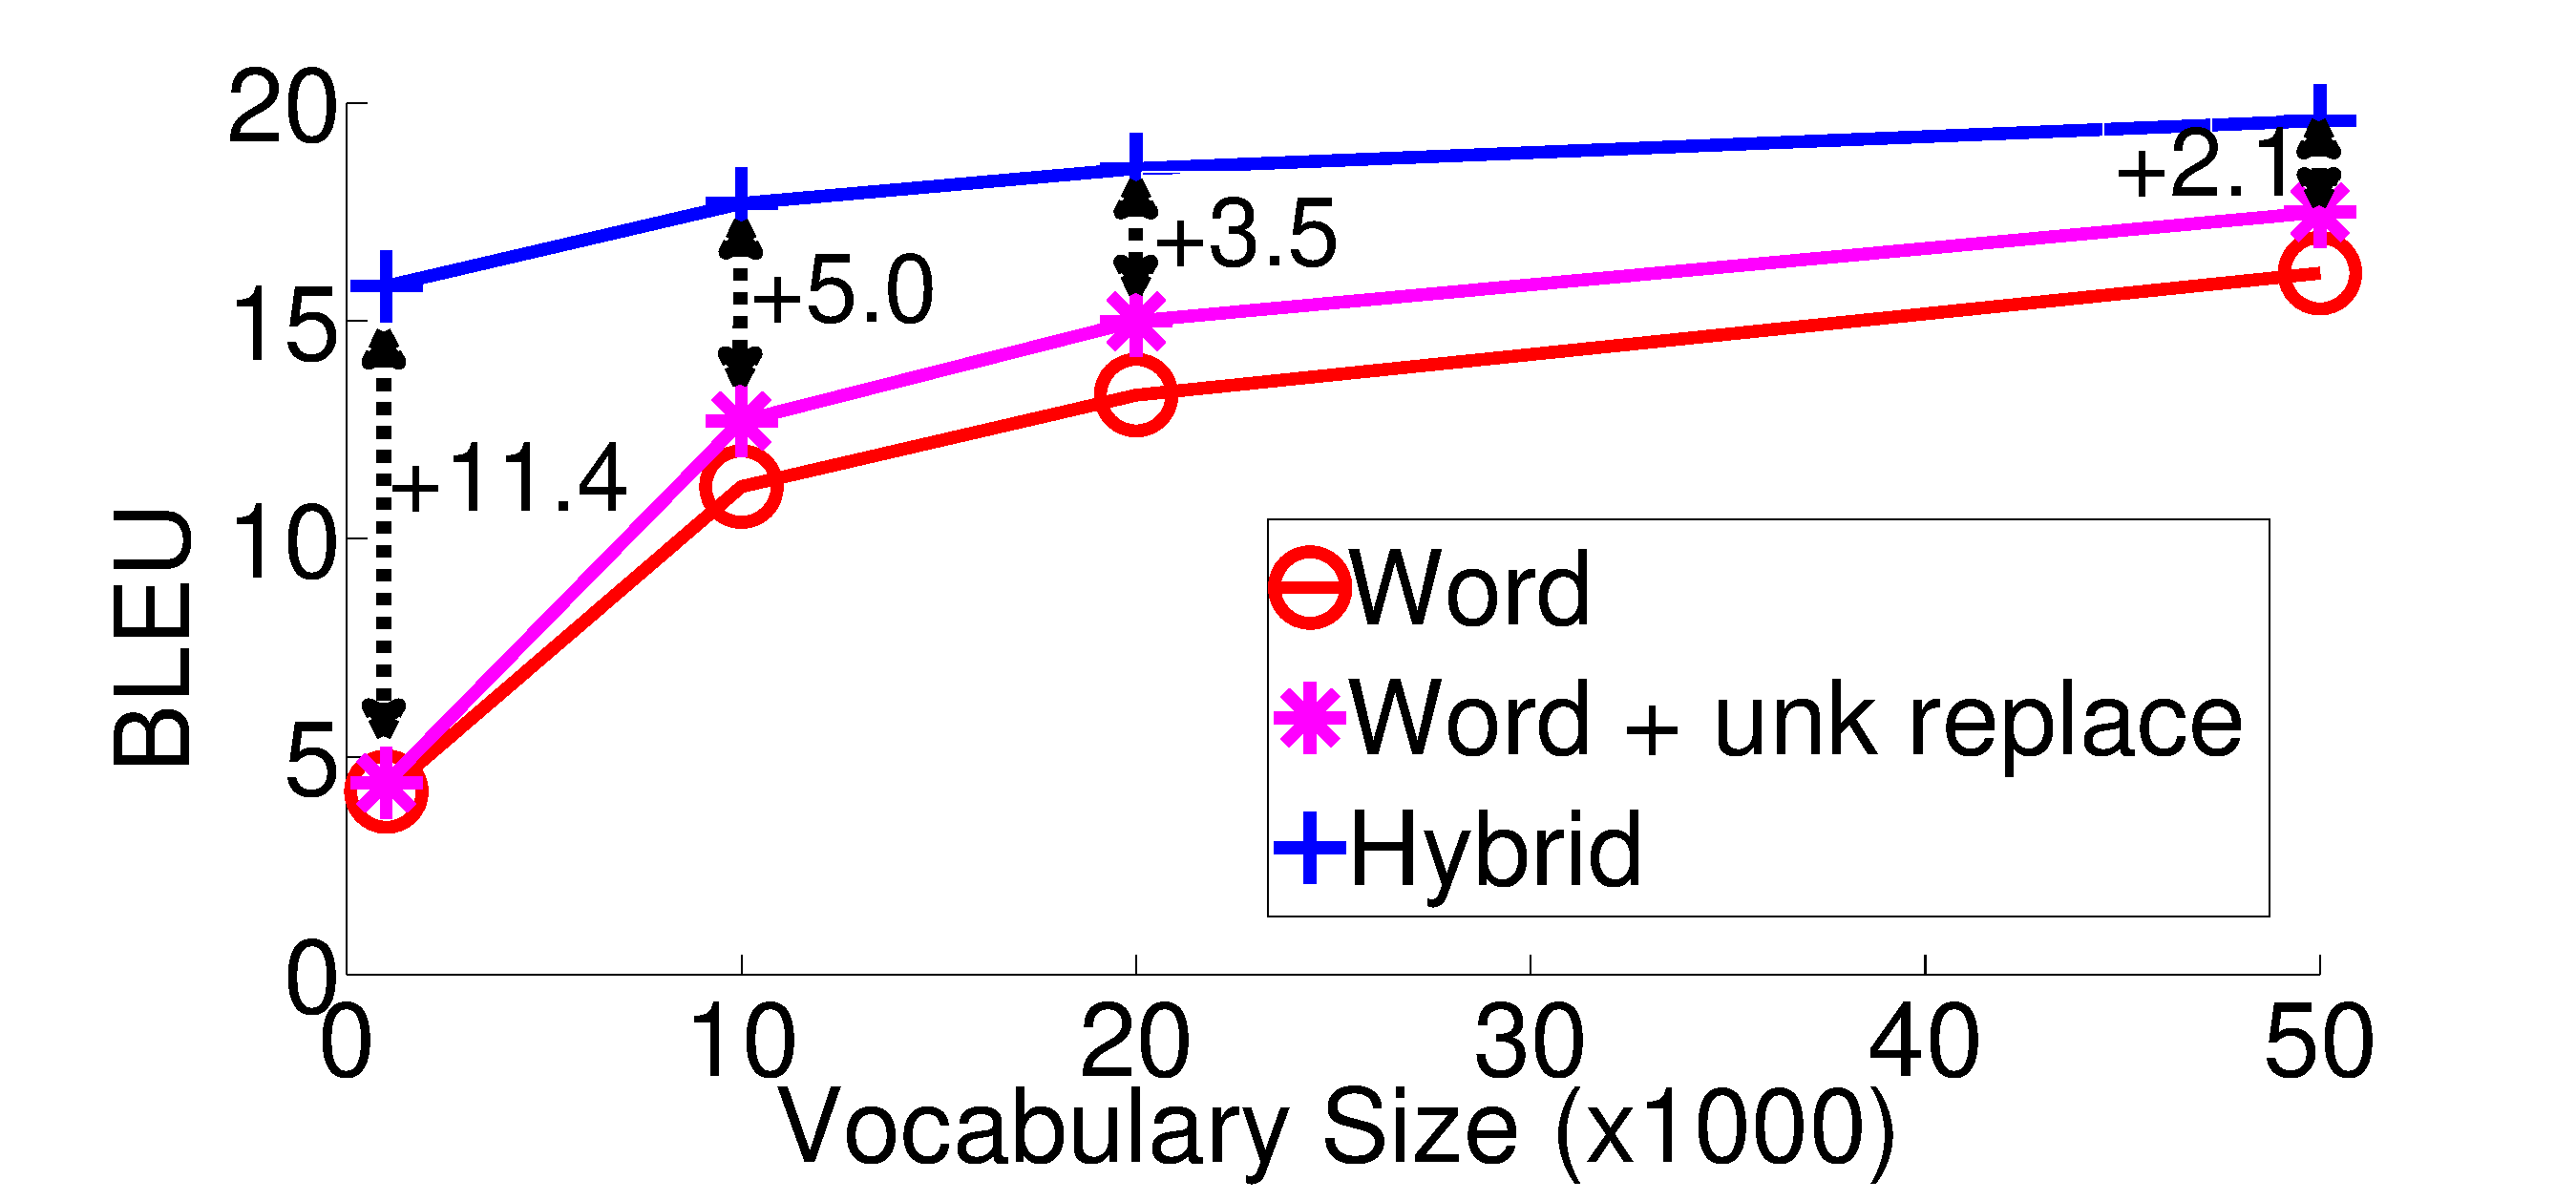
\includegraphics[width=0.7\textwidth, clip=true, trim= 0 0 0 0]{img/5-vocab}
\caption[Vocabulary size effect]{{\bf Vocabulary size effect} -- shown are the performances of different
systems as we vary their vocabulary sizes. We highlight the improvements obtained
by our hybrid models over word-based systems which already handle unknown words.}
\label{f:vocab}
\end{figure}


\begin{figure*}%[tbh]
\centering
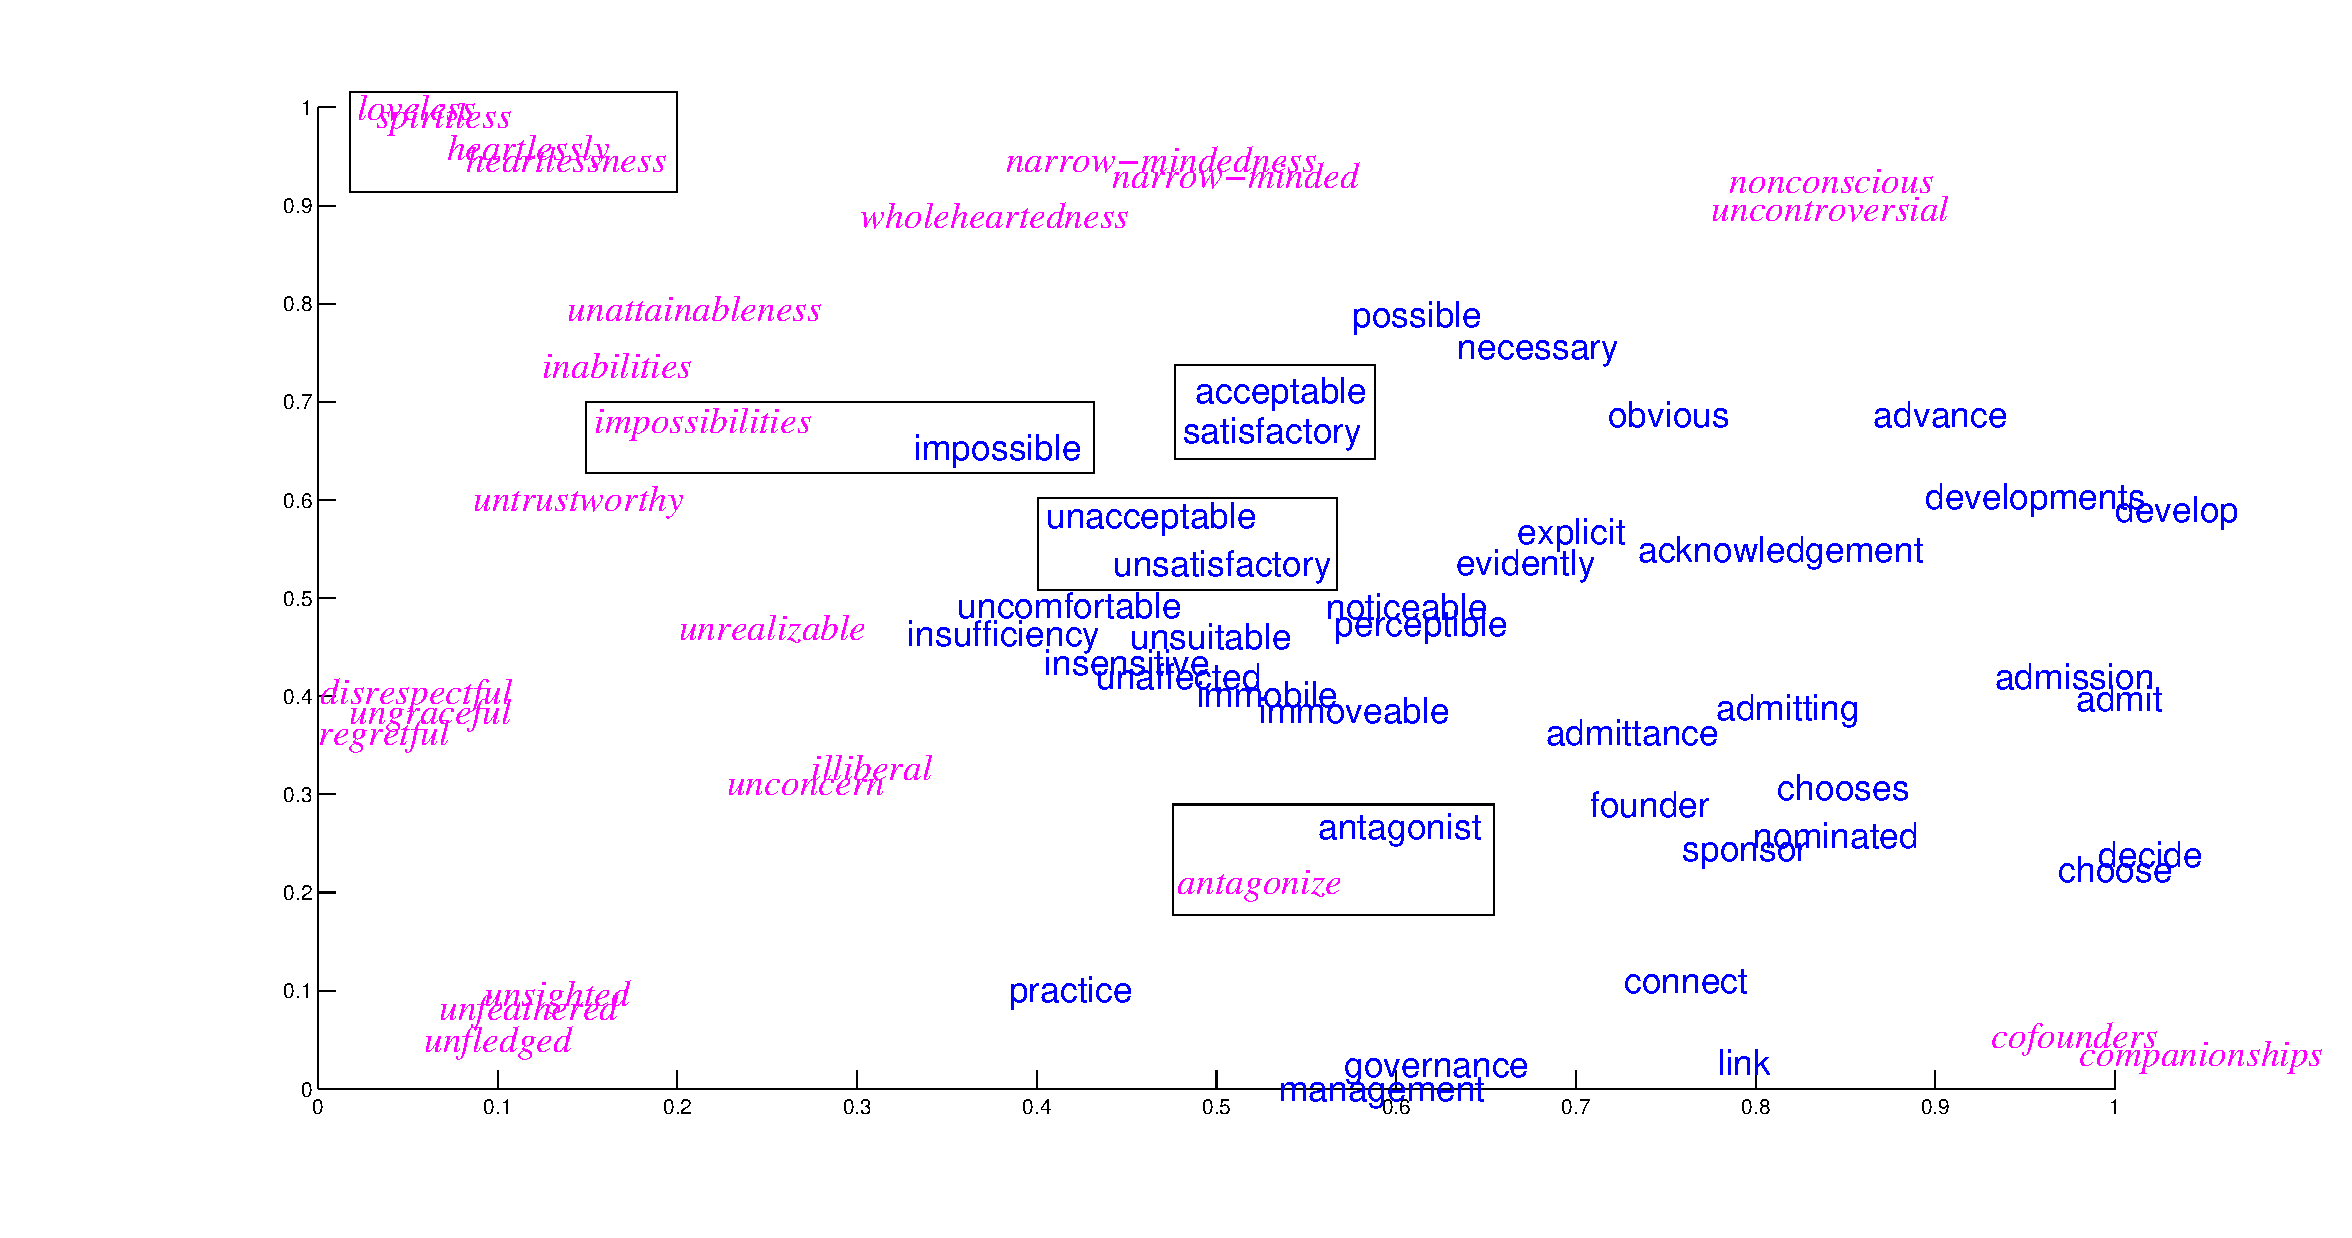
\includegraphics[width=\textwidth, clip=true, trim= 100 50 0 20]{img/5-emb}
\caption[Barnes-Hut-SNE visualization of source word representations]{{\bf Barnes-Hut-SNE visualization of source word representations} --
shown are sample words from the {\it Rare Word} dataset. We differentiate two types of
embeddings: {\color{blue} frequent} words in which encoder embeddings are looked up directly and {\it {\color{magenta} rare}} words
where we build representations from characters. Boxes highlight examples that
we will discuss in the text. We use the hybrid model \model{} in this visualization.}
\label{f:visual}
\end{figure*}


\section{Analysis}
\label{sec:analysis}
This section first studies the effects of vocabulary sizes towards
translation quality. We then analyze more carefully 
our character-level components by visualizing and evaluating rare word
embeddings as well as examining sample translations.

\subsection{Effects of Vocabulary Sizes}
As shown in Figure~\ref{f:vocab}, our hybrid models offer large gains of
+\gain{} BLEU points over strong word-based systems which already handle unknown words.
With only a small vocabulary, e.g., 1000 words, our hybrid approach can produce
systems that are better than word-based models that possess much larger
vocabularies. While it appears from the plot that gains diminish as we
increase the vocabulary size, we argue that our hybrid models are still
preferable since they understand word structures and can handle new complex
words at test time as illustrated in Section~\ref{subsec:samples}.
%Lastly, it is desirable to continue increasing the
%vocabulary size to see at which point we stop benefiting from the hybrid
%approach. It is also very interesting to  


\subsection{Rare Word Embeddings}
We evaluate the {\it source} character-level model by building representations
for rare words and measuring how good these embeddings are.

Quantitatively, we follow \newcite{luong13} in using the word similarity task,
specifically on the {\it Rare Word} dataset, to judge the learned representations for
complex words. The evaluation metric is the Spearman's correlation $\rho$
between similarity scores assigned by a model and by human annotators.
From the results in Table~\ref{t:word_sim}, we can see that source representations produced by
our hybrid\footnote{We look up the encoder embeddings for frequent words and build representations for
rare word from characters.}  models
are significantly better than those of the word-based one. It is noteworthy that our deep recurrent
character-level models can outperform the model of \cite{luong13}, which uses
recursive neural networks and requires a complex morphological analyzer, by a large
margin. Our performance is also competitive to the best Glove embeddings
\cite{pennington2014} which were trained on a much larger dataset.
\begin{table}[tbh!]
\centering
%\resizebox{8cm}{!}{
\begin{tabular}{c|l|c|c|c}
\multicolumn{2}{c|}{{\bf System}} & Size & $|V|$ & \bf{$\rho$}\\ %Spearman's 
  \hline
\multicolumn{2}{l|}{\cite{luong13}} & 1B & 138K & 34.4 \\
  \hdashline
\multicolumn{2}{l|}{\multirow{2}{*}{Glove \cite{pennington2014}}} & 6B & 400K & 38.1 \\
\multicolumn{2}{l|}{} & 42B & 400K & \bf{47.8} \\
  \hline
\multicolumn{4}{c}{{\it Our NMT models}}\\
  \hline
\modelword{} & Word-based & 0.3B & 50K & 20.4 \\
  \hdashline
\modelsmall{} & Hybrid & 0.3B & 10K & 42.4 \\
  \hdashline
\model{} & Hybrid & 0.3B & 50K & \bi{47.1} \\
\end{tabular}
%}
\caption[Word similarity task]{{\bf Word similarity task} -- shown are Spearman's correlation
$\rho$ on the {\it Rare Word} dataset
of various models (with different vocab sizes $|V|$). 
} 
\label{t:word_sim}
\end{table}


Qualitatively, we visualize embeddings produced by the hybrid model \model{} for
selected words in the Rare Word dataset.
Figure~\ref{f:visual} shows the two-dimensional representations of words
computed by the
Barnes-Hut-SNE algorithm \cite{bhsne}.\footnote{We run Barnes-Hut-SNE algorithm
over a set of 91 words, but filter out 27 words for displaying clarity.} It is extremely interesting to observe that
words are clustered together not only by the word structures but also by
the meanings. For example, in the top-left box,
the {\it character}-based representations for \word{loveless}, \word{spiritless}, \word{heartlessly}, and \word{heartlessness} are nearby,
but clearly separated into two groups. Similarly, in the center boxes, {\it
word}-based embeddings of
\word{acceptable}, \word{satisfactory}, \word{unacceptable}, and \word{unsatisfactory}, are
close by but separated by meanings. Lastly, the remaining boxes demonstrate that our
character-level models are able to build representations comparable to the
word-based ones, e.g., \word{impossibilities} vs.\ \word{impossible} and \word{antagonize}
vs.\ \word{antagonist}. All of this evidence strongly supports that the source
character-level models are useful and effective.

\begin{table*}%[tbh!]
\centering
\resizebox{15.5cm}{!}{
\begin{tabular}{c|c|p{15.5cm}}
%\multicolumn{2}{l}{{\bf English-German translations}}\\
%  \hline
% sent 0
%\multirow{7}{*}{1} & source & Petr \u{C}ech : \source{Transfer at} the last minute ? \\
%& human & Petr \u{C}ech : \correct{P\u{r}estup} \correct{na} posledn\'{i} chv\'{i}li ? \\
%  \cline{2-3}
%& \multirow{2}{*}{\it{word}} & Petr \u{C}ech : \unk{} na posledn\'{i} chv\'{i}li ? \\
%&  & Petr \u{C}ech : \wrong{Transfer} \correct{na} posledn\'{i} chv\'{i}li ? \\
%  \cline{2-3}
%& \it{char} & Petr \u{C}ech : \close{P\u{r}esnos} \wrong{v} posledn\'{i} chv\'{i}li ? \\
%  \cline{2-3}
%& \multirow{2}{*}{\it{hybrid}} & Petr \unk{} : \unk{} na posledn\'{i} chv\'{i}li ? \\
%&  & Petr \u{C}ech : \close{P\u{r}esnos} \correct{na} posledn\'{i} chv\'{i}li ? \\
%  \hline
%  \hline
% sent 1046 
\multirow{7}{*}{1} & source & The author \source{Stephen Jay Gould} died 20 years after
\source{diagnosis} . \\
& human & Autor \correct{Stephen Jay Gould} zem\u{r}el 20 let po
\correct{diagn\'oze} . \\
  \cline{2-3}
& \multirow{2}{*}{\it{word}} & Autor Stephen Jay \unk{} zem\u{r}el 20 let po
\unk{} . \\
&  & Autor \correct{Stephen Jay Gould} zem\u{r}el 20 let po \wrong{po} .\\
  \cline{2-3}
& \it{char} & Autor \wrong{Stepher Stepher} zem\u{r}el 20 let po
\correct{diagn\'oze} . \\
  \cline{2-3}
& \multirow{2}{*}{\it{hybrid}} & Autor \unk{} \unk{} \unk{} zem\u{r}el 20 let po
\unk{}. \\
&  & Autor \correct{Stephen Jay Gould} zem\u{r}el 20 let po \correct{diagn\'oze} .\\
  \hline
  \hline
% sent 80
\multirow{7}{*}{2} & source & As the Reverend \source{Martin Luther King
Jr.} said \source{fifty years ago} :\\
& human & Jak \correct{p\u{r}ed pades\'ati lety} \u{r}ekl reverend \correct{Martin
Luther King Jr} . : \\
  \cline{2-3}
& \multirow{2}{*}{\it{word}} & Jak \u{r}ekl reverend Martin \unk{} King \unk{}
p\u{r}ed pades\'ati lety : \\
&  & Jak \u{r}ekl reverend \correct{Martin Luther King} \wrong{\u{r}ekl}
\close{p\u{r}ed pades\'ati lety} : \\
  \cline{2-3}
& \it{char} & Jako reverend \correct{Martin Luther} \wrong{kr\'al \u{r}\'ikal}
\close{p\u{r}ed pades\'ati lety} : \\
  \cline{2-3}
& \multirow{2}{*}{\it{hybrid}} & Jak p\u{r}ed \unk{} lety \u{r}ekl \unk{} Martin
\unk{} \unk{} \unk{} : \\
&  & Jak \correct{p\u{r}ed pades\'ati lety} \u{r}ekl reverend \correct{Martin
Luther King} \close{Jr.} : \\
  \hline
  \hline
% sent 56 
%\multirow{7}{*}{2} & source &  George Webster , 28 , faced the \source{charges} during a hearing at the
%\source{High} Court in \source{Glasgow} . \\
%& human & George Webster , 28 , byl s \correct{obvin\u{e}n\'im} sezn\'amen
%b\u{e}hem sly\u{s}en\'i u \correct{Nejvy\u{s}\u{s}\'iho} soudu v \correct{Glasgow} .\\
%  \cline{2-3}
%%& \multirow{2}{*}{\it{word}} & George Webster , 28 , \u{c}elil obvin\u{e}n\'i b\u{e}hem sly\u{s}en\'i u Vrchn\'iho soudu v Glasgow . \\
%& \it{word} & George Webster , 28 , \u{c}elil \close{obvin\u{e}n\'i} b\u{e}hem
%sly\u{s}en\'i u \close{Vrchn\'iho} soudu v \correct{Glasgow} .  \\
%  \cline{2-3}
%& \it{char} & George Webster , 28 \u{c}elil \close{poplatk\r{u}m} b\u{e}hem sly\u{s}en\'i
%u \close{Vrchn\'iho} soudu v \close{Glasgowu} . \\
%  \cline{2-3}
%& \multirow{2}{*}{\it{hybrid}} & George \unk{} , 28 , \unk{} obvin\u{e}n\'i b\u{e}hem sly\u{s}en\'i u \unk{} soudu v \unk{} .\\
%&  & George Webster , 28 , \u{c}elil \close{obvin\u{e}n\'i} b\u{e}hem
%sly\u{s}en\'i u \close{Vrchn\'iho} soudu v \correct{Glasgow} . \\
%%& \multirow{2}{*}{\it{hybrid}} & George \unk{} , 28 , st\'al p\u{r}ed \unk{} p\u{r}i sly\u{s}en\'i u \unk{} soudu v \unk{} .\\
%%&  & George Webster , 28 , st\'al p\u{r}ed \correct{obvin\u{e}n\'im} p\u{r}i sly\u{s}en\'i u \close{Vrchn\'iho soudu} v \correct{Glasgow} . \\
%%&  \it{hybrid} & George Webster , 28 , \u{c}elil \close{obvin\u{e}n\'i} b\u{e}hem sly\u{s}en\'i u \correct{Nejvy\u{s}\u{s}\'iho} soudu v \correct{Glasgow} . \\
%  \hline
%  \hline
% sent 198
\multirow{7}{*}{3} & source & Her \source{11-year-old} daughter , \source{Shani Bart} , said it felt a " little bit
\source{weird} " [..] back to school . \\ %to suddenly be going 
& human & Jej\'{i} \correct{jeden\'{a}ctilet\'{a}} dcera \correct{Shani Bartov\'{a}} prozradila
, \u{z}e " je to trochu \correct{zvl\'{a}\u{s}tn\'{i}} " [..] znova do
\u{s}koly . \\ %chodit najednou
  \cline{2-3}
& \multirow{2}{*}{\it{word}} & Jej\'i \unk{} dcera \unk{} \unk{} \u{r}ekla , \u{z}e je to " trochu
divn\'e " , [..] vrac\'i do \u{s}koly .\\ %\u{z}e se najednou
&  & Jej\'i \wrong{11-year-old} dcera \correct{Shani} \wrong{,} \u{r}ekla , \u{z}e je to " trochu
\close{divn\'e} " , [..] vrac\'i do \u{s}koly . \\ %\u{z}e se najednou
  \cline{2-3}
& \it{char} & Jej\'i \correct{jeden\'actilet\'a} dcera , \correct{Shani
Bartov\'a} , \u{r}\'ikala ,
\u{z}e c\'it\'i trochu \close{divn\u{e}} , [..] vr\'atila do \u{s}koly .\\ %aby se
  \cline{2-3}
%& \multirow{2}{*}{\it{hybrid}} & Jej\'i \unk{} dcera , \unk{} \unk{} , \u{r}ekla
%, \u{z}e je to " \unk{} \unk{} " , [..] vr\'atila do \u{s}koly .\\ %aby se najednou
%&  & Jej\'i \close{jedenadvac\'at\'e} dcera , \wrong{p\u{r}\'itelkyn\u{e} Barth} , \u{r}ekla , \u{z}e je to " mali\u{c}kost 
%\close{divn\'a} " , [..] vr\'atila do \u{s}koly . \\ %aby se najednou
& \multirow{2}{*}{\it{hybrid}} & Jej\'i \unk{} dcera , \unk{} \unk{} , \u{r}ekla , \u{z}e c\'it\'i " trochu
\unk{} " , [..] vr\'atila do \u{s}koly .\\ %aby se najednou
&  & Jej\'i \correct{jeden\'actilet\'a} dcera , \wrong{Graham} \close{Bart} , \u{r}ekla , \u{z}e c\'it\'i " trochu
\close{divn\'y} " , [..] vr\'atila do \u{s}koly . \\ %aby se najednou
\end{tabular}
}
\caption[Sample translations on newstest2015]{{\bf Sample translations on newstest2015} -- %examples in both translation directions.
for each example, we show the {\it source}, {\it human} translation, and
translations of the following NMT systems: {\it word} model \modelword{},
{\it char} model \modelchar{}, and {\it hybrid} model \modelsmall{}. We show the
translations before replacing \unk{} tokens (if any) for the word-based 
and hybrid models. The following formats are used to highlight
\correct{correct}, \wrong{wrong}, and \close{close} translation segments.}
\label{t:sample}
\end{table*}


\subsection{Sample Translations}
\label{subsec:samples}

We show in Table~\ref{t:sample} sample translations between various systems. 
In the first example, our hybrid model translates perfectly. The word-based
model fails to translate \word{diagnosis} because the second \unk{} was incorrectly
aligned to the word \word{after}. The character-based model, on the other hand,
makes a mistake in translating names.

For the second example, the hybrid model surprises us when it can capture
the long-distance reordering of \word{fifty years ago} and \word{p\u{r}ed
pades\'ati lety} while the other two models do not. The word-based model
translates \word{Jr.} inaccurately due to the incorrect alignment between the
second \unk{} and the word \word{said}. The
character-based model literally translates the name \word{King} into \word{kr\'al}
which means \word{king}.

Lastly, both the character-based and hybrid models impress us by
their ability to translate compound words exactly, e.g., \word{11-year-old} and
\word{jeden\'actilet\'a}; whereas the identity copy
strategy of the word-based model fails.
%The hybrid model is better than the character-based models in many translation
%examples, e.g., ``na'', ``obvin\u{e}n\'im'', ``Glasgow'' etc. 
Of course, our hybrid model does make mistakes, e.g., it fails to translate the name
\word{Shani Bart}. 
Overall, these examples highlight how challenging translating
into Czech is and that being able to translate at the character level helps
improve the quality.

\section{Conclusion}
\label{sec:conclude}
We have proposed a novel {\it hybrid} architecture that combines the strength
of both word- and character-based models. Word-level models are fast to train
and offer high-quality translation; whereas, character-level models help achieve
the goal of open vocabulary NMT. 
We have demonstrated these two aspects through our experimental results and
translation examples.

Our best hybrid model has surpassed the performance of both the best word-based
NMT system and the best non-neural model to establish a new state-of-the-art result for 
English-Czech translation in WMT'15 with $\ensbleu{}$ BLEU.
Moreover, we have succeeded in replacing the standard unk replacement technique
in NMT with our character-level components, yielding an improvement of 
+$\gain{}$ BLEU points. Our analysis has shown that our model has the ability to
not only generate well-formed words for
Czech, a highly inflected language with an enormous and complex vocabulary, but
also build accurate representations for English source words.

Additionally, we have demonstrated the potential of purely character-based
models in producing good translations;
they have outperformed past word-level NMT models. For future work, we hope to be able to improve the memory usage and
speed of purely character-based models.




\chapter{NMT Future}
\label{c:future}

\section{Multi-task Sequence to Sequence Learning}
Multi-task learning (MTL) is an important machine learning paradigm that
aims at improving the generalization performance of a task using other related
tasks. 
Such framework has been widely studied by
\newcite{thrun96,caruana97,evgeniou04,ando05,argyriou07,kumar12}, among many
others. In the context of deep neural networks, MTL has
been applied successfully to various problems ranging from language
\cite{liu15}, to vision
\cite{donahue14},
and speech \cite{heigold13,huang2013cross}.

\begin{sloppypar}
Recently, sequence to sequence (\ssl{}) learning
\cite{kal13,sutskever14,cho14} emerges as an effective paradigm for dealing with
variable-length inputs and outputs. \ssl{} learning, at its core, uses
recurrent neural networks to map variable-length input sequences to
variable-length output sequences.  While relatively new, the \ssl{}
approach has achieved state-of-the-art results in not only its original
application -- machine translation --
\cite{luong15,jean15,luong15attn,jean15wmt,luong15iwslt}, but also image caption generation \cite{vinyals15caption},
and constituency parsing \cite{vinyals15grammar}. 
\end{sloppypar}

Despite the popularity of multi-task learning and sequence to sequence
learning, there has been little work in combining MTL with \ssl{}
learning. To the best of my knowledge, there is only one recent
publication by \newcite{dong15} which applies a \ssl{} models for machine
translation, where the goal is to translate from one language to
multiple languages.
In this work, I propose three MTL
approaches that complement one another: (a) the {\it \otm} approach -- for
tasks that can have an encoder in common, such as translation and parsing; this 
applies to the multi-target translation setting in \cite{dong15} as well, (b)
the {\it \mto} approach -- useful for multi-source
translation or tasks in which only the decoder can be easily shared,
such as translation and image captioning, and lastly, (c) the {\it \mtm} approach -- which share
multiple encoders and decoders through which I study the effect of unsupervised
learning in translation.
I show
that syntactic parsing and image caption generation improves the
translation quality between English and German by up to +$1.5$ BLEU points over
strong single-task baselines on the WMT benchmarks. 
Furthermore, I have established a new {\it state-of-the-art} result in
constituent parsing with 93.0 F$_1$.
I also explore two unsupervised learning
objectives, sequence autoencoders \cite{dai15} and skip-thought vectors
\cite{kiros15skip}, and reveal their interesting properties in the MTL setting: autoencoder helps less in terms of
  perplexities but more on BLEU scores compared to skip-thought.
%My novel findings reveal that the skip-thought objective improves
%translation while the sequence autoencoders does not.
\begin{figure}%[tbh]
\centering
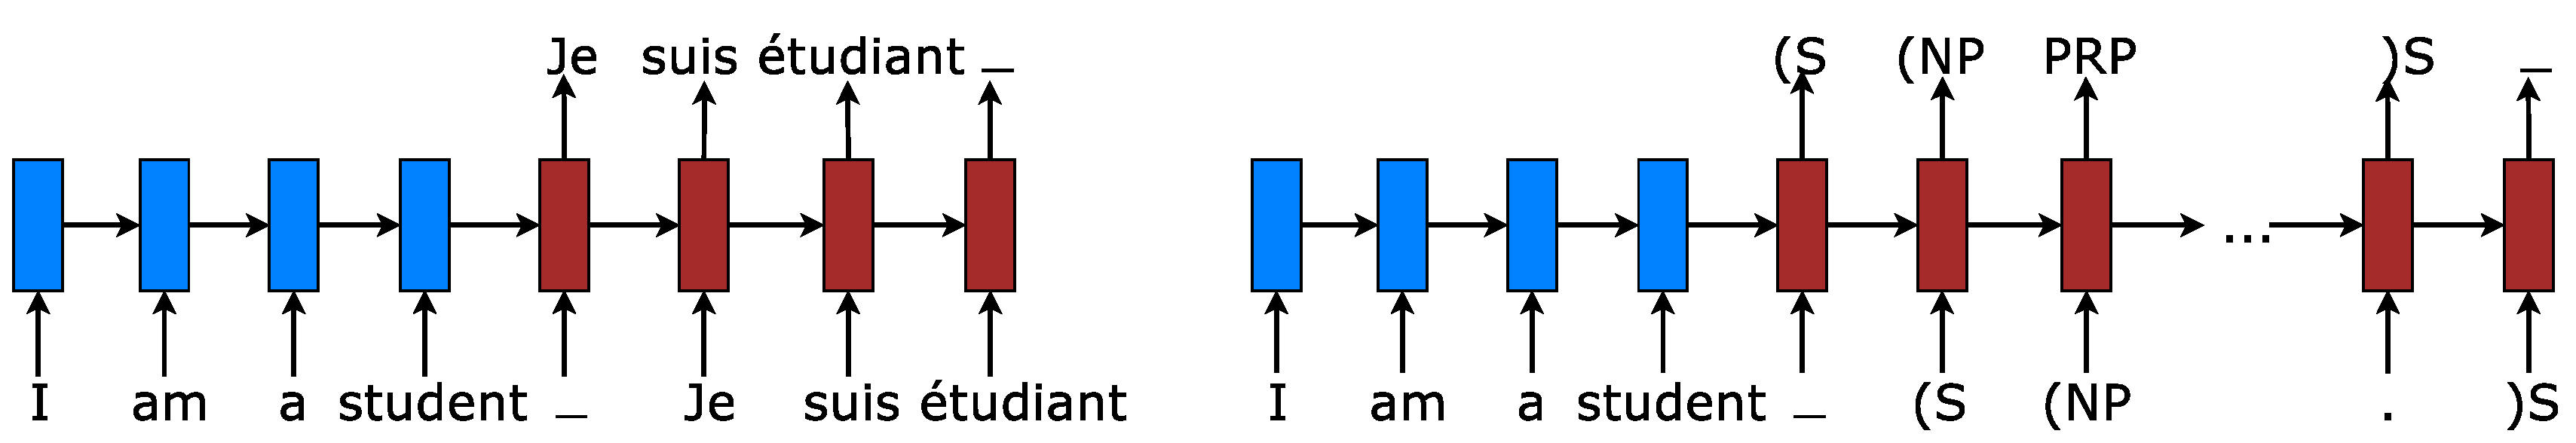
\includegraphics[width=1\textwidth, clip=true, trim= 0 0 0
0]{img/6-1_seq2seq}
\caption[Sequence to sequence learning examples]{{\bf Sequence to sequence learning examples} -- (left) machine
translation \cite{sutskever14} and ({\it right}) constituent parsing
\cite{vinyals15grammar}.}
\label{f:s2s}
\end{figure}



\begin{figure}%[tbh]
\centering
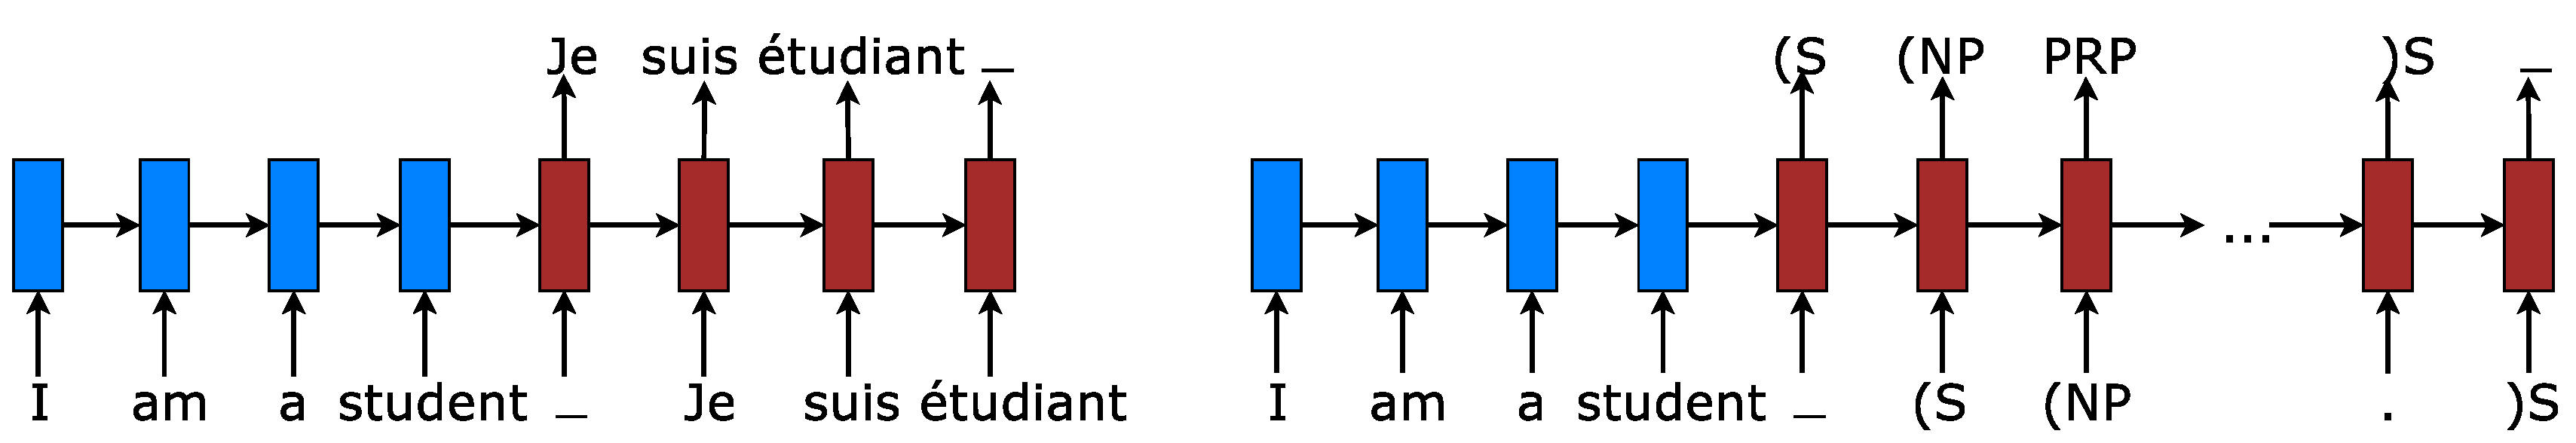
\includegraphics[width=1\textwidth, clip=true, trim= 0 0 0
0]{img/6-1_seq2seq}
\caption{{\bf Sequence to sequence learning examples} -- (left) machine
translation \citep{sutskever14} and ({\it right}) constituent parsing
\citep{vinyals15grammar}.}
\label{f:s2s}
\end{figure}


\subsection{Multi-task Sequence-to-Sequence Learning}
\label{sec:multi}
We generalize the work of \citet{dong15} to the multi-task sequence-to-sequence
learning setting that includes the tasks of machine translation (MT),
constituency parsing, and image caption generation. Depending which tasks 
involved, we propose to categorize multi-task \ssl{} learning into three general
settings.
In addition, we will discuss the unsupervised learning tasks considered as well
as the learning process.

\paragraph{One-to-Many Setting}
%\label{subsec:otm}
This scheme involves {\it one encoder} and {\it multiple decoders} for tasks in
which the encoder can be shared, as illustrated in
Figure~\ref{f:otm}. The input to each task is a sequence of
English words. A separate decoder is used to generate each sequence of
output units which can be either (a) a sequence of tags for
constituency parsing as used in \citep{vinyals15grammar}, (b) a
sequence of German words for machine translation \citep{luong15attn},
and (c) the same sequence of English words for autoencoders or a
related sequence of English words for the skip-thought objective
\citep{kiros15skip}.

\begin{figure}[tbh]
\centering
%\psgrid
%\rput(7.5,2.6){$\alpha_1=1.0$}
%\rput(7.5,1.5){$\alpha_2=0.1$}
%\rput(7.5,0.4){$\alpha_3=0.5$}
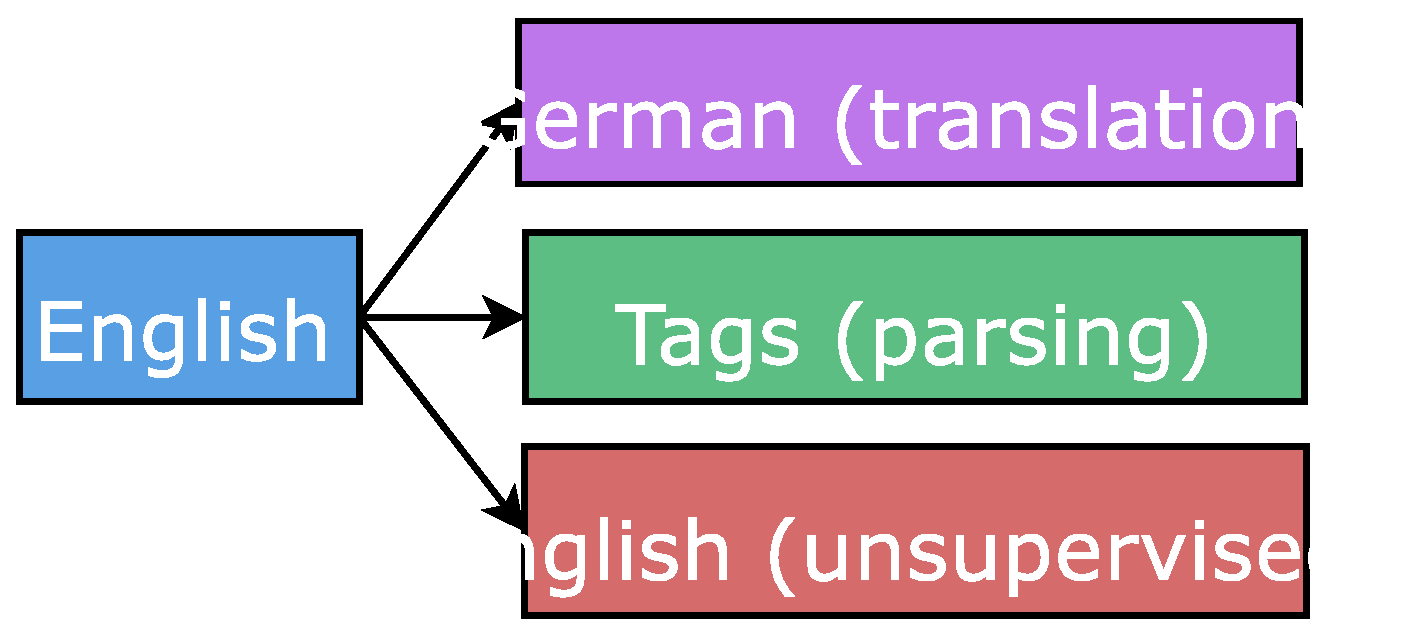
\includegraphics[width=0.45\textwidth, clip=true, trim= 0 0 0
0]{img/6-1_otm}
\caption[One-to-many Setting]{{\bf One-to-many Setting} -- one encoder, multiple decoders. This scheme
is useful for either multi-target translation as
in \cite{dong15} or between different tasks. Here, English and
German imply sequences of words in the respective languages. 
%The $\alpha$ values
%give the proportions of parameter updates that are allocated for the different tasks.
} 
\label{f:otm}
\end{figure}

\paragraph{Many-to-One Setting}
%\label{subsec:mto}
This scheme is the opposite of the {\it one-to-many}
setting. As illustrated in Figure~\ref{f:mto}, it consists of {\it multiple
encoders} and {\it one decoder}. This is useful for tasks in which only the
decoder can be shared, for example, when our tasks include machine translation
and image caption generation \citep{vinyals15caption}. In addition, from a machine
translation perspective, this setting can benefit from a large
amount of monolingual data on the target side, which is a standard
practice in machine translation system and has also been explored
for neural MT by \cite{gulcehre2015using}.

\begin{figure}[tbh]
\centering
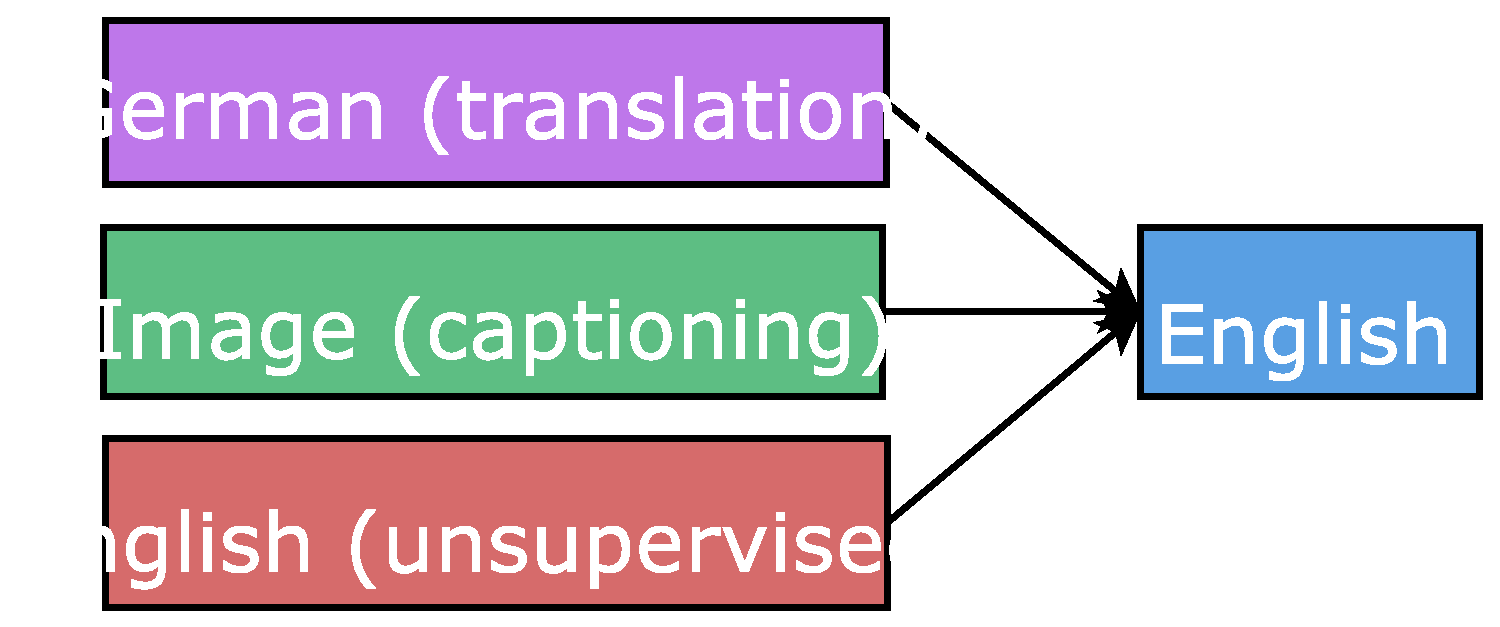
\includegraphics[width=0.5\textwidth, clip=true, trim= 0 0 0
0]{img/6-1_mto}
\caption[Many-to-one setting]{{\bf Many-to-one setting} -- multiple encoders, one decoder. This scheme
is handy for tasks in which only the decoders can be shared.}
\label{f:mto}
\end{figure}

\paragraph{Many-to-Many Setting}
%\label{subsec:mtm}
Lastly, as the name describes, this category is the most general one,
consisting of multiple encoders and multiple decoders.
%However, such
%flexibility also makes it difficult to determine which tasks should
%share which components. ---- Is it true? IS. 
%To simplify sharing, we consider a special use
%case in machine translation which involves two encoders and two
%decoders shared over three tasks.
We will explore this scheme in a translation setting that involves sharing multiple
encoders and multiple decoders.  In addition to the machine
translation task, we will include two unsupervised 
objectives over the source and target languages as illustrated in
Figure~\ref{f:mtm}.

\begin{figure}[tbh]
\centering
\includegraphics[width=0.7\textwidth, clip=true, trim= 0 0 0
0]{img/6-1_mtm}
\caption[Many-to-many setting]{{\bf Many-to-many setting} -- multiple encoders, multiple decoders. We
consider this scheme in a limited context of machine translation to utilize the large
monolingual corpora in both the source and the target languages. Here, we
consider a single translation task and two unsupervised autoencoder tasks.} 
\label{f:mtm}
\end{figure}

\paragraph{Unsupervised Learning Tasks}

Our very first unsupervised learning task involves learning {\it autoencoders} from
monolingual corpora, which has recently been applied to sequence to sequence
learning \citep{dai15}. However, in \citet{dai15}'s work, the authors
only experiment with pretraining and then finetuning, but not joint training which
can be viewed as a form of multi-task learning (MTL). As such, we are
very interested in knowing whether the same trend extends to our MTL settings.

Additionally, we investigate the use of the {\it skip-thought}
vectors \citep{kiros15skip} in the context of our MTL framework.
Skip-thought vectors are trained by training sequence to sequence
models on pairs of consecutive sentences, which makes the skip-thought
objective a natural \ssl{} learning candidate. A minor technical
difficulty with skip-thought objective is that 
the training data must consist of ordered sentences, e.g., paragraphs.  Unfortunately, in
many applications that include machine translation, we only have
sentence-level data where the sentences are unordered. To
address that, we split each sentence into two halves; we then use 
one half to predict the other half.

\paragraph{Learning}
%\label{subsec:learning}
\cite{dong15} adopted an {\it alternating} training approach, where they
optimize each task for a fixed number of parameter updates (or
mini-batches) before switching to the next task (which is a different
language pair). In our setting, our tasks are more diverse and contain
different amounts of training data. As a result, we allocate different
numbers of parameter updates for each task, which are expressed with
the {\it mixing} ratio values $\alpha_i$ (for each task $i$). Each
parameter update consists of training data from one task only. When
switching between tasks, we select randomly a new task $i$ with
probability $\frac{\alpha_i}{\sum_j \alpha_j}$.
%{\bf [Thang, make sure that it is correct]} 


Our convention is that the first task is the
{\it reference} task with $\alpha_1 = 1.0$ and the number of training
parameter updates for that task is prespecified to be $N$. A typical task $i$ will then be
trained for $\frac{\alpha_i}{\alpha_1}\cdot N$ parameter updates.
Such convention makes it easier for us to fairly compare the same reference
task in a single-task setting which has also been trained for exactly $N$
parameter updates.

When sharing an encoder or a decoder, we share both the recurrent connections
and the corresponding embeddings.

%This ensures
%fairness when comparing the performance of the reference task trained
%alone using the same number of mini-batches.
%IS:  I don't think that it follows.




\subsection{Experiments}
\label{sec:exp}
We evaluate the multi-task learning setup on a wide variety of
sequence-to-sequence tasks: constituency parsing, image caption
generation, machine translation, and a number of unsupervised learning as
summarized in Table~\ref{t:tasks}.

\paragraph{Data}
%\label{subsec:data}
Our experiments are centered around the {\it translation} task, where we aim to determine 
whether other tasks can improve translation and vice versa. We use the WMT'15 data
\citep{bojar15} for the English$\leftrightarrows$German
translation problem. Following 
\citet{luong15attn}, we use the 50K most frequent words for each
language from the training corpus.\footnote{The corpus has already been tokenized using the default
tokenizer from Moses.  Words not in these vocabularies are represented by the token
\texttt{<unk>}.} These vocabularies are then shared with other tasks, except for
parsing in which the target ``language'' has a vocabulary of 104 tags. 
We use newstest2013 (3000 sentences) as a validation set to select our
hyperparameters, e.g., mixing coefficients. For testing, to be comparable with existing results in
\citep{luong15attn}, we use the filtered
newstest2014 (2737
sentences)\footnote{\url{http://statmt.org/wmt14/test-filtered.tgz}} for the
English$\rightarrow$German translation task and newstest2015 (2169
sentences)\footnote{\url{http://statmt.org/wmt15/test.tgz}}
for the German$\rightarrow$English task.
See the summary in Table~\ref{t:tasks}.

For the {\it unsupervised} tasks, we use the English and German monolingual corpora
from WMT'15.\footnote{The training sizes reported for
the unsupervised tasks are
only 10\% of
the original WMT'15 monolingual corpora which we randomly sample from. Such reduced sizes are
for faster training time and already about three times larger than that of the parallel
data. We consider using all the monolingual data in future work.} Since in
our experiments, unsupervised tasks are always coupled with translation tasks,
we use the same validation and test sets as the accompanied translation tasks.

For {\it constituency parsing}, we experiment with two types of corpora:
\begin{enumerate}
\item a small corpus -- the widely used
Penn Tree Bank (PTB) dataset \citep{Marcus:1993:BLA} and,
\item a large corpus -- the high-confidence (HC) parse trees 
provided by \citet{vinyals15grammar}.
\end{enumerate}
The two parsing tasks, however, are evaluated on the same validation (section
22) and test (section 23)
sets from the PTB data. Note also that the parse trees have been linearized
following \citet{vinyals15grammar}. 
Lastly, for {\it image caption generation}, we use a dataset of image and caption pairs provided by
\citet{vinyals15caption}.


% together with various training details.
%\citep{vinyals15caption}\citep{luong15attn}\citep{dai15,kiros15skip}
\paragraph{Training Details}

In all experiments, following \citet{sutskever14} and \citet{luong15}, we train deep LSTM
models as follows: (a) we use 4 LSTM layers each of which has
1000-dimensional cells and embeddings,\footnote{For image caption generation, we use 1024
dimensions, which is also the size of the image embeddings.} (b) parameters are
uniformly initialized in [-0.06, 0.06], (c) we use a mini-batch size of 128, (d)
dropout is applied with probability of 0.2 over vertical connections
\citep{pham2014dropout}, (e) we use SGD with a fixed
learning rate of 0.7, (f) input sequences are reversed, and lastly, (g) we use a simple finetuning schedule -- after $x$
epochs, we halve the learning rate every $y$ epochs. The values $x$ and $y$
are referred as {\it finetune start} and {\it finetune cycle} in
Table~\ref{t:tasks} together with the number of training epochs per task.

As described in Section~\ref{subsec:multi}, for each multi-task
experiment, we need to choose one task to be the {\it reference
task} (which corresponds to $\alpha_1 = 1$). The choice of the
reference task helps specify the number of training epochs and the
finetune start/cycle values which we also when training that reference
task alone for fair comparison. To make sure our findings are
reliable, we run each experimental configuration twice and
report the average performance in the format {\it mean (stddev)}.

\begin{table}%[tbh!]
\centering
\resizebox{14cm}{!}{
\begin{tabular}{l|c|c|c|c|c|c|c|c}
\multirow{ 2}{*}{\bf{Task}} & {\bf Train} & {\bf Valid} &{\bf Test} &
\multicolumn{2}{c|}{{\bf Vocab Size}} & {\bf Train} &
\multicolumn{2}{c}{{\bf Finetune}}\\
  \cline{5-6} \cline{8-9}
  & {\bf Size}& {\bf Size}& {\bf Size} & Source & Target & {\bf Epoch} & Start & Cycle \\
  \hline
English$\rightarrow$German Translation & 4.5M & 3000 & 3003 & 50K & 50K & 12 & 8 & 1 \\
  \hline
German$\rightarrow$English Translation & 4.5M & 3000 & 2169 & 50K & 50K & 12 & 8 & 1 \\
  \hline
English unsupervised & 12.1M & \multicolumn{2}{c|}{\multirow{2}{*}{Details in
text}} & 50K & 50K & 6 & 4 & 0.5 \\
  \cline{1-2} \cline{5-9}
German unsupervised & 13.8M & \multicolumn{2}{c|}{} & 50K & 50K & 6 & 4 & 0.5 \\
  \hline
Penn Tree Bank Parsing & 40K & 1700 & 2416 & 50K & 104 & 40 & 20 & 4 \\
  \hline
High-Confidence Corpus Parsing & 11.0M & 1700 & 2416 & 50K & 104 & 6 & 4 & 0.5 \\
  \hline
Image Captioning & 596K & 4115 & -  & - & 50K & 10 & 5 & 1 \\ 
\end{tabular}
}
\caption{{\bf Data \& Training Details} -- Information about the different
datasets used in this work. For each task, we display the following
statistics: (a) the number of training examples, (b) the sizes of the
vocabulary, (c) the number of training epochs, and (d) details on when
and how frequent we halve the learning rates ({\it finetuning}).}
\label{t:tasks} 
\end{table}

\subsubsection{Results}
We explore several multi-task learning scenarios by combining a {\it
large} task (machine translation) with: (a) a {\it small} task -- Penn
Tree Bank (PTB) parsing, (b) a {\it medium-sized} task -- image
caption generation, (c) another {\it large} task -- parsing on the
high-confidence (HC) corpus, and (d) lastly, {\it unsupervised tasks},
such as autoencoders and skip-thought vectors. In terms of evaluation metrics,
we report both validation and test perplexities for all tasks. Additionally, we
also compute test BLEU scores \citep{Papineni02bleu} for the translation task.

\paragraph{Large Tasks with Small Tasks} % -- {\it translation \& parsing}}
% \label{subsubsec:big_small}
In this setting, we want to understand if a small task such as {\it
PTB parsing} can help improve the performance of a large task such as
translation.  Since the parsing task maps from a sequence of English
words to a sequence of parsing tags \citep{vinyals15grammar}, only the
encoder can be shared with an English$\rightarrow$German translation
task.  As a result, this is a {\it one-to-many}
MTL scenario ($\S$\ref{subsec:multi}).

To our surprise, the results in Table~\ref{t:big_small} suggest that
by adding a very small number of parsing mini-batches (with mixing ratio $0.01$,
i.e., one parsing mini-batch per 100 translation mini-batches), we can improve
the translation quality substantially. More concretely,
our best multi-task model yields a gain of +$1.5$ BLEU points over the
single-task baseline. It is worth pointing out that as shown in
Table~\ref{t:big_small}, our single-task baseline is very strong, even better
than the equivalent non-attention model reported in \citep{luong15attn}. Larger
mixing coefficients, however, overfit the small
PTB corpus; hence, achieve smaller gains in translation quality. 

For parsing, as \citet{vinyals15grammar} have shown that attention is crucial to
achieve good parsing performance when training on the small PTB corpus,
we do not set a high bar for our attention-free systems in this setup (better
performances are reported in Section~\ref{subsub:ll}). Nevertheless, the parsing
results in Table~\ref{t:big_small} indicate that MTL is
also beneficial for parsing, yielding an improvement of up to +$8.9$ F$_1$ points
over the baseline.\footnote{While perplexities correlate well with BLEU scores as shown
in \citep{luong15}, we observe empirically in Section~\ref{subsub:ll} that parsing perplexities are only
reliable if it is less than $1.3$. Hence, we omit parsing perplexities in
Table~\ref{t:big_small} for
clarity. The parsing test perplexities (averaged over two
runs) for the last four rows in Table~\ref{t:big_small} are 1.95, 3.05, 2.14, and 1.66. Valid perplexities
are similar.} 
It would be interesting to study how MTL can be
useful with the presence of the {\it attention} mechanism, which we
leave for future work.


\begin{table}[tbh!]
\centering
%\resizebox{14cm}{!}{
\begin{tabular}{l|c|c|c|c}
\multirow{ 2}{*}{\bf{Task}} & \multicolumn{3}{c|}{{\bf Translation}} &
\multicolumn{1}{c}{{\bf
Parsing}}\\
  \cline{2-5}
  & Valid ppl & Test ppl & Test BLEU & Test F$_1$ \\
  \hline
\citep{luong15attn} & - & 8.1 & 14.0 & -  \\
  \hline
\multicolumn{5}{c}{{\it Our single-task systems}} \\
  \hline
Translation & 8.8 (0.3) & 8.3 (0.2) & 14.3 (0.3) & -\\
  \hline
PTB Parsing & - & - & - & 43.3 (1.7) \\
  \hline
\multicolumn{5}{c}{{\it Our multi-task systems}} \\
  \hline
{\it Translation} + PTB Parsing (1x) &  8.5 (0.0) & 8.2 (0.0) & 14.7 (0.1) & 54.5 (0.4) \\
  \hline
{\it Translation} + PTB Parsing (0.1x) &  8.3 (0.1) & 7.9 (0.0) & 15.1 (0.0) &
{\bf 55.2 (0.0)}\\
  \hline
{\it Translation} + PTB Parsing (0.01x) &  {\bf 8.2} (0.2) & {\bf 7.7} (0.2) & {\bf
15.8} (0.4) & 39.8 (2.7) \\
\end{tabular}
%}
\caption{{\bf English$\rightarrow$German WMT'14 translation \& Penn Tree Bank parsing results} --
shown are perplexities (ppl), BLEU scores, and parsing F$_1$ for various systems. For muli-task
models, {\it reference} tasks are in
italic with the mixing ratio in parentheses. Our results are averaged over two
runs
in the format {\it mean (stddev)}. Best results are
highlighted in boldface.}
\label{t:big_small}
\end{table}

\paragraph{Large Tasks With Medium Tasks} % -- {\it translation \& captioning}}
We investigate whether the same pattern carries over to a medium task
such as {\it image caption generation}. Since the image caption
generation task maps images to a sequence of
English words \citep{vinyals15caption,xu15}, only the decoder can be
shared with a German$\rightarrow$English translation task. Hence, this
setting falls under the {\it many-to-one} MTL setting ($\S$\ref{subsec:multi}).

The results in Table~\ref{t:big_medium} show the same trend we observed
before, that is, by training on another task for a very small
fraction of time, the model improves its performance on its main task.
Specifically, with 5 parameter updates for image caption generation per 100
updates for translation (so the mixing ratio of $0.05$), we obtain a 
gain of +$0.7$ BLEU scores over a strong single-task baseline. Our baseline is
almost a BLEU point better than the equivalent non-attention model reported in
\cite{luong15attn}.
%When the {\it reference} task is image caption generation, MTL is still
%useful.\footnote{See
%Section~\ref{subsec:learning} on the use of reference tasks for fair
%comparison.} For every captioning parameter update, if the model also performs
%MTL with 2 translation minibatches (a mixing ratio of $2$), a gain of +$3.3$ points in
%terms of image caption generation perplexity can be achieved.

\begin{table}[tbh!]
\centering
%\resizebox{14cm}{!}{
\begin{tabular}{l|c|c|c|c}
\multirow{ 2}{*}{\bf{Task}} & \multicolumn{3}{c|}{{\bf Translation}} &
\multicolumn{1}{c}{{\bf
Captioning}}\\
  \cline{2-5}
  & Valid ppl & Test ppl & Test BLEU & Valid ppl \\ % & Test ppl \\
  \hline
\citep{luong15attn} & - & 14.3 & 16.9 & - \\ %& - \\
  \hline
\multicolumn{5}{c}{{\it Our single-task systems}} \\
  \hline
Translation & 11.0 (0.0) & 12.5 (0.2) & 17.8 (0.1) & - \\ %& - \\
  \hline
Captioning & - & - & - & 30.8 (1.3) \\ % & \\
%Captioning (2 layer) & - & 29.4 (0.3) \\
%Captioning (1 layer) & - & 28.4 (0.1) \\
  \hline
\multicolumn{5}{c}{{\it Our multi-task systems}} \\
  \hline
{\it Translation} + Captioning (1x) & 11.9 & 14.0 & 16.7 & 43.3 \\ % & 43.0 \\
{\it Translation} + Captioning (0.1x) &  10.5 (0.4) & 12.1 (0.4) & 18.0 (0.6) &
{\bf 28.4} (0.3) \\ %& {\bf 27.9} (0.2) \\
{\it Translation} + Captioning (0.05x) &  {\bf 10.3} (0.1) &  {\bf 11.8} (0.0) &
{\bf 18.5} (0.0) & 30.1 (0.3) \\ % & 29.8 (0.5)\\
{\it Translation} + Captioning (0.01x) &  10.6 (0.0) & 12.3 (0.1)& 18.1 (0.4) & 35.2 (1.4)
\\ % &  34.1 (1.4) \\
%  \hline
%{\it Captioning} + Translation (1x) & 25.6 & & & 30.2 & \\
%{\it Captioning} + Translation (2x) & 16.5 (1.2) & & & {\bf 27.5} (0.1) & \\
%{\it Captioning} + Translation (5x) & 12.0 (0.0) & & & 27.9 (0.0) & \\
\end{tabular}
%}
\caption{{\bf German$\rightarrow$English WMT'15 translation \& captioning results} -- shown are
perplexities (ppl) and BLEU scores 
for various tasks with similar format as
in Table~\ref{t:big_small}. {\it Reference} tasks are in italic with mixing
ratios in parentheses. The average results of 2 runs are in {\it
mean (stddev)} format.} %; others are for 1 run only.} 
%Note that the captioning tasks are trained and tested
%using the same English vocabulary as the translation tasks with 50K words.}
\label{t:big_medium}
\end{table}


\paragraph{Large Tasks with Large Tasks}
\label{subsub:ll}
Our first set of experiments is almost the same as the one-to-many
big-vs-small-task setting
%in Section~\ref{subsubsec:big_small} 
which combines {\it translation}, as the reference
task, with parsing. The only difference is in terms of parsing data. Instead of using the
small Penn Tree Bank corpus, we consider a large parsing resource, the
high-confidence (HC) corpus, which is provided by \citet{vinyals15grammar}.
As highlighted in Table~\ref{t:big_big_translation}, the
trend is consistent; MTL helps boost translation quality by up
to +$0.9$ BLEU points. 
%For this case, it is expected that we do not
%get better parsing results since the multi-task model has seen very
%little parsing data compared to the single-task model.

\begin{table}[tbh!]
\centering
%\resizebox{14cm}{!}{
\begin{tabular}{l|c|c|c}
\multirow{ 2}{*}{\bf{Task}} & \multicolumn{3}{c}{{\bf Translation}}\\
  \cline{2-4}
  & Valid ppl & Test ppl & Test BLEU\\
  \hline
\citep{luong15attn} & - & 8.1 & 14.0 \\
  \hline
\multicolumn{4}{c}{{\it Our systems}} \\
  \hline
Translation & 8.8 (0.3) & 8.3 (0.2) & 14.3 (0.3)\\
  \hline
{\it Translation} + HC Parsing (1x) &  8.5 (0.0) & 8.1 (0.1) & 15.0 (0.6) \\
{\it Translation} + HC Parsing (0.1x) &  {\bf 8.2} (0.3) & {\bf 7.7} (0.2) &
{\bf 15.2} (0.6)\\
{\it Translation} + HC Parsing (0.05x) &  8.4 (0.0) & 8.0 (0.1) & 14.8 (0.2) \\
\end{tabular}
%}
\caption{{\bf English$\rightarrow$German WMT'14 translation} -- shown are
perplexities (ppl) and BLEU scores of various translation models. Our
multi-task systems combine translation and parsing on the
high-confidence corpus together. Mixing
ratios are in parentheses and the average results over 2 runs are in {\it
mean (stddev)} format. Best results are bolded.}
\label{t:big_big_translation}
\end{table}

The second set of experiments shifts the attention to {\it parsing} by having it as the reference task. 
We show in Table~\ref{t:big_big_parsing} results that combine parsing with
either (a) the English autoencoder task or (b) the English$\rightarrow$German
translation task. Our models are compared against the best attention-based systems in
\citep{vinyals15grammar}, including the state-of-the-art result of 92.8 F$_1$.

\begin{table}[tbh!]
\centering
%\resizebox{14cm}{!}{
\begin{tabular}{l|c|c}
\multirow{ 2}{*}{\bf{Task}}& \multicolumn{2}{c}{{\bf
Parsing}}\\
  \cline{2-3}
  & Valid ppl & Test F$_1$\\
  \hline
  \hline
LSTM+A \citep{vinyals15grammar} &  - & 92.5 \\
LSTM+A+E \citep{vinyals15grammar} & - & {\bf 92.8} \\
  \hline
\multicolumn{3}{c}{{\it Our systems}} \\
  \hline
HC Parsing & 1.12/1.12 & 92.2 (0.1) \\
  \hline
{\it HC Parsing} + Autoencoder (1x) & 1.12/1.12 & 92.1 (0.1) \\
{\it HC Parsing} + Autoencoder (0.1x) & 1.12/1.12 & 92.1 (0.1) \\
{\it HC Parsing} + Autoencoder (0.01x) & 1.12/1.13 & 92.0 (0.1) \\
  \hline
{\it HC Parsing} + Translation (1x) & 1.12/1.13 & 91.5 (0.2) \\
{\it HC Parsing} + Translation (0.1x) & 1.13/1.13 & 92.0 (0.2) \\
{\it HC Parsing} + Translation (0.05x) & {\bf 1.11/1.12} & {\bf 92.4 (0.1)} \\
{\it HC Parsing} + Translation (0.01x) & 1.12/1.12 & 92.2 (0.0) \\
  \hline
Ensemble of 6 multi-task systems & - & {\bf 93.0} \\
\end{tabular}
%}
\caption{{\bf Large-Corpus parsing results} -- shown are
perplexities (ppl) and F$_1$ scores 
for various parsing models. Mixing ratios are in parentheses and the average
results over 2 runs are in {\it mean (stddev)} format. We show the individual perplexities for all runs
due to small differences among them. For \citet{vinyals15grammar}'s parsing results, LSTM+A
represents a single LSTM with attention, whereas LSTM+A+E indicates an ensemble
of 5 systems. Important results are bolded.}
\label{t:big_big_parsing}
\end{table}


Before discussing the multi-task results, we note a few interesting
observations. First, very small parsing perplexities, close to 1.1, can be achieved with large
training data.\footnote{Training solely on the small Penn Tree Bank
corpus can only reduce the perplexity to at most $1.6$, as evidenced by poor
parsing results in Table~\ref{t:big_small}. At the same time, these parsing
perplexities are much smaller than
what can be achieved by a translation task. This is because parsing only has
$104$ tags in the target vocabulary compared to
$50$K words in the translation case. Note that $1.0$ is the theoretical
lower bound.}  
Second, our baseline system can obtain a very competitive F$_1$ score of
92.2, rivaling \citet{vinyals15grammar}'s systems. This is rather surprising
since our models do not use any attention mechanism. A closer look into these
models reveal that there seems to be an architectural difference:
\citet{vinyals15grammar} use 3-layer LSTM with 256 cells and
512-dimensional embeddings; whereas our models use 4-layer LSTM with 1000 cells and
1000-dimensional embeddings. This further supports findings in \citep{rafal16} that
larger networks matter for sequence models.

For the multi-task results, while autoencoder does not seem to help parsing,
translation does. At the mixing ratio of 0.05, we obtain a non-negligible boost of 0.2 F$_1$ 
over the baseline and with 92.4 F$_1$, our multi-task system is on par with the best single system reported in
\citep{vinyals15grammar}. Furthermore, by ensembling 6 different multi-task
models (trained with the translation task at mixing ratios of
0.1, 0.05, and 0.01), we are able to establish a new {\it state-of-the-art} result in
English constituent parsing with {\bf 93.0} F$_1$ score.

%\begin{table}[tbh!]
%\centering
%\resizebox{14cm}{!}{
%\begin{tabular}{l|c|c|c|c|c|c}
%\multirow{ 2}{*}{\bf{Task}} & \multicolumn{3}{c|}{{\bf Translation}} &
%\multicolumn{3}{c}{{\bf
%Parsing}}\\
%  \cline{2-7}
%  & Valid ppl & Test ppl & Test BLEU & Valid ppl & Test ppl & Test F$_1$\\
%  \hline
%\citep{luong15attn} & - & 8.1 & 14.0 & - & - & - \\
%  \hline
%LSTM+A \citep{vinyals15grammar} & - & - & - & - & - & 92.5 \\
%LSTM+A+E \citep{vinyals15grammar} & - & - & - & - & - & {\bf 92.8} \\
%  \hline
%\multicolumn{6}{c}{{\it Our single-task systems}} \\
%  \hline
%Translation & 8.8 (0.3) & 8.3 (0.2) & 14.3 (0.3) & - & - & - \\
%  \hline
%HC Parsing & - & - & - & 1.12/1.12& 1.12/1.12 & 92.2 (0.1) \\
%  \hline
%\multicolumn{6}{c}{{\it Our multi-task systems}} \\
%  \hline
%{\it Translation} + HC Parsing (1x) &  8.5 (0.0) & 8.1 (0.1) & 15.0 (0.6) &
%1.13/1.13 & 1.12/1.12 & - \\
%{\it Translation} + HC Parsing (0.1x) &  {\bf 8.2} (0.3) & {\bf 7.7} (0.2) &
%{\bf 15.2} (0.6) &  1.18/1.19 & 1.17/1.18 & -  \\
%{\it Translation} + HC Parsing (0.05x) &  8.4 (0.0) & 8.0 (0.1) &
%14.8 (0.2) &  1.24/1.24 & 1.22/1.23 & - \\
%  \hline
%{\it HC Parsing} + Translation (1x) & 8.4 (0.0) & 8.0 (0.1) & - & 1.12/1.13 &
%1.12/1.12 & 91.5 (0.2) \\
%{\it HC Parsing} + Translation (0.1x) & 21.2 (0.5) & 22.6 (0.6) & - & 1.13/1.13 & 1.12/1.12 & 92.0 (0.2) \\
%{\it HC Parsing} + Translation (0.05x) & 31.4 (0.4) & 34.1 (0.5) & - & {\bf
%1.11/1.12} & {\bf 1.11/1.12} & {\bf 92.4 (0.1)} \\
%\end{tabular}
%}
%\caption{{\bf English$\rightarrow$German WMT'14 translation \& Large-Corpus parsing results} -- shown are
%perplexities (ppl) and BLEU scores 
%for various tasks with similar format as
%in Table~\ref{t:big_small}. {\it Reference} tasks are in italic with mixing
%ratios in parentheses. The average results of 2 runs are in {\it
%mean (stddev)}. For parsing, we show the individual perplexities for all runs
%due to small differences. For \citet{vinyals15grammar}'s parsing results, LSTM+A
%represents a single LSTM with attention, whereas LSTM+A+E indicates an ensemble
%of 5 systems.}
%\label{t:big_big}
%\end{table}

\paragraph{Multi-tasks and Unsupervised Learning}
Our main focus in this section is to determine whether unsupervised
learning can help improve translation. Specifically, we follow the {\it
many-to-many} approach described in Section~\ref{subsec:multi} to couple
the German$\rightarrow$English translation task with two unsupervised learning
tasks on monolingual corpora, one per language.
The results in Tables~\ref{t:unsupervised_de_en} show a similar trend as before,
a small amount of other tasks, in this case the {\it autoencoder} objective with
mixing coefficient 0.05, improves the translation quality by +$0.5$ BLEU
scores. However, as we train more on the 
autoencoder task, i.e. with larger mixing ratios, the translation performance gets worse. 

\begin{table}[tbh!]
\centering
\resizebox{14cm}{!}{
\begin{tabular}{l|c|c|c|c|c}
\multirow{ 2}{*}{\bf{Task}} & \multicolumn{3}{c|}{{\bf Translation}} &
\multicolumn{1}{c|}{{\bf
German}}& \multicolumn{1}{c}{{\bf English}}\\
  \cline{2-6}
  & Valid ppl & Test ppl & Test BLEU & Test ppl & Test ppl \\
  \hline
\citep{luong15attn} & - & 14.3 & 16.9 & - & -  \\
  \hline
\multicolumn{6}{c}{{\it Our single-task systems}} \\
  \hline
Translation & 11.0 (0.0) & 12.5 (0.2) & 17.8 (0.1) & - & - \\
  \hline
\multicolumn{6}{c}{{\it Our multi-task systems with Autoencoders}}\\
  \hline
{\it Translation} + autoencoders (1.0x) &  12.3 &  13.9 & 16.0 & {\bf 1.01} & 2.10 \\ % 1.04 & 2.75 \\
{\it Translation} + autoencoders (0.1x) & 11.4 & 12.7 & 17.7 & 1.13 & {\bf 1.44} \\ % 1.19 & 1.75 \\
{\it Translation} + autoencoders (0.05x) & {\bf 10.9} (0.1) & {\bf 12.0} (0.0) &
{\bf 18.3} (0.4) & 1.40 (0.01) & 2.38 (0.39) \\
%{\it Translation} + autoencoders (2.0x) &  10.1 &  {\bf 1.05} & {\bf 1.04} \\
  \hline
\multicolumn{6}{c}{{\it Our multi-task systems with Skip-thought Vectors}}\\
  \hline
{\it Translation} + skip-thought (1x) & {\bf 10.4} (0.1) & {\bf 10.8} (0.1) & 17.3
(0.2) & {\bf 36.9} (0.1) & {\bf 31.5} (0.4) \\ %39.0 (0.2) & 38.1 (0.1) \\
{\it Translation} + skip-thought (0.1x) &  10.7 (0.0) & 11.4 (0.2) & 17.8 (0.4)
& 52.8 (0.3) & 53.7 (0.4) \\ %  51.0 (0.2) & 64.2 (0.4)\\
{\it Translation} + skip-thought (0.01x) &  11.0 (0.1) & 12.2 (0.0) & {\bf
17.8} (0.3)
& 76.3 (0.8) & 142.4 (2.7) \\ % 69.5 (0.4) & 165.3 (3.6)\\
\end{tabular}
}
\caption{{\bf German$\rightarrow$English WMT'15 translation \& unsupervised learning results} -- shown are perplexities
for translation and unsupervised learning tasks. We experiment with both {\it
autoencoders} and {\it skip-thought vectors} for the unsupervised objectives. Numbers in {\it
mean (stddev)} format are the average results of 2 runs; others are for 1 run
only.}
%shown are perplexities
%for translation and unsupervised learning tasks. We follow the same format as in
%Table~\ref{t:unsupervised_en_de}.}
\label{t:unsupervised_de_en}
\end{table}

{\it Skip-thought} objectives, on the other hand, behave differently. If we
merely look at the perplexity metric, the results are very encouraging: with
more skip-thought data, we perform better consistently across both the
translation and the unsupervised tasks. However, when computing the BLEU scores,
the translation quality degrades as we increase the mixing coefficients. We anticipate that
this is due to the fact that the skip-thought objective changes the nature of
the translation task when using one half of a sentence to predict the other
half. It is not a problem for the autoencoder objectives, however, since one can
think of autoencoding a sentence as translating into the same language.

We believe these findings pose interesting challenges in the quest towards  better
unsupervised objectives, which should satisfy the following criteria: (a)
a desirable objective should be compatible with the supervised task in focus, e.g.,
autoencoders can be viewed as a special case of translation,
and (b) with more unsupervised data, both intrinsic and extrinsic metrics
should be improved; skip-thought objectives satisfy this criterion in terms of
the intrinsic metric but not the extrinsic one.

%results with {\it
%skip-thought} objectives which improve translation performance between
%English and German in both directions. In addition, we observe
%that better translation perplexities are achieved as we increase
%the portions of unsupervised parameter updates from 
%$0.01$ to $1$. These results show that the skip-thought objective
%is better than the autoencoder as an unsupervised objective for language tasks.

%As a side note, we observe that the source-to-source unsupervised tasks
%($3^{\text{rd}}$ column) seem to benefit this MTL setting more than the
%target-to-target unsupervised tasks ($4^{\text{th}}$ column). This might be
%explained by the asymmetric structure in the sequence to sequence learning framework
%\citep{sutskever14} that no prediction is made on the source side {\bf [To thang: I don't understand
%this last point]}.

%\begin{table}[tbh!]
%\centering
%%\resizebox{8cm}{!}{
%\begin{tabular}{l|c|c|c}
%\multirow{ 2}{*}{\bf{Task}} & \multicolumn{3}{c}{{\bf Perplexity}}\\
%  \cline{2-4}
%  & Translation & English & German \\
%  \hline
%Translation& 8.8 (0.3) & - & -\\
%  \hline
%\multicolumn{4}{c}{{\it Autoencoders}}\\
%  \hline
%{\it Translation} + autoencoders (0.1x) & 9.0 &  1.37 & 3.85 \\
%{\it Translation} + autoencoders (1.0x) &  10.0 &  1.09 & 2.78 \\
%%{\it Translation} + autoencoders (2.0x) &  10.1 &  1.05 & 1.04 \\
%  \hline
%{\it Translation} + skip-thought (0.01x) & 8.6 (0.4)  & 64.1 (1.7) & 150.9
%(1.3) \\
%{\it Translation} + skip-thought (0.1x) &  8.8 (0.3) &  46.5 (0.5) & 72.7
%(9.1)\\
%{\it Translation} + skip-thought (1x) & {\bf 8.4} (0.2)  & 35.0 (0.6) &
%43.1 (1.5)\\
%\end{tabular}
%%}
%\caption{{\bf English$\rightarrow$German translation \& unsupervised learning results} -- shown are perplexities
%for translation and unsupervised learning tasks. We experiment with both {\it
%autoencoders} and {\it skip-thought vectors} for the unsupervised objectives. Numbers in {\it
%mean (stddev)} format are the average results of 2 runs; others are for 1 run
%only.}
%\label{t:unsupervised_en_de}
%\end{table}




\subsection{Conclusion}
\label{sec:conclude}

In this section, I showed that multi-task learning (MTL) can improve the
performance of the attention-free sequence to sequence model of
\citep{sutskever14}.  I found it surprising that training on syntactic
parsing and image caption data improved our translation performance, given
that these 
datasets are orders of magnitude smaller than typical translation
datasets. 
Furthermore, I have established a new {\it state-of-the-art} result in
constituent parsing with an ensemble of multi-task models.
I also showed that the two unsupervised
learning objectives, autoencoder and skip-thought, behave differently in the MTL context
involving translation. I hope that these interesting
findings will motivate future work in utilizing unsupervised data for sequence
to sequence learning.
A criticism of this work is that the sequence to sequence models do not employ
the attention mechanism \citep{bog15}.  I leave the exploration
of MTL with attention for future work.







\section{Compression of NMT Models via Pruning}

\section{Future Outlook}



\chapter{Conclusion}
\label{c:conclude}
In this dissertation, my goal is to present to the readers all of the essence of Neural Machine Translation, through which I discuss how I have contributed to the development of NMT since its birth as a fringe research project in 2014 to its well-established status as a mainstream approach for machine translation including commercial deployments in 2016. Chapter 1 -- {\it Introduction} walks the readers through the history and fundamentals of machine translation together with drawbacks of existing approaches, leading to the development of NMT. In Chapter 2 -- {\it Background}, I provide readers with all the necessary knowledge to fully understand and build a vanilla NMT, which covers details of language model and recurrent neural network, a basic building block for NMT. Several key highlights in this chapter include (a) a complete derivation for the gradients of LSTM and its backpropagation algorithm in \secref{subsec:LSTM} and (b) the forward and backpropagation steps of multi-layer NMT models in \algo{a:nmt_forward} and \ref{a:nmt_backward}. 

Chapter 3 -- {\it Copy Mechanism} starts discussing my contribution. When I was developing the work for this chapter in 2014,
%as an intern at Google Brain, 
NMT had just started with the seminal work of \newcite{sutskever14}. Despite its potential, NMT models at that time had not been able to surpass phrase-based models and suffered from the limited-vocabulary problem. Specifically, NMT models often use a single \unk{} token to represent all other words not in its vocabulary, but do not know how to handle them at translation time. My proposed copy mechanisms provide simple yet effective ways for alleviating that problem. By learning to align the target \unk{} with words on the source through additional annotations to the training data (no need to modify the models, i.e., we can treat any NMT models as a black box), we can post-process target unknown translations much easier through word dictionary translation and identity copy of source words. This approach provides a further lift to the performance of the vanilla NMT model, allowing us for the first time to build an English-French NMT system that achieves state-of-the-art performance. Looking back, one can think of how we track target unknown words as a special case of the attention mechanism.
%, which has now been the de-facto standard in NMT. 
Still, the idea of copy mechanism remains to be useful until now, especially when adapting seq2seq models to new tasks such as text summarization \cite{gu16,gulcehre16} and semantic parsing \cite{jia16}.

Chapter 4 -- {\it Attention Mechanism} includes my deep exploration of what is now the de factor standard in NMT, the attention mechanism, which improves translation quality for long sentences. At the time of my work, there has been little study in useful architectures for attention-based NMT apart from the introduction of the attention mechanism to NMT in the seminal paper of \newcite{bog15}. My work experiments with various variants of the attention mechanism and analyze the effect of different attentional components. One of the key highlights of my work is the introduction of a simple bilinear attentional function to compare source and target states which has now been widely adopted by many people, such as Harvard NLP\footnote{\url{https://github.com/harvardnlp/seq2seq-attn}}, and across different domains such as reading comprehension \cite{chen16} and dependency parsing \cite{dozat16}. I have also introduced a local attention mechanism that only focuses on a different subset of the source sentence at each time step. While I have demonstrated the effectiveness of the local attention mechanism on translation, I wish that I could have tested it over tasks that involve very long sequences which local attention was designed for. Overall, the result of this work is a new state-of-the-art NMT system for English-German, a harder language pair than English-French, which further convinces people on the superiority of NMT.

Chapter 5 -- {\it Hybrid Models} can be viewed as my continuing effort to completely solve the rare word problem in NMT which was introduced in Chapter 3.
Instead of having separate components to perform data annotation, train NMT models, and post-process, we build a single model that handles unlimited vocabulary. Motivating by the proven word-level seq2seq architecture for NMT and the flexibility of character-based models in handling complex and unknown words, we propose hybrid models translate mostly at the word level and consult the character components for rare words only. The twofold advantage of such a hybrid approach is that it is much faster and easier to train than character-based ones; at the same time, it never produces unknown words as in the case of word-based models. This advance leads us to conquer (with state-of-the-art performance) another challenging language pair, English-Czech, in which the target is a highly-inflected language with a complex vocabulary. I have also demonstrated an impressive gain from 2.1 to 11.4 BLEU points over models that already handle unknown words. Recently, there is a new trend of translating at purely subword level \cite{sennrich16sub,gnmt16} in which a segmentation algorithm is run over the data and a black-box NMT model is used in a similar spirit to the copy mechanism. While that new trend works very well for NMT, I think that the hybrid models that I propose will remain useful for new applications where segmentation of units, such as predicates in semantic parsing, is not desirable or when we want to incorporate more complex structures such as semantic representations (instead of sequences of characters) for unknown entities to existing systems.

Chapter 6 -- {\it NMT Future} examines two questions that I think are important to the future of NMT: whether other tasks can be utilized to improve translation and whether NMT models can be compressed. The former question is important because of the fact that the first NMT systems only utilize parallel corpora despite an abundant amount of available data from monolingual and multi-lingual corpora as well as data from related tasks. To answer, 
I demonstrate that translation quality can be improved with data from parsing, image caption, and unsupervised learning. My work motivates subsequent papers in building multi-lingual NMT models \cite{zoph16,firat16,gnmt16multi,ha16}.
 The latter question arises from the indispensable role of mobile devices in society nowadays and the fact that state-of-the-art NMT models are beyond the storage capacity of existing mobile gadgets. With simple pruning schemes, my results show that the parameters of NMT models can be pruned up to 80\% without any loss in performance as long as pruned models are retrained. Subsequent work \cite{kim16distill} combines our proposed pruning approach with knowledge distillation to obtain further gain in model compression. Beside the aforementioned questions, in \secref{sec:outlook}, I cover in-depth the existing research landscape, highlight potential research directions, and speculate on future elements needed to further advance NMT 

Lastly, I am fortunate to have gone through a exciting journey in developing Neural Machine Translation since its early days. I hope that this dissertation will provide useful background and inspiration for future research in building much more advanced NMT models, through which I expect the babelfish to become a reality very soon!



% -- Appendix --
\appendix
\chapter{Miscellaneous}
\label{c:misc}
\begin{lemma}
\label{l:diag_mul}
Let $\bm{u}$, $\bm{v}$ be any vectors and $\edot$ be element-wise vector multiplication, we have:
\begin{align}
\diag (\bm{u}) \cdot \bm{v} = \bm{u} \edot \bm{v}
\end{align}
\end{lemma}

\begin{lemma}
\label{l:chain_rule}
Let $l$ be a loss value that  in which we
already knew how to compute its gradient $\der{v}$ with respect to a vector $\bm{v}$. Given that
$\bm{v} = f(\bm{Wh})$, the gradients $\der{h}, \der{W}$ of the loss $l$ with respect to the vector
$\bm{h}$ and the matrix $\bm{W}$ can be derived as follows:
\begin{align}
\der{h} = \tp{\bm{W}} \cdot \paren{f'(\bm{Wh}) \edot \der{v}}
\\
\der{W} = \paren{f'(\bm{Wh}) \edot \der{v}} \cdot \tp{\bm{h}} 
\end{align}
\end{lemma}

\begin{proof}
Let $\bm{z} = \bm{Wh}$, we have the following derivations: %applying chain rules in vector calculus, 
\begin{align*}
\der{h} &= \fracder{\bm{z}}{\bm{h}} \cdot \fracder{\bm{v}}{\bm{z}}
\cdot \der{v} && \text{[Vector calculus chain rules]}\\
&= \fracder{\bm{Wh}}{\bm{h}} \cdot \fracder{f(\bm{z})}{\bm{z}}
\cdot \der{v} \\
&=\tp{\bm{W}} \cdot \diag \paren{f'(\bm{z})} \cdot \der{v} \\
&=\tp{\bm{W}} \cdot \paren{f'(\bm{Wh}) \edot \der{v}} &&
\text{[\lemmaref{l:diag_mul}]}
\end{align*}

Let $\tp{\bm{w}_i}$ be the i$^{\text{th}}$ row vector of matrix $\bm{W}$ and
$v_i, z_i$ be the i$^{\text{th}}$ elements of vectors $\bm{v}, \bm{z}$. Also
denoting $\der{w}_i, dv_i$ to be the gradients of $l$ with respect to $\bm{w}_i,
v_i$, we have:
\begin{align*}
d\bm{w}_i &= \fracder{z_i}{\bm{w}_i} \cdot \fracder{v_i}{z_i}
\cdot dv_i && \text{[Vector calculus chain rules]}\\
&= \fracder{\tp{\bm{w}_i}\bm{h}}{\bm{w}_i} \cdot f'(z_i) \cdot dv_i \\
&= \bm{h} \cdot f'(z_i) \cdot dv_i \\ 
d\tp{\bm{w}_i} &= \paren{f'(z_i) \cdot dv_i} \cdot
\tp{\bm{h}} && \text{[Tranposing]} \\
\der{W} &= \paren{f'(\bm{Wh}) \edot \der{v}} \cdot \tp{\bm{h}}
&& \text{[Concatenating row derivatives]}
\end{align*}
\end{proof}

\begin{corollary}
\label{c:chain_rule}
As a special case of \lemmaref{l:chain_rule}, when $f$ is an identity function,
i.e., $\bm{v} = \bm{Wh}$, we have:
\begin{align}
\der{h} = \tp{\bm{W}} \cdot \der{v}
\\
\der{W} = \der{v} \cdot \tp{\bm{h}} 
\end{align}
\end{corollary}

\begin{lemma}
\label{l:edot_der}
Let $\bm{u}$, $\bm{v}, \bm{s}$ be any vectors such that  $\bm{s} = \bm{u} \edot
f(\bm{v})$. Also, let $d\bm{u}$, $d\bm{v}, d\bm{s}$ be the gradients of a loss $l$ with
respect to the corresponding vectors. We have:
\begin{align}
d\bm{u} = f(\bm{v}) \edot d\bm{s} \\
d\bm{v} = f'(\bm{v}) \edot \bm{u} \edot d\bm{s} 
%d\bm{u} = \diag \paren{f(\bm{v})} \cdot d\bm{s} \\
%d\bm{v} = \diag \paren{f'(\bm{v}} \edot \bm{u}} \cdot d\bm{s} 
\end{align}
\end{lemma}

%\begin{proof}
%\begin{align}
%d\bm{u} &= \parder{\diag \paren{f(\bm{v})} \cdot d\bm{s} \\
%\end{align}
%\end{proof}

\begin{corollary}
\label{c:edot_der}
As a special case of \lemmaref{l:edot_der} when $f$ is an identity function,
i.e.,  $\bm{s} = \bm{u} \edot \bm{v}$. We have:
\begin{align}
%d\bm{u} = \diag (\bm{v}) \cdot d\bm{s} \\
%d\bm{v} = \diag (\bm{u}) \cdot d\bm{s} 
d\bm{u} = \bm{v} \edot d\bm{s} \\
d\bm{v} = \bm{u} \edot d\bm{s} 
\end{align}
\end{corollary}


%\chapter{LSTM Backpropagation}
%\subsection{Definitions}
In this section we define some additional notation that will help us to derive the necessary back-propagation equations.

\begin{definition}
Let $U$ and $V$ refer to the $n \times n$ weight matrices corresponding to the following portions of $\MB{T}_{4n \times 2n}$:
\begin{equation}
\MB{T}_{4n \times 2n} = 
\begin{bmatrix}
U_i & V_i \\
U_f  & V_f\\
U_o & V_o\\
U_{\hat{h}} & V_{\hat{h}} \\
\end{bmatrix}
\end{equation}
In particular, we will use the superscript $l$ to denote these matrices used to calculate layer $l$ in Equation (\ref{eqn:LSTMdef1}).
\end{definition}

\begin{definition}
\label{def:z}
For all $l \in \{1,\dots,L\}$ and $t \in \{1,\dots,T\}$, define the \emph{weighted inputs}
\begin{alignat*}{2}
&\zilt = U_i \MB{h_t^{l-1}} + V_i \MB{h_{t-1}^l} \hspace{50pt}
&\zflt = U_f \MB{h_t^{l-1}} + V_f \MB{h_{t-1}^l}\\
&\zolt = U_o \MB{h_t^{l-1}} + V_o \MB{h_{t-1}^l} 
&\zglt = U_{\hat{h}} \MB{h_t^{l-1}} + V_{\hat{h}} \MB{h_{t-1}^l}
\end{alignat*}
so that 
\begin{equation}
\begin{pmatrix}
\ilt \\
\flt \\
\olt \\
\glt
\end{pmatrix}
=
\begin{pmatrix}
\sigm \\
\sigm \\
\sigm \\
\tanh
\end{pmatrix}
\begin{pmatrix}
\zilt \\
\zflt \\
\zolt \\
\zglt
\end{pmatrix}
\end{equation}
where $\sigm$ and $\tanh$ are applied element-wise.
We call $\zilt$ the \emph{weighted input} to the input gate $\ilt$.
\end{definition}

\begin{definition}
Define the \emph{error} of the input, forget, output and input modulation gates at layer $l$ and time $t$ to be
\begin{alignat*}{2}
\dilt &= \fracder{L}{\zilt} \hspace{50pt}
\dflt &&= \fracder{L}{\zflt} \\
\dolt &= \fracder{L}{\zolt} \hspace{50pt}
\dglt &&= \fracder{L}{\zglt} 
\end{alignat*}
where $L$ is the loss function. Note: $\dilt$ is the partial derivative of $L$ with respect to the weighted input $\zilt$, \emph{not} $\ilt$.
\end{definition}

\begin{definition}
Define the \emph{error} of the hidden state and cell and layer $l$ and time $t$ to be
\begin{align}
\dhlt = \fracder{L}{\hlt} \hspace{50pt} \dclt = \fracder{L}{\clt}
\end{align}
where $L$ is the loss function.
\end{definition}

\subsection{Derivations}
In this section we will derive expressions for $\dhlt$, $\dclt$, $\dilt$, $\dflt$, $\dolt$, and $\dglt$ in terms of the $\MB{\delta}$ values for the $(l+1,t)$ and $(l,t+1)$ blocks. 
These expressions will enable us to do back-propagation through time and layers.
If you are not interested in the derivations, skip ahead to Section \ref{subsec:summary} to see the final back-propagation equations.
\begin{lemma}
For $l \in \{1,\dots, L-1\}$ and $t \in \{1, \dots, T-1\}$,
\begin{equation}
\dhlt = 
\begin{bmatrix}
U_i^\top & U_f^\top & U_o^\top & U_{\hat{h}}^\top & V_i^\top & V_f^\top & V_o^\top & V_{\hat{h}}^\top 
\end{bmatrix}
\begin{bmatrix}
\MB{\delta_i^l(t+1)} \\
\MB{\delta_f^l(t+1)} \\
\MB{\delta_o^l(t+1)} \\
\MB{\delta_{\hat{h}}^l(t+1)} \\
\MB{\delta_i^{l+1}(t)} \\
\MB{\delta_f^{l+1}(t)} \\
\MB{\delta_o^{l+1}(t)} \\
\MB{\delta_{\hat{h}}^{l+1}(t)} 
\end{bmatrix}
\end{equation}
where each of the $U$ and $V$ matrices are with respect to layer $l$.
\end{lemma}
Note the left matrix in the multiplication has dimensions $n \times 8n$, the right matrix $8n \times n$, and $\dhlt$ is $n \times 1$.
\begin{proof}
We prove this element-wise. For any $j=1,\dots n$:
\begin{align}
\dhlt_j = \fracder{L}{(\hlt)_j}  & \tag{definition of $\dhlt$} 
\end{align}
Now, because $\hlt$ affects $(z_i,z_f,z_o,z_{\hat{h}})$ for $(l,t+1)$ and $(l+1,t)$, we take the chain rule over these eight variables. Therefore the above equation can be written as
\begin{alignat*}{2}
\sumkn  \Bigg( \quad 
& \fracder{L}{z_i^l(t+1)_k} \fracder{z_i^l(t+1)_k}{(\hlt)_j}    
\quad 
&& + \quad \fracder{L}{z_f^l(t+1)_k} \fracder{z_f^l(t+1)_k}{(\hlt)_j}
\\
+ \quad &  \fracder{L}{z_o^l(t+1)_k} \fracder{z_o^l(t+1)_k}{(\hlt)_j} 
\quad 
&& + \quad \fracder{L}{z_{\hat{h}}^l(t+1)_k} \fracder{z_{\hat{h}}^l(t+1)_k}{(\hlt)_j}
\\
+ \quad  & \fracder{L}{z_i^{l+1}(t)_k} \fracder{z_i^{l+1}(t)_k}{(\hlt)_j} 
\quad 
&& + \quad \fracder{L}{z_f^{l+1}(t)_k} \fracder{z_f^{l+1}(t)_k}{(\hlt)_j} 
\\
+ \quad & \fracder{L}{z_o^{l+1}(t)_k} \fracder{z_o^{l+1}(t)_k}{(\hlt)_j} 
\quad
&& + \quad \fracder{L}{z_{\hat{h}}^{l+1}(t)_k} \fracder{z_{\hat{h}}^{l+1}(t)_k}{(\hlt)_j} 
\quad  \Bigg)
\end{alignat*}
First note that the first of each pair is some $\MB{\delta}$ e.g.
\begin{align}
\fracder{L}{z_i^l(t+1)_k}= \MB{\delta_i^l(t+1)} \tag{by definition}
\end{align}
The second of each pair can be evaluated like so: 
\begin{align}
\fracder{z_i^l(t+1)_k}{(\hlt)_j} &= \parfrac{(\hlt)_j} \left( U_i^l \MB{h_{t+1}^l} + V_i^l \hlt \right)_k \tag{definition of $z_i^l(t+1)$} \\
&= \parfrac{(\hlt)_j} \left( \sum_{m=1}^n (V_i^l)_{km} (\hlt)_m \right) \tag{$U_i^l \MB{h_{t+1}^l} $ does not depend on $\hlt$} \\
&= (V_i^l)_{kj} \tag{expression equals 0 except when $m=j$}
\end{align}
so the first of the eight sums can be written as 
\begin{align}
\sumkn \fracder{L}{z_i^l(t+1)_k} \fracder{z_i^l(t+1)_k}{(\hlt)_j} = 
\sumkn  \MB{\delta_i^l(t+1)} (V_i^l)_{kj} =
\left[ (V_i^l)^\top \MB{\delta_i^l(t+1)} \right]_j
\end{align}
Finding similar expressions for the other seven sums, we obtain
\begin{alignat*}{4}
\dhlt \quad = \quad \quad 
&(U_i^l)^\top \delta_i^l(t+1) \quad
&&+ \quad (U_f^l)^\top \delta_f^l(t+1) \quad 
&&+ \quad (U_o^l)^\top \delta_o^l(t+1) \quad
&&+ \quad (U_{\hat{h}}^l)^\top \delta_{\hat{h}}^l(t+1) \\
+ \quad &(V_i^l)^\top \delta_i^{l+1}(t)
&&+ \quad (V_f^l)^\top \delta_f^{l+1}(t)
&&+ \quad (V_o^l)^\top \delta_o^{l+1}(t)
&&+ \quad (V_{\hat{h}}^l)^\top \delta_{\hat{h}}^{l+1}(t)
\end{alignat*}
\end{proof}

\begin{lemma}
For $l \in \{1,\dots, L\}$ and $t \in \{1, \dots, T-1\}$,
\begin{equation}
\dclt = \MB{\delta_c^l(t+1)} \circ f^l_{t+1} + \dhlt \circ \olt \circ \tanh'(\clt)
\end{equation}
\end{lemma}
\begin{proof}
We prove this element-wise. For any $j=1,\dots n$:
\begin{align}
\dclt_j &= \fracder{L}{(\clt)_j} \tag{definition of $\dclt$}\\
&= \sumkn \fracder{L}{(\MB{c_{t+1}^l})_k} \fracder{(\MB{c_{t+1}^l})_k}{(\clt)_j} + \sumkn \fracder{L}{(\hlt)_k} \fracder{(\hlt)_k}{(\clt)_j} \tag{chain rule} 
\end{align}
The second equality follows from the fact that $\clt$ affects $\hlt$ and $\MB{c_{t+1}^l}$.
For the first part of the expression, note that
\begin{align*}
 \fracder{(\MB{c_{t+1}^l})_k}{(\clt)_j}
&= \parfrac{(\clt)_j} \left( \MB{f^l_{t+1}} \circ \MB{c^l_{t}} + \MB{i^l_{t+1}}  \circ \MB{\hat{h}^l_{t+1}}  \right)_k \tag{by definition of $\MB{c_{t+1}^l}$} \\
&= 
\begin{cases} 
\MB{f^l_{t+1}}  &\mbox{if } k=j \\
0 &\mbox{ otherwise.}
\end{cases} 
\end{align*}
For the second part, note that
\begin{align*}
\fracder{(\hlt)_k}{(\clt)_j} 
&= \parfrac{(\clt)_j} \left( \olt \circ \tanh(\clt) \right)_k \tag{by definition of $\hlt$} \\
&= 
\begin{cases} 
(\olt)_j \tanh'(\clt)_j &\mbox{if } k=j \\
0 &\mbox{ otherwise.}
\end{cases} 
\end{align*}
Combining the previous three equations and using the definitions of $\MB{\delta_c^l(t+1)}$ and $\dhlt$, we obtain
\begin{align}
\dclt_j = \MB{\delta_c^l(t+1)}_j (\MB{f^l_{t+1}})_j + \dhlt_j (\olt)_j \tanh'(\clt)_j 
\end{align}
\end{proof}

\begin{lemma}
For $l \in \{1,\dots, L\}$ and $t \in \{1, \dots, T\}$,
\begin{equation}
\dilt = \dclt \circ \sigm'(\zilt) \circ \glt
\end{equation}
\end{lemma}
\begin{proof}
We prove this element-wise. For any $j=1,\dots n$:
\begin{align} 
\dilt_j &= \fracder{L}{\zilt_j} \tag{definition of $\dilt$} \\
&= \sumkn \fracder{L}{(\clt)_k} \fracder{(\clt)_k}{\zilt_j} \tag{chain rule} \\
&= \sumkn \dclt_k \parfrac{\zilt_j} \left( \flt \circ \MB{c^l_{t-1}} + \ilt \circ \glt \right)_k \tag{definition of $\dclt$ and $\clt$} \\
&= \dclt_j \parfrac{\zilt_j} \left( \ilt \circ \glt \right)_j \tag{expression equals 0 except when $k=j$} \\
&= \dclt_j  \sigm'(\zilt)_j  (\glt)_j \tag{definition of $\ilt$ in terms of $\zilt$}
\end{align}
Note that for the second equality we took the chain rule with respect to the elements of $\clt$, because $\ilt$ affects $\clt$.
\end{proof}
\begin{lemma}
For $l \in \{1,\dots, L\}$ and $t \in \{1, \dots, T\}$,
\begin{equation}
\dflt = \dclt \circ \sigm'(\zflt) \circ \MB{c_{t-1}^l}
\end{equation} 
\end{lemma}
\begin{proof}
We prove this element-wise. For any $j=1,\dots n$:
\begin{align} 
\dflt_j &= \fracder{L}{\zflt_j} \tag{definition of $\dflt$} \\
&= \sumkn \fracder{L}{(\clt)_k} \fracder{(\clt)_k}{\zflt_j} \tag{chain rule} \\
&= \sumkn \dclt_k \parfrac{\zflt_j} \left( \flt \circ \MB{c^l_{t-1}} + \ilt \circ \glt \right)_k \tag{definition of $\dclt$ and $\clt$} \\
&= \dclt_j \parfrac{\zflt_j} \left( \flt \circ \MB{c^l_{t-1}} \right)_j \tag{expression equals 0 except when $k=j$} \\
& = \dclt_j \sigm'(\zflt)_j (\MB{c_{t-1}^l})_j \tag{definition of $\flt$ in terms of $\zflt$}
\end{align}
Note that for the second equality we took the chain rule with respect to the elements of $\clt$, because $\flt$ affects $\clt$.
\end{proof}

\begin{lemma}
For $l \in \{1,\dots, L\}$ and $t \in \{1, \dots, T\}$,
\begin{equation}
\dolt = \dhlt  \circ \sigm'(\zolt) \circ \tanh(\clt)
\end{equation} 
\end{lemma}
\begin{proof}
We prove this element-wise. For any $j=1,\dots n$:
\begin{align} 
\dolt_j &= \fracder{L}{\zolt_j} \tag{definition of $\dolt$} \\
&= \sumkn \fracder{L}{(\hlt)_k} \fracder{(\hlt)_k}{\zolt_j} \tag{chain rule} \\
&= \sumkn \dhlt_k \parfrac{\zolt_j} \left( \olt \circ \tanh(\clt) \right)_k \tag{definition of $\dhlt$ and $\hlt$} \\
&= \dhlt_j \parfrac{\zolt_j} \left( \olt \circ \tanh(\clt) \right)_j \tag{expression equals 0 except when $k=j$} \\
&= \dhlt_j \sigm'(\zolt)_j \tanh(\clt)_j \tag{definition of $\olt$ in terms of $\zolt$}
\end{align}
Note that for the second equality we took the chain rule with respect to the elements of $\hlt$, because $\olt$ affects $\hlt$.
\end{proof}

\begin{lemma}
For $l \in \{1,\dots, L\}$ and $t \in \{1, \dots, T\}$,
\begin{equation}
\dglt = \dclt \circ \ilt \circ \tanh'(\zglt)
\end{equation} 
\end{lemma}
\begin{proof}
We prove this element-wise. For any $j=1,\dots n$:
\begin{align} 
\dglt_j &= \fracder{L}{\zglt_j} \tag{definition of $\dglt$} \\
&= \sumkn \fracder{L}{(\clt)_k} \fracder{(\clt)_k}{\zglt_j} \tag{chain rule} \\
&= \sumkn \dclt_k \parfrac{\zglt_j} \left( \flt \circ \MB{c^l_{t-1}} + \ilt \circ \glt \right)_k \tag{definition of $\dclt$ and $\clt$} \\
&= \dclt_j \parfrac{\zglt_j} \left(\ilt \circ \glt  \right)_j \tag{expression equals 0 except when $k=j$} \\
&= \dclt_j (\ilt)_j \tanh'(\zglt)_j \tag{definition of $\glt$ in terms of $\zglt$}
\end{align}
Note that for the second equality we took the chain rule with respect to the elements of $\clt$, because $\glt$ affects $\clt$.
\end{proof}


\begin{lemma}
\label{lem:weight_derivs}
For all $l \in \{1,\dots,L\}$,
\begin{align*}
\fracder{L}{U_i^l} &= \sum_{t=1}^T (\MB{h_t^{l-1}}) (\dilt)^\top 
&\fracder{L}{V_i^l} &= \sum_{t=1}^T (\MB{h_{t-1}^l}) (\dilt)^\top \\
\fracder{L}{U_f^l} &= \sum_{t=1}^T (\MB{h_t^{l-1}}) (\dflt)^\top 
&\fracder{L}{V_f^l} &= \sum_{t=1}^T (\MB{h_{t-1}^l}) (\dflt)^\top \\
\fracder{L}{U_o^l} &= \sum_{t=1}^T (\MB{h_t^{l-1}}) (\dolt)^\top 
&\fracder{L}{V_o^l} &= \sum_{t=1}^T (\MB{h_{t-1}^l}) (\dolt)^\top \\
\fracder{L}{U_{\hat{h}}^l} &= \sum_{t=1}^T (\MB{h_t^{l-1}}) (\dglt)^\top 
&\fracder{L}{V_{\hat{h}}^l} &= \sum_{t=1}^T (\MB{h_{t-1}^l}) (\dglt)^\top 
\end{align*}
\end{lemma}
\begin{proof}
We will prove the identities for the input gate $i$ only; the proofs for $f$, $o$ and $\hat{h}$ are identical.
First recall Definition \ref{def:z} for the weighted input:
\begin{equation*}
\zilt = U_i \MB{h_t^{l-1}} + V_i \MB{h_{t-1}^l} 
\end{equation*}
Now, for any $j,k \in \{1,\dots,n\}$, consider the effect of $(U_i^l)_{jk}$. It maps from the $k$th element of $\MB{h_t^{l-1}}$ to the $j$th element of $\zilt$, for all $t$. Therefore applying the chain rule we obtain
\begin{align}
\fracder{L}{(U_i^l)_{jk}} &= \sum_{t=1}^T \fracder{L}{\zilt_j} \fracder{\zilt_j}{(U_i^l)_{jk}} \tag{chain rule} \\
&= \sum_{t=1}^T \dilt_j (\MB{h_t^{l-1}})_k \tag{definition of $\dilt$ and $\zilt$}
\end{align}
Therefore
\begin{align}
\fracder{L}{(U_i^l)} = \sum_{t=1}^T  (\MB{h_t^{l-1}}) (\dilt)^\top
\end{align}
The expression for $\partial L / \partial V_i^l$ is derived similarly, by noting that $(V_i^l)_{jk}$ maps from the $k$th element of $\MB{h_{t-1}^l}$ to the $j$th element of $\zilt$.
\end{proof}

\begin{corollary}
For all $l \in \{1,\dots,L\}$,
\begin{align}
\begin{bmatrix}
\partial L / \partial U_i^l & \partial L / \partial V_i^l \\
\partial L / \partial U_f^l & \partial L / \partial V_f^l \\
\partial L / \partial U_o^l & \partial L / \partial V_o^l \\
\partial L / \partial U_{\hat{h}}^l & \partial L / \partial V_{\hat{h}}^l
\end{bmatrix}
= \sum_{t=1}^T 
\begin{bmatrix}
\dilt \\
\dflt \\
\dolt \\
\dglt
\end{bmatrix}
\begin{bmatrix}
\MB{h_t^{l-1}} & \MB{h_{t-1}^l}
\end{bmatrix}
\end{align}
\end{corollary}
\begin{proof}
This is simply a rearrangement of Lemma \ref{lem:weight_derivs}.
\end{proof}




\subsection{Summary}
\label{subsec:summary}
Now we have derived all the necessary equations, we have an algorithm to calculate the necessary error values for each LSTM block, and thus calculate the derivative of the loss function with respect to our various weights.

For $l \in \{1,\dots,L-1\}$ and $t \in \{1,\dots,T\}$, we calculate $\dhlt$ as follows: 
\begin{align*}
\dhlt &= 
\begin{bmatrix}
U_i^\top & U_f^\top & U_o^\top & U_{\hat{h}}^\top & V_i^\top & V_f^\top & V_o^\top & V_{\hat{h}}^\top 
\end{bmatrix}
\begin{bmatrix}
\MB{\delta_i^l(t+1)} \\
\MB{\delta_f^l(t+1)} \\
\MB{\delta_o^l(t+1)} \\
\MB{\delta_{\hat{h}}^l(t+1)} \\
\MB{\delta_i^{l+1}(t)} \\
\MB{\delta_f^{l+1}(t)} \\
\MB{\delta_o^{l+1}(t)} \\
\MB{\delta_{\hat{h}}^{l+1}(t)} 
\end{bmatrix} \\
\dclt &= \MB{\delta_c^l(t+1)} \circ f^l_{t+1} + \dhlt \circ \olt \circ \tanh'(\clt)\\
\dilt &= \dclt \circ \sigm'(\zilt) \circ \glt \\
\dolt &= \dhlt  \circ \sigm'(\zolt) \circ \tanh(\clt) \\
\dflt &= \dclt \circ \sigm'(\zflt) \circ \MB{c_{t-1}^l} \\
\dglt &= \dclt \circ \ilt \circ \tanh'(\zglt)
\end{align*}
Note: if $t=T$ then we take $\MB{\delta^l(t+1)}$ to be zero for $\MB{i}$, $\MB{f}$, $\MB{o}$, $\MB{\hat{h}}$ and $\MB{c}$. 
\todo{if $l=L$ how do we calculate $\dhlt$?}

Once we have calculated the above error values for all $l$ and $t$, we can calculate the derivative of the loss function with respect to our various weights. In particular, for $l \in \{1,\dots,L\}$:
\begin{align*}
\begin{bmatrix}
\partial L / \partial U_i^l & \partial L / \partial V_i^l \\
\partial L / \partial U_f^l & \partial L / \partial V_f^l \\
\partial L / \partial U_o^l & \partial L / \partial V_o^l \\
\partial L / \partial U_{\hat{h}}^l & \partial L / \partial V_{\hat{h}}^l
\end{bmatrix}
= \sum_{t=1}^T 
\begin{bmatrix}
\dilt \\
\dflt \\
\dolt \\
\dglt
\end{bmatrix}
\begin{bmatrix}
\MB{h_t^{l-1}} & \MB{h_{t-1}^l}
\end{bmatrix}
\end{align*}
We then use these derivatives to apply gradient descent to $U^l$ and $V^l$.




\bibliographystyle{plainnat}
\bibliography{thesis}
\end{document}
